% ring_size_paper.tex
% Numbers and Table 1: numbers.tex and table_kstar.tex, written by make_numbers.py from the data files of the
% repository.  Figures: figures/*.pdf, written by make_figures.py.  Build: ./build.sh.  Sources of every statement:
% TRACE.md.
% Only packages of a minimal TeX installation are used: no amssymb (no \mathbb, no \nmid), no amsthm, no natbib,
% no booktabs.
\documentclass[10pt,a4paper]{article}
\usepackage[T1]{fontenc}
\usepackage{lmodern}
\usepackage[margin=2.6cm]{geometry}
\usepackage{amsmath}
\usepackage{graphicx}
\usepackage{array}
\usepackage{enumitem}
\usepackage{microtype}
\usepackage{xcolor}
\usepackage{theorem}
\usepackage[colorlinks=true,linkcolor=black,citecolor=black,urlcolor=blue!50!black]{hyperref}

% theorem environments (one counter, numbered within sections)
\newtheorem{theorem}{Theorem}[section]
\newtheorem{lemma}[theorem]{Lemma}
\newtheorem{proposition}[theorem]{Proposition}
\newtheorem{corollary}[theorem]{Corollary}
{\theorembodyfont{\upshape}
\newtheorem{remark}[theorem]{Remark}
\newtheorem{definition}[theorem]{Definition}}
\newcommand{\qedmark}{\rule{1.1ex}{1.1ex}}
\newenvironment{proof}[1][Proof]{\par\smallskip\noindent\textit{#1.}\ }{\hfill\qedmark\par\smallskip}

% notation
\newcommand{\Zn}{\mathbf{Z}/n\mathbf{Z}}      % the ring of cells
\newcommand{\st}{\{0,1\}^n}                   % state space
\newcommand{\zero}{\mathbf{0}}                % all-zero state
\newcommand{\one}{\mathbf{1}}                 % all-one state
\newcommand{\eps}{\varepsilon}
\newcommand{\cpl}[1]{\overline{#1}}           % complement of a state (or of a cycle)
\newcommand{\gmin}{\gamma_{\min}}
\newcommand{\Sel}{\mathcal{S}}                % set of noise-selected cycles
\newcommand{\Gone}{G_1}                       % one-flip graph
\newcommand{\Dc}[1]{\mathcal{D}_{#1}}         % states containing the code #1
\newcommand{\kst}{k^{*}}
\newcommand{\code}[1]{\mathtt{#1}}            % a code or a word of cells, e.g. \code{101}
\newcommand{\ndiv}{\mathrel{\not|}}           % does not divide
\newcommand{\Occ}{\operatorname{Occ}}         % rule 94: centres of occurrences of 101
\newcommand{\Fz}{\operatorname{Fz}}           % rule 94: frozen set
\newcommand{\ord}{\operatorname{ord}}
% reproducible PDF (no time stamp, no random identifier)
\ifdefined\pdfinfoomitdate \pdfinfoomitdate=1 \fi
\ifdefined\pdftrailerid \pdftrailerid{} \fi
\ifdefined\pdfsuppressptexinfo \pdfsuppressptexinfo=-1 \fi
% generated by make_numbers.py from the data files of the repository; do not edit
\newcommand{\TableNmin}{4}
\newcommand{\TableNmax}{22}
\newcommand{\TableSweepNmax}{7}
\newcommand{\TableMechNmin}{8}
\newcommand{\TableCells}{95}
\newcommand{\TableCompared}{78}
\newcommand{\TableAgree}{78}
\newcommand{\TwentySixFourCycles}{1}
\newcommand{\TwentySixFourKv}{0, 1, 1, 2, 1, 1, 2, 2}
\newcommand{\KstarTwentySixAtFour}{2}
\newcommand{\KsevenTwentySixAtSixteen}{2}
\newcommand{\KstarTwentySixAtSixteen}{2}
\newcommand{\TwentySixSixteenWith}{3}
\newcommand{\TwentySixSixteenReach}{0}
\newcommand{\TwentySixSixteenCarrier}{2}
\newcommand{\TwentySixTwentyTwoChi}{6 and 10}
\newcommand{\TwentySixEvenZero}{14, 20, 22}
\newcommand{\TwentySixEvenPos}{10, 12, 18}
\newcommand{\NinetyFourFourClosed}{1}
\newcommand{\NinetyFourFourClassSize}{2}
\newcommand{\NinetyFourFourCodes}{$\code{010}$ and $\code{101}$}
\newcommand{\KstarNinetyFourAtFour}{1}
\newcommand{\NinetyFourDoubledInK}{0 of 5 at $n=10$, 7 of 9 at $n=14$, 10 of 45 at $n=20$ and 0 of 33 at $n=22$}
\newcommand{\KposThirtyFive}{9, 12, 15, 18, 21}
\newcommand{\KposFortyFive}{8}
\newcommand{\KposSeventyThree}{9}
\newcommand{\KposTwentyTwo}{8, 14, 15, 16}
\newcommand{\KposSixty}{8, 16}
\newcommand{\KposNinety}{8, 16}
\newcommand{\KstarSixtyPos}{1}
\newcommand{\KstarNinetyPos}{2}
\newcommand{\CyclesSixtyNinetyPos}{1}
\newcommand{\KzeroThirtySeven}{11, 12, 17, 18}
\newcommand{\KzeroOneTwentyTwo}{8, 12, 16, 20, 22}
\newcommand{\NumSwitching}{13}
\newcommand{\NumOtherSwitching}{8}
\newcommand{\OpenNmin}{8}
\newcommand{\OpenNmax}{22}
\newcommand{\ZRValues}{0.00048828 at $n=22$ and 0.00045776 at $n=24$}
\newcommand{\ZRBound}{0.01}
\newcommand{\ZRNmin}{13}
\newcommand{\ZRNmax}{27}


\title{Noise-selected cycles of elementary cellular automata\\ and the arithmetic of the ring size}
\author{Frank Peterlein\thanks{Independent researcher, Berlin. ORCID
\href{https://orcid.org/0009-0002-1886-1303}{0009-0002-1886-1303}. Contact: \texttt{frnkptrln} on GitHub. See the
statement on the use of AI at the end of the paper.}}
\date{November 2026}

\begin{document}
\maketitle

\begin{abstract}
\noindent
An elementary cellular automaton on a ring of $n$ cells is perturbed by independent bit flips of small probability
$\eps$. As $\eps\to0$ the stationary law concentrates on the cycles of least stochastic potential, the
noise-selected cycles. An integer $\kst\ge0$ records how far the selected cycles are from containing all eight
neighbourhood configurations; $\kst=0$ iff they contain all of them. We determine the selected cycles and $\kst$ for
four rules, for every ring size from a small bound on. For rule 154, $\kst=1$ if $n$ is a power of two and $\kst=0$
otherwise ($n\ge3$). For rules 43 and 142, $\kst=1$ if $4$ divides $n$ and $\kst=0$ otherwise ($n\ge4$). For rule 94,
$\kst=1$ if $3$ divides $n$ ($n\ge6$) and $\kst=0$ if not ($n\ge5$); the ring sizes $3$ and $4$ are not covered, and
$n=4$ is an exception to this pattern: there the computed value is $\kst=\KstarNinetyFourAtFour$ although $3$ does not
divide $4$. For rule 26 on $2^k$ cells the zero state is the only selected cycle ($k\ge2$), $\kst$ is $1$ or $2$ for
$k\ge3$, and $\kst=1$ for odd $k\ge3$; for even $k$ the value is computed for $k=2$ and $k=4$ only, and for the other
ring sizes $\kst$ is not determined by a proof. The proofs use that the
selected set is a union of closed classes of the graph of one-flip transitions between cycles, a restatement of
known results on stochastic stability, and they share one structure: a quantity that is conserved or monotone along
orbits, a description of the periodic states, and one-flip moves that change the quantity by a fixed amount.
\end{abstract}

\section{Introduction}

\paragraph{The question.}
Let $F$ be the global map of an elementary cellular automaton on a ring of $n$ cells. $F$ has finitely many cycles, in
general many. Suppose that after every step each cell is flipped independently with a small probability $\eps$. The
perturbed automaton is an ergodic Markov chain, and as $\eps\to0$ its stationary law concentrates on some of the
cycles of $F$. Which ones is decided by counting flips. The resistance of a path between two cycles is the number of
flips it needs, and the cycles that carry weight in the limit are those of least stochastic potential, a minimum
over spanning trees of sums of resistances (Section~\ref{sec:setting}). We call them \emph{noise-selected}. The
question of this paper is which cycles are noise-selected, as a function of $n$.

For the rules treated here the answer depends on the arithmetic of $n$, for two reasons. A state that is periodic
in space with period $p$ exists on the ring only if $p$ divides $n$. Under rules 43 and 142 the state
$(\code{0011})^{n/4}$, and under rule 94 the state $(\code{011})^{n/3}$, has a cycle that no single flip can leave
and that every other cycle can reach by single flips; when it exists it is selected, alone or with its rotations. And on the states whose ones lie on cells of one
parity, rules 154 and 26 act as the linear rule 90, which sends every state to the zero state exactly when $n$ is a
power of two.

We record the outcome by an integer $\kst\ge0$, defined in Section~\ref{sec:setting} from the potentials and
resistances; $\kst=0$ iff the states of the noise-selected cycles jointly contain all eight codes, that is, all
eight configurations of a cell and its two neighbours. In \cite{PeterleinNote}, $\kst$ is the order in $\eps$ of the
rate $\rho(\eps)\sim a\,\eps^{\kst}\log\frac1\eps$ at which the rule can be identified from a trajectory of the
perturbed automaton, and it was computed there for small rings. A study that accompanies that note~\cite{PeterleinStudy} computed $\kst$
for the \NumSwitching{} classes of rules for which it changes with $n$, for $n=\OpenNmin,\dots,\OpenNmax$ (data file
\texttt{data/ring\_size/mechanisms.csv} of the repository named at the end). The present paper proves the dependence
on $n$ for four of these classes, for every $n$ from the bounds stated in Theorem~\ref{thm:main} on, and part of it
for a fifth.

\paragraph{Results.}
For rule 154, $\kst=1$ if $n$ is a power of two and $\kst=0$ otherwise, for every $n\ge3$. For rules 43 and 142,
$\kst=1$ if $4\mid n$ and $\kst=0$ otherwise, for every $n\ge4$. For rule 94, $\kst=1$ for every $n\ge6$ with
$3\mid n$ and $\kst=0$ for every $n\ge5$ with $3\ndiv n$ (Theorem~\ref{thm:main}). For rule 94 the ring sizes $n=3$
and $n=4$ are not covered, and $n=4$ does not follow the pattern: the computed value is
$\kst=\KstarNinetyFourAtFour$ (Remark~\ref{94:rem:small}). In each case covered by the theorem the set of
noise-selected cycles and the eight indices $k_v$ behind $\kst$ are determined: the zero state alone, or all cycles
(rule 154); the cycle of $(\code{0011})^{n/4}$, or the cycles on the two levels of the number of walls next to $n/2$
(rules 43, 142); the three rotations of $(\code{011})^{n/3}$, or one closed class that contains every cycle with an
occurrence of $\code{101}$ (rule 94). For rule 26 on $n=2^k\ge4$ cells the zero state is the only noise-selected
cycle (Theorem~\ref{26:thm:main}); for $k\ge3$, $\kst$ is $1$ or $2$, and $\kst=1$ if $k$ is odd
(Proposition~\ref{26:prop:indices}, proved in Appendix~\ref{app:26}). For even $k$ the value is computed for $k=2$
and $k=4$ ($\kst=\KstarTwentySixAtFour$ at $n=4$ and $\kst=\KstarTwentySixAtSixteen$ at $n=16$) and open for
$k\ge6$. For even $n$ that
is not a power of two it is proved that $\Gone$ has one closed class and that $\kst=0$ iff this class contains a cycle
with the code $\code{111}$ (Proposition~\ref{26:prop:even}, proved in Appendix~\ref{app:26}); whether it does is
computed for $n\le\OpenNmax$ and open in general. Odd $n$ is not treated
(Sections~\ref{sec:26} and~\ref{sec:open}). The general tool is Theorem~\ref{thm:A}: the noise-selected set is a
union of closed classes of the one-flip graph, whose edges are the transitions between cycles that need one flip.
The proofs have a common structure, which Section~\ref{sec:mechanism} states once. Table~\ref{tab:kstar} compares
the theorems with exact computations for $n\le\TableNmax$.

\paragraph{What was known.}
Which cycles small noise selects is described by the stochastic potential of the theory of stochastic stability;
for the present model the order of every stationary probability is determined in \cite{PeterleinNote}. That the
selection can be read off the steps of cost one is known in that theory: Ellison~\cite{Ellison2000} attributes a
lemma of this kind to Samuelson~\cite{Samuelson1994} and to N\"oldeke and Samuelson~\cite{NoldekeSamuelson1993}, and
Theorem~\ref{thm:A} restates results of these authors. Bagnoli, Baia and
Matteuzzi~\cite{BagnoliBaiaMatteuzzi2025} iterate the chain of single-flip jumps between attractors for all classes
of elementary rules at one ring size. The building blocks used for the individual rules are known as well: rule 90
is nilpotent on $2^k$ cells and, for $3\mid n$, fixes the rotations of
$(\code{011})^{n/3}$~\cite{MartinOdlyzkoWolfram1984}; rule 154 is reversible on rings of odd
size~\cite{BhattacharjeeDas2019,Fedoriaka2025,NobeYura2004}; the wall map carries rules 142 and 43 onto rules 226
and 184~\cite{Boccara1993,Fuks2005,Fuks2005b}, and both conserve the number of walls~\cite{Fuks2005,Fuks2005b}.
Which cycles the noise selects as a function of $n$ was not found in the sources reached. Section~\ref{sec:related}
says what was read of each reference and lists what was not; no claim of novelty is made beyond that.

\paragraph{Status of the proofs.}
The proofs are by hand and use no computation. They were written and checked in the sessions described in the
statement at the end of the paper, and have not been through peer review. The proofs for rules 43
and 142, for rule 94 with $3\ndiv n$ and for rule 26 were each verified by a separate session. For rule 26 this
covers every statement of Section~\ref{sec:26} and of Appendix~\ref{app:26}: the verification excluded none of
them. It found one false sentence without consequence, in the source of Lemma~\ref{26:lem:domain}(c), which is
corrected, and no other error. It did not re-prove Theorem~\ref{thm:A}, which Proposition~\ref{26:prop:even} uses
and which was checked by the verification of the ring-size study. The proofs for rule 154 and for rule 94 with $3\mid n$
(Section~\ref{sec:154}, Lemma~\ref{94:lem:crystal} and part (i) of Theorem~\ref{94:thm:main}) have not been verified
by a separate session. Every computed value in the text and in
Table~\ref{tab:kstar} is taken from a data file of the repository by a script.

\section{Setting}\label{sec:setting}

\subsection{Rule, ring, noise}
Fix $n\ge 3$. The \emph{cells} are the elements of $\Zn$; indices are always taken mod $n$. A \emph{state} is a word
$x=(x_i)_{i\in\Zn}\in\st$. Sums of bits and of states are taken mod $2$. We write $\zero$ and $\one$ for the two
constant states, $e_j$ for the state with a single one at cell $j$, and call $x+e_j$ the \emph{flip of cell $j$} of $x$;
$|x|$ is the number of ones of $x$, $\cpl{x}=x+\one$ the complement, $\sigma$ the rotation, $(\sigma x)_i=x_{i-1}$, and
$\rho$ the reflection, $(\rho x)_i=x_{-i}$. An elementary rule is a map $f\colon\{0,1\}^3\to\{0,1\}$; rule number $N$ is
the map with $f(a,b,c)$ equal to the bit of weight $2^{4a+2b+c}$ in the binary expansion of $N$. The global map is
\[
(Fx)_i=f(x_{i-1},x_i,x_{i+1}),\qquad i\in\Zn ,
\]
and $F\sigma=\sigma F$. A \emph{code} is a word $v=abc\in\{0,1\}^3$, typeset $\code{101}$; a state $x$ \emph{contains}
$v$ if $(x_{i-1},x_i,x_{i+1})=v$ for some cell $i$, and $\Dc{v}$ is the set of states that contain $v$.

For $0<\eps<\tfrac12$ the noisy automaton is the Markov chain $X_{t+1}=F(X_t)+Z_t$ on $\st$, where the $Z_t$ are
independent and each has $n$ independent Bernoulli($\eps$) bits. Its kernel is
\[
P_\eps(y\mid x)=\eps^{\,r(x,y)}(1-\eps)^{\,n-r(x,y)},\qquad r(x,y)=H(Fx,y),
\]
with $H$ the Hamming distance; $r(x,y)$ is the \emph{resistance} of the step from $x$ to $y$, the number of flips that
the step needs. The kernel is positive, so the chain has a unique stationary law $\pi_\eps$, of full support. This is
the model of \cite{PeterleinNote}.

\subsection{Cycles, resistances, potentials}
A state $x$ is \emph{periodic} if $F^tx=x$ for some $t\ge1$; a \emph{cycle} is the orbit of a periodic state. The
cycles are $C_1,\dots,C_m$; throughout, $m$ is their number. The orbit of every state $x$ enters exactly one cycle; we
say that the orbit of $x$ \emph{ends on} that cycle. A \emph{path} is a finite sequence of states; its resistance is
the sum of the resistances of its steps. A step has resistance $0$ iff it is a step of $F$. For sets of states $A$, $B$
let $R(A\to B)$ be the least resistance of a path from a state of $A$ to a state of $B$, and for cycles let
\[
V(C,C')=R(C\to C').
\]
The \emph{stochastic potential} $\gamma(C)$ of a cycle $C$ is the least weight of a spanning in-tree on the set of
cycles rooted at $C$, that is, of a set of $m-1$ edges $D\to D'$ between distinct cycles, one out of every cycle
$D\ne C$, without directed circuit; the weight of an edge $D\to D'$ is $V(D,D')$, and the weight of a tree is the sum
of the weights of its edges. This is the stochastic potential of the theory of stochastic stability
(Section~\ref{sec:related}). Let $\gmin=\min_C\gamma(C)$. A cycle is
\emph{noise-selected} if $\gamma(C)=\gmin$, and $\Sel$ is the set of noise-selected cycles.

\subsection{The indices \texorpdfstring{$k_v$ and $\kst$}{k\_v and k*}}
For a code $v$ let
\begin{equation}\label{eq:kv}
k_v=\min_{C}\bigl[\gamma(C)+R(C\to\Dc{v})\bigr]-\gmin ,\qquad \kst=\max_{v}k_v ,
\end{equation}
the minimum over all cycles and the maximum over the eight codes. These integers govern the small-noise behaviour of
the chain. Let $\nu_v(\eps)$ be the expected number of cells $i$ with $(x_{i-1},x_i,x_{i+1})=v$ under $\pi_\eps$, and
$\rho(\eps)=(1-2\eps)\log\frac{1-\eps}{\eps}\,\min_v\nu_v(\eps)$; by \cite{PeterleinNote} this is the rate, per
step, at which a trajectory of the chain accumulates evidence against the alternative rule that is hardest to
distinguish from $f$, which differs from $f$ on a single code.

\begin{proposition}\label{prop:order}
\textup{(\cite{PeterleinNote}, Theorem~1.)} For every state $x$, $\pi_\eps(x)$ is of exact order $\eps^{\,o(x)}$ as $\eps\to0$, where
$o(x)=\min_C[\gamma(C)+R(C\to\{x\})]-\gmin$. For every code $v$, $\nu_v(\eps)\sim a_v\eps^{k_v}$ with $a_v>0$, and
$\rho(\eps)\sim a\,\eps^{\kst}\log\frac1\eps$.
\end{proposition}

We use Proposition~\ref{prop:order} only for this interpretation. All statements below are about the integers
\eqref{eq:kv}, and the following consequence of the definition is all that is needed to evaluate them.

\begin{lemma}\label{lem:kzero}
$k_v=0$ iff $v$ is contained in a state of a noise-selected cycle. Hence $\kst=0$ iff the states of the noise-selected
cycles jointly contain all eight codes; and $k_v\le1$ if some flip of some state of a noise-selected cycle contains $v$.
\end{lemma}
\begin{proof}
All terms in \eqref{eq:kv} are non-negative integers, so $k_v=0$ iff $R(C\to\Dc{v})=0$ for some $C\in\Sel$. A path of
resistance $0$ from a state of $C$ follows $F$ and stays on $C$, so $R(C\to\Dc{v})=0$ iff a state of $C$ contains $v$.
If $x+e_j\in\Dc{v}$ for a state $x$ of $C\in\Sel$, let $y$ be the state of $C$ with $Fy=x$; the step from $y$ to
$x+e_j$ has resistance $1$, so $R(C\to\Dc{v})\le1$.
\end{proof}

\subsection{The one-flip graph}
The \emph{one-flip graph} $\Gone$ has the cycles as nodes and an edge $C\to C'$ iff $V(C,C')=1$. A \emph{closed class}
is a strongly connected component of $\Gone$ that no edge of $\Gone$ leaves. Every finite directed graph has a closed
class, and from every node there is a directed path into some closed class.

\begin{lemma}\label{lem:edge}
For cycles $C\ne C'$: $V(C,C')\ge1$, and $V(C,C')=1$ iff there are a state $x$ of $C$ and a cell $j$ such that the
orbit of $x+e_j$ ends on $C'$. In particular, if $x$ and $x+e_j$ are periodic and lie on different cycles $C$ and $C'$,
then $C\to C'$ and $C'\to C$ are edges of $\Gone$.
\end{lemma}
\begin{proof}
A path of resistance $0$ from $C$ follows $F$ and stays in $C$, so $V(C,C')\ge1$. If the orbit of $x+e_j$ ends on $C'$,
take $y\in C$ with $Fy=x$; the path $y,\ x+e_j,\ F(x+e_j),\dots$ has resistance $1$. Conversely, a path
$x_0,\dots,x_T$ of resistance $1$ from $C$ to $C'$ has exactly one step $s$ with $x_{s+1}=F(x_s)+e_j$ for some cell
$j$ and follows $F$ otherwise; $x_s=F^s(x_0)$ lies in $C$, so $x:=F(x_s)$ lies in $C$, and the end point
$F^{\,T-s-1}(x+e_j)$ lies in $C'$. The last statement applies the first to $x$ and to $x+e_j$.
\end{proof}

\begin{lemma}\label{lem:sym}
$V(\sigma C,\sigma C')=V(C,C')$ and $\gamma(\sigma C)=\gamma(C)$ for all cycles $C$, $C'$. Hence $\Sel$ and $\Gone$ are
invariant under rotation.
\end{lemma}
\begin{proof}
$F$ commutes with $\sigma$, so $\sigma$ maps cycles to cycles, $r(\sigma x,\sigma y)=H(\sigma Fx,\sigma y)=r(x,y)$,
paths to paths of the same resistance, and in-trees to in-trees of the same weight.
\end{proof}

\subsection{Theorem A}
The following theorem reduces the determination of $\Sel$ to the one-flip graph whenever that graph has a single closed
class. It restates known results; the attribution is given after the proofs.

\begin{lemma}[re-rooting]\label{lem:reroot}
Let $T$ be an in-tree rooted at a cycle $B$, and let $N\ne B$. Then $T$ without the out-edge of $N$ and with the edge
$B\to N$ is an in-tree rooted at $N$. If $V(B,N)=1$, its weight is at most the weight of $T$.
\end{lemma}
\begin{proof}
In the new edge set every cycle still reaches $B$ or $N$, and $B$ reaches $N$; $N$ has no out-edge, so there is no
directed circuit. Every removed edge weighs at least $1$ by Lemma~\ref{lem:edge}.
\end{proof}

\begin{lemma}[closure]\label{lem:closure}
If $C\in\Sel$ and $V(C,C')=1$, then $C'\in\Sel$.
\end{lemma}
\begin{proof}
Re-root an in-tree of weight $\gmin$ rooted at $C$ along the edge $C\to C'$ (Lemma~\ref{lem:reroot}).
\end{proof}

\begin{lemma}\label{lem:inclosed}
Every noise-selected cycle lies in a closed class of $\Gone$.
\end{lemma}
\begin{proof}
Suppose $C\in\Sel$ lies in no closed class. Some closed class $K$ is reachable from $C$; take a directed path
$C=C_0\to C_1\to\dots\to C_k$ of $\Gone$ without repeated node, with $C_k\in K$ and $C_i\notin K$ for $i<k$. Let $T_0$ be an in-tree of weight
$\gmin$ rooted at $C$. Since $C\notin K$, the cycles of $K$ reach $C$ in $T_0$, so $T_0$ contains an edge
$e^*=(D\to D')$ with $D\in K$ and $D'\notin K$; its weight is at least $2$, because no edge of $\Gone$ leaves $K$.
Re-root successively at $C_1,\dots,C_k$. By Lemma~\ref{lem:reroot} the weight does not increase; each step removes
only the out-edge of the new root, and $D$ is none of $C_1,\dots,C_{k-1}$. If $C_k=D$, the last step removed $e^*$ and
added an edge of weight $1$. Otherwise continue re-rooting along a directed path of $\Gone$ inside $K$ without repeated
node from $C_k$ to $D$, which exists because $K$ is strongly connected; $e^*$ stays in the tree until the last step,
which removes it and adds an edge of weight $1$. In both cases the result is an in-tree rooted at $D$ of weight at most
$\gamma(C)-1=\gmin-1$, a contradiction.
\end{proof}

\begin{theorem}[Theorem A]\label{thm:A}
The set $\Sel$ of noise-selected cycles is a union of closed classes of $\Gone$. If $\Gone$ has a unique closed class
$K$, then $\Sel=K$ and $\gmin=m-1$.
\end{theorem}
\begin{proof}
By Lemma~\ref{lem:inclosed} every noise-selected cycle lies in a closed class, and by Lemma~\ref{lem:closure}, applied
along the edges of the strongly connected class, a closed class that contains one noise-selected cycle consists of
noise-selected cycles. If $K$ is the unique closed class, then $\Sel$ is a non-empty union of closed classes, so
$\Sel=K$. Every cycle has a directed path of $\Gone$ into $K$, and $K$ is strongly connected in $\Gone$; so for any
$C\in K$ a breadth-first in-tree of edges of $\Gone$ towards $C$ exists. It has $m-1$ edges of weight $1$, and every
in-tree has weight at least $m-1$ by Lemma~\ref{lem:edge}.
\end{proof}

With Lemma~\ref{lem:kzero}: if $\Gone$ has a unique closed class $K$, then $\kst=0$ iff the states of the cycles of
$K$ jointly contain all eight codes. When there are several closed classes the theorem does not say which of them
are selected; in Section~\ref{sec:94} a symmetry (Lemma~\ref{lem:sym}) decides.

\paragraph{Attribution.}
Lemmas~\ref{lem:closure} and~\ref{lem:inclosed} and the first sentence of Theorem~\ref{thm:A} restate, for this
model, known results on stochastic stability. According to the literature check recorded in the repository they
correspond to the results on mutation-connected and locally stable components of Samuelson~\cite{Samuelson1994}
and of N\"oldeke and Samuelson~\cite[Proposition~1]{NoldekeSamuelson1993}, and
Ellison~\cite[Section~6.2, pp.~37--38]{Ellison2000} attributes to these authors a lemma on sets that can be reached
from every other limit set by a chain of single mutations. The texts of Samuelson and of N\"oldeke and Samuelson
were not read; the correspondence rests on Ellison's text, an abstract and secondary descriptions
(Section~\ref{sec:related}). The proofs are given so that the paper is self-contained. The value $\gmin=m-1$ was
not found in the sources read.

\section{The main theorem}\label{sec:main}

\begin{theorem}\label{thm:main}
\begin{enumerate}[label=\textup{(\alph*)},nosep,leftmargin=2.2em]
\item \emph{Rule 154.} For every $n\ge3$: $\kst=1$ if $n$ is a power of two, and $\kst=0$ otherwise.
\item \emph{Rules 43 and 142.} For every $n\ge4$: $\kst=1$ if $4\mid n$, and $\kst=0$ otherwise.
\item \emph{Rule 94.} $\kst=1$ for every $n\ge6$ with $3\mid n$, and $\kst=0$ for every $n\ge5$ with $3\ndiv n$.
\end{enumerate}
\end{theorem}

Parts (a), (b) and (c) are Theorems~\ref{154:thm:main}, \ref{43:thm:main} and~\ref{94:thm:main}, proved in
Sections~\ref{sec:154}, \ref{sec:43} and~\ref{sec:94}; these theorems also give the noise-selected set and all
indices $k_v$. In (c) the two directions are proved for different ranges, and the ring sizes $n=3$ and $n=4$ are not
covered (Remark~\ref{94:rem:small}). Rule 43 and rule 142 are not equivalent under reflection and complementation of
the rule; they are treated together because they share the form of Lemma~\ref{43:lem:R}.

\begin{table}[t]
\centering\small\setlength{\tabcolsep}{3.4pt}
\begin{tabular}{@{}rl*{19}{c}@{}}
\hline
rule & & 4 & 5 & 6 & 7 & 8 & 9 & 10 & 11 & 12 & 13 & 14 & 15 & 16 & 17 & 18 & 19 & 20 & 21 & 22 \\
\hline
154 & computed & 1 & 0 & 0 & 0 & 1 & 0 & 0 & 0 & 0 & 0 & 0 & 0 & 1 & 0 & 0 & 0 & 0 & 0 & 0$^\dagger$ \\
 & Thm.~\ref{154:thm:main} & 1 & 0 & 0 & 0 & 1 & 0 & 0 & 0 & 0 & 0 & 0 & 0 & 1 & 0 & 0 & 0 & 0 & 0 & 0 \\
\hline
43 & computed & 1 & 0 & 0 & 0 & 1 & 0 & 0 & 0 & 1 & 0 & 0 & 0 & 1 & 0 & 0 & 0 & 1 & 0 & 0 \\
 & Thm.~\ref{43:thm:main} & 1 & 0 & 0 & 0 & 1 & 0 & 0 & 0 & 1 & 0 & 0 & 0 & 1 & 0 & 0 & 0 & 1 & 0 & 0 \\
\hline
142 & computed & 1 & 0 & 0 & 0 & 1 & 0 & 0 & 0 & 1 & 0 & 0 & 0 & 1 & 0 & 0 & 0 & 1 & 0 & 0 \\
 & Thm.~\ref{43:thm:main} & 1 & 0 & 0 & 0 & 1 & 0 & 0 & 0 & 1 & 0 & 0 & 0 & 1 & 0 & 0 & 0 & 1 & 0 & 0 \\
\hline
94 & computed & 1 & 0 & 1 & 0 & 0 & 1 & 0 & 0 & 1 & 0 & 0 & 1 & 0 & 0 & 1 & 0 & 0 & 1 & 0 \\
 & Thm.~\ref{94:thm:main} & -- & 0 & 1 & 0 & 0 & 1 & 0 & 0 & 1 & 0 & 0 & 1 & 0 & 0 & 1 & 0 & 0 & 1 & 0 \\
\hline
26 & computed & 2 & 0 & 1 & 1 & 1 & 1 & 1 & 0 & 1 & 1 & 0 & 1 & 2 & 0 & 1 & 1 & 0 & 1 & 0 \\
 & Sect.~\ref{sec:26} & $\ge$1 & -- & -- & -- & 1 & -- & -- & -- & -- & -- & -- & -- & 1/2 & -- & -- & -- & -- & -- & -- \\
\hline
\end{tabular}

\caption{$\kst$ for $n=\TableNmin,\dots,\TableNmax$. Rows ``computed'': exact values from the data files of the
repository~\cite{PeterleinStudy} ($n\ge\TableMechNmin$: \texttt{data/ring\_size/mechanisms.csv}; $n\le\TableSweepNmax$:
\texttt{data/fw\_sweep.csv}; $^\dagger$: \texttt{verify\_ring\_size/phase2/out/v154\_n22.json}, the first file has no
record for rule 154 at $n=22$). Second rows: the value given by the theorem or section named; ``1/2'' means that $\kst$ is $1$
or $2$, ``$\ge$1'' that only $\kst\ge1$ follows (from $\Sel=\{\{\zero\}\}$ and Lemma~\ref{lem:kzero}), ``--'' that
the paper has no statement. The theorems give a value in \TableCompared{} of the \TableCells{} cells; in \TableAgree{} of these the computed
value is one of the values they admit.}
\label{tab:kstar}
\end{table}

\subsection{Rule 154}\label{sec:154}

In this section $F$ is the global map of rule 154, the rule with $f(a,b,c)=1$ exactly for
$abc\in\{\code{001},\code{011},\code{100},\code{111}\}$, on a ring of $n\ge 3$ cells, and $m$ is the number of its
cycles. For even $n$ the parity classes are defined as follows: $E$ (respectively $O$) is the set of states that are $0$ on all odd
(respectively even) cells, $E\cap O=\{\zero\}$, $M=\st\setminus(E\cup O)$, and $\one_E$, $\one_O$ are the states
with ones exactly on the even, respectively odd, cells; $|x|_E$ and $|x|_O$ are the numbers of ones of $x$ on even
and on odd cells. $L=\sigma+\sigma^{-1}$ is the global map of rule 90,
$(Lx)_i=x_{i-1}+x_{i+1}$.


\begin{figure}[t]
\centering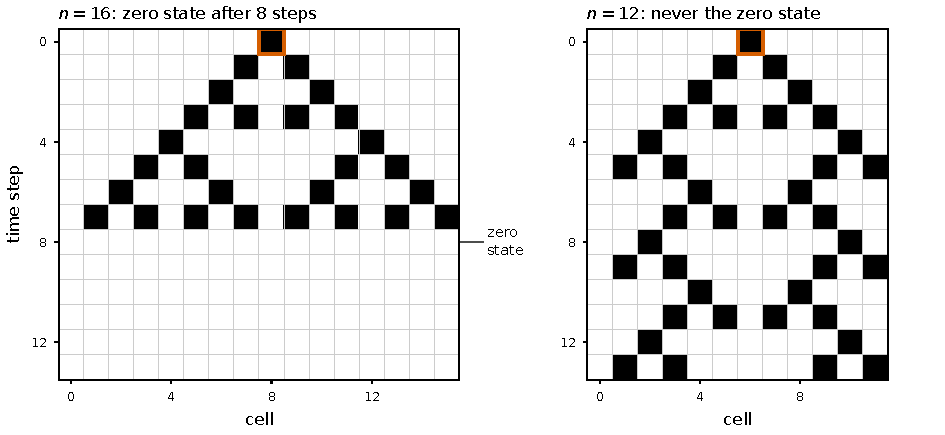
\includegraphics[width=0.78\textwidth]{figures/fig_zero_154.pdf}
\caption{Rule 154, one flip of the zero state (outlined cell); time runs downwards, black cells carry $1$. Left,
$n=16$: the orbit lies on one parity class at each time, where the rule acts as rule 90
(Lemma~\ref{154:lem:rule90}), and reaches the zero state after $n/2$ steps (Lemma~\ref{154:lem:nilpotent}(a)).
Right, $n=12$: the orbit never reaches the zero state (Lemma~\ref{154:lem:nilpotent}(b)) and ends on another cycle.
Simulated by \texttt{make\_figures.py}.}
\label{fig:154}
\end{figure}

\begin{lemma}[local form]\label{154:lem:local}
$f(a,b,c)=c+a(1+b)$, that is, $(Fx)_i=x_{i+1}+x_{i-1}(1+x_i)$.
\end{lemma}
\begin{proof}
On the codes $\code{000}$, $\code{001}$, $\code{010}$, $\code{011}$, $\code{100}$, $\code{101}$, $\code{110}$,
$\code{111}$ the right-hand side takes the values $0$, $1$, $0$, $1$, $1$, $0$, $0$, $1$.
\end{proof}

\begin{lemma}[rule 90 on the parity classes]\label{154:lem:rule90}
Let $n$ be even, $n\ge 4$. If $x\in E$, then $F(x)\in O$ and $(Fx)_i=x_{i-1}+x_{i+1}$ for all $i$; the same holds
with $E$ and $O$ exchanged. Hence $F^t(x)=L^tx$ for all $t\ge 0$ and all $x\in E\cup O$.
\end{lemma}
\begin{proof}
Let $x\in E$. For odd $i$, $x_i=0$ and Lemma~\ref{154:lem:local} gives $(Fx)_i=x_{i+1}+x_{i-1}$. For even $i$,
$x_{i-1}=x_{i+1}=0$, so $(Fx)_i=0=x_{i-1}+x_{i+1}$. Hence $F(x)=Lx$ and $F(x)\in O$. The case $x\in O$ is the same
with the parities exchanged, and the last statement follows by induction on $t$.
\end{proof}

\begin{lemma}[nilpotency on $E\cup O$]\label{154:lem:nilpotent}
\textup{(a)} If $n=2^k$, $k\ge 2$, then $F^{n/2}(x)=\zero$ for every $x\in E\cup O$.
\textup{(b)} If $n$ is even and not a power of two, then $F^t(e_j)\neq\zero$ for all $t\ge 0$ and all cells $j$.
\end{lemma}
\begin{proof}
By Lemma~\ref{154:lem:rule90}, $F^t(x)=L^tx$ on $E\cup O$. The rotation $\sigma$ generates a commutative algebra
over $\mathrm{GF}(2)$, so $L^{2^s}=\sigma^{2^s}+\sigma^{-2^s}$.
(a) For $2^s=n/2$: $L^{n/2}=\sigma^{-n/2}(\sigma^n+1)=0$.
(b) Identify $e_j$ with $z^j$ in $\mathrm{GF}(2)[z]/(z^n+1)$; then $L^te_0=z^{-t}(1+z)^{2t}$, which is $0$ if and
only if $z^n+1$ divides $(1+z)^{2t}$ in $\mathrm{GF}(2)[z]$. Write $n=2^aq$ with $q$ odd, $q\ge 3$. Then
$z^n+1=(z^q+1)^{2^a}$ and $z^q+1=(z+1)(1+z+\dots+z^{q-1})$. The second factor has the value $q\equiv 1\pmod 2$ at
$z=1$, so it is not divisible by $z+1$; it has degree $q-1\ge 2$ and therefore has an irreducible factor different
from $z+1$, which does not divide any power of $1+z$. By rotation the same holds for every $e_j$.
\end{proof}

For rule 90 itself, the statement that on a ring of $2^k$ cells every state reaches $\zero$ is Lemma~3.5 of
\cite{MartinOdlyzkoWolfram1984}, and the converse for a single $1$ follows from Theorems~3.3 and~3.4 there with their corollaries; the
proof is given here because Theorems~\ref{154:thm:pow2} and~\ref{154:thm:other} depend on it.

\begin{lemma}[invariance of $M$]\label{154:lem:invariant}
Let $n$ be even, $n\ge 4$. Then $F(M)\subseteq M$.
\end{lemma}
\begin{proof}
Let $x\in M$ and suppose $F(x)\in O$, that is, $(Fx)_i=0$ for every even $i$. By Lemma~\ref{154:lem:local},
$x_{i+1}=x_{i-1}(1+x_i)$ for every even $i$; with $j=i+1$ this reads $x_j=x_{j-2}(1+x_{j-1})\le x_{j-2}$ for every
odd $j$. The odd cells form one orbit of $j\mapsto j-2$ ($n$ is even), so going once around the ring gives
$x_j\le x_{j-2}\le\dots\le x_j$: all odd cells carry the same value. Since $x\in M$, some odd cell carries a $1$,
hence all do, and then $1=1\cdot(1+x_{j-1})$ for every odd $j$, that is, all even cells are $0$. This contradicts
$x\in M$. The case $F(x)\in E$ is the same with the parities exchanged.
\end{proof}

\begin{lemma}[collisions]\label{154:lem:collisions}
Let $n\ge 3$ and $F(x)=F(y)$ with $x\neq y$. Then $n$ is even and one of the following holds: $x,y\in E$ and
$x+y=\one_E$; or $x,y\in O$ and $x+y=\one_O$; or $\{x,y\}=\{\one_E,\one_O\}$. In particular, $F$ is a bijection when
$n$ is odd, and for even $n$ two different states with the same image both lie in $E\cup O$.
\end{lemma}
\begin{proof}
Put $d=x+y\neq\zero$. By Lemma~\ref{154:lem:local}, $(Fx)_i=(Fy)_i$ reads
\begin{equation}\label{154:eq:star}
d_{i+1}=x_{i-1}(1+x_i)+y_{i-1}(1+y_i)\qquad\text{for all } i .
\end{equation}
\begin{enumerate}[label=\textup{(\roman*)},nosep,leftmargin=2.2em]
\item If $d_{i-1}=d_i=0$, then $d_{i+1}=0$; hence, if $d$ had two cyclically consecutive zeros, $d$ would be
$\zero$. So $d$ has no two consecutive zeros.
\item If $d_{i-1}=1$ and $d_i=0$, then $x_i=y_i=:b$ and \eqref{154:eq:star} gives
$d_{i+1}=(1+b)(x_{i-1}+y_{i-1})=1+b$; by (i), $d_{i+1}=1$, so $x_i=y_i=0$.
\item If $d_{i-1}=0$ and $d_i=1$, then $x_{i-1}=y_{i-1}$ and \eqref{154:eq:star} gives
$d_{i+1}=x_{i-1}(x_i+y_i)=x_{i-1}$.
\item If $d_{i-1}=d_i=1$, then $y=1+x$ at both cells and \eqref{154:eq:star} gives
$d_{i+1}=x_{i-1}(1+x_i)+(1+x_{i-1})x_i=x_{i-1}+x_i$.
\end{enumerate}
\emph{Case A: $d_i=0$ for some $i$.} By (i), $d_{i-1}=d_{i+1}=1$; by (ii), $x_i=y_i=0$; by (iii) applied to the
pair of cells $(i,i+1)$, $d_{i+2}=x_i=0$. So the hypothesis of Case A holds again at $i+2$, and by induction
$d_{i+2s}=0$, $x_{i+2s}=y_{i+2s}=0$ and $d_{i+2s+1}=1$ for all $s$. If $n$ were odd, the cells $i+2s$ would exhaust
the ring and $d$ would be $\zero$; so $n$ is even, $x$ and $y$ vanish on the parity class of $i$ and differ at
every cell of the other class: both lie in $E$ (or both in $O$) and $x+y=\one_E$ (or $\one_O$).
\emph{Case B: $d$ has no zero.} Then $y=1+x$ at every cell and (iv) gives $x_{i-1}+x_i=1$ for all $i$: $x$
alternates, so $n$ is even and $\{x,y\}=\{\one_E,\one_O\}$.
\end{proof}

That rule 154 is a bijection on rings of odd size is known: it is stated in \cite{BhattacharjeeDas2019} and in
\cite{Fedoriaka2025} and, according to its abstract, in \cite{NobeYura2004}, which was not read.

\begin{lemma}[periodic states]\label{154:lem:periodic}
Let $n$ be even, $n\ge 4$. The restriction of $F$ to $M$ is a permutation of $M$, and every state of $M$ is
periodic. The periodic states of $F$ are the states of $M$ and the periodic states of $L$ in $E\cup O$. If $n=2^k$,
$k\ge 2$, the periodic states are exactly the states of $M\cup\{\zero\}$, and the cycles are $\{\zero\}$ and the
cycles contained in $M$.
\end{lemma}
\begin{proof}
$F$ maps $M$ into $M$ (Lemma~\ref{154:lem:invariant}) and is injective on $M$ (Lemma~\ref{154:lem:collisions}: two
different states with the same image lie in $E\cup O$). An injective map of a finite set into itself is a
permutation, so every $x\in M$ satisfies $F^t(x)=x$ for some $t\ge 1$. $E\cup O$ is mapped into itself, and
$F=L$ there (Lemma~\ref{154:lem:rule90}). For $n=2^k$ every state of $E\cup O$ reaches $\zero$
(Lemma~\ref{154:lem:nilpotent}(a)), so $\zero$ is the only periodic state outside $M$. A cycle that meets $M$ stays
in $M$ (Lemma~\ref{154:lem:invariant}).
\end{proof}

\begin{lemma}[one-flip moves]\label{154:lem:moves}
Let $n$ be even, $n\ge 4$, let $C$ be a cycle contained in $M$, $x\in C$, $j$ a cell and $y=x+e_j$.
\begin{enumerate}[label=\textup{(\alph*)},nosep,leftmargin=2.2em]
\item If $y\in M$, then $y$ lies on a cycle $C_y\subseteq M$, and either $C_y=C$ or both $C\to C_y$ and
$C_y\to C$ are edges of $\Gone$.
\item Any two cycles contained in $M$ are joined, in both directions, by a directed path of $\Gone$ through cycles
contained in $M$.
\end{enumerate}
\end{lemma}
\begin{proof}
(a) By Lemma~\ref{154:lem:periodic}, $y$ is periodic and its cycle $C_y$ is contained in $M$. If $C_y\neq C$, then
$x$ and $y=x+e_j$ are periodic states of the different cycles $C$ and $C_y$, and Lemma~\ref{lem:edge} gives both
edges.
(b) From any $x\in M$ one reaches $\one$ by setting the zeros of $x$ to $1$, one at a time; all intermediate states
contain the ones of $x$ and are in $M$. By (a), consecutive states lie on equal cycles or on cycles joined by edges
of $\Gone$ in both directions. So every cycle contained in $M$ is joined in both directions to the cycle $\{\one\}$
($F(\one)=\one$).
\end{proof}

\begin{theorem}[$n$ a power of two]\label{154:thm:pow2}
Let $n=2^k$, $k\ge 2$.
\begin{enumerate}[label=\textup{(\alph*)},nosep,leftmargin=2.2em]
\item The cycles are $\{\zero\}$ and the cycles contained in $M$.
\item No edge of $\Gone$ leaves $\{\zero\}$: $V(\{\zero\},C)\ge 2$ for every cycle $C\neq\{\zero\}$.
\item Every cycle $C\neq\{\zero\}$ has a directed path in $\Gone$ to $\{\zero\}$, of length at most
$\mu(C)\le n/2$, where $\mu(C):=\min_{x\in C}\min(|x|_E,|x|_O)$.
\item $\{\zero\}$ is the only closed class of $\Gone$.
\item $\gamma(\{\zero\})=m-1$ and $\gamma(C)=m$ for every cycle $C\neq\{\zero\}$; hence $\Sel=\{\{\zero\}\}$.
\item $k_{\code{000}}=0$ and $k_v=1$ for each of the seven codes $v\neq\code{000}$; hence $\kst=1$.
\end{enumerate}
\end{theorem}
\begin{proof}
(a) Lemma~\ref{154:lem:periodic}.

(b) By Lemma~\ref{lem:edge}, an edge $\{\zero\}\to C$ requires a cell $j$ such that the orbit of
$\zero+e_j=e_j$ ends on $C$. The state $e_j$ lies in $E\cup O$, so by Lemmas~\ref{154:lem:rule90}
and~\ref{154:lem:nilpotent}(a) its orbit stays in $E\cup O$ and reaches $\zero$ after at most $n/2$ steps; by (a)
none of its states lies on a cycle other than $\{\zero\}$. So no orbit of a single flip of $\zero$ ends on another
cycle.

(c) Choose $x\in C$ attaining $\mu=\mu(C)$. Since $x\in M$, $\mu\ge 1$. Assume $|x|_O\le|x|_E$ (otherwise exchange
the parities) and let $j_1,\dots,j_\mu$ be the odd cells of $x$ that carry a $1$. Put $x^{(0)}=x$ and
$x^{(s)}=x^{(s-1)}+e_{j_s}$. For $s<\mu$, $x^{(s)}$ still has a $1$ on an odd cell and has all the ones of $x$ on
even cells, so $x^{(s)}\in M$ lies on a cycle $C_s\subseteq M$ (Lemma~\ref{154:lem:periodic}), and $C_0=C$. For
$s<\mu-1$, Lemma~\ref{154:lem:moves}(a), applied to $x^{(s)}$ and the cell $j_{s+1}$, shows that $C_{s+1}=C_s$ or
$C_s\to C_{s+1}$ is an edge of $\Gone$. Finally $x^{(\mu)}=x^{(\mu-1)}+e_{j_\mu}$ lies in $E\setminus\{\zero\}$ and
its orbit ends in $\zero$ (Lemma~\ref{154:lem:nilpotent}(a)); by Lemma~\ref{lem:edge}, $C_{\mu-1}\to\{\zero\}$ is an
edge. After deleting repetitions, $C=C_0,C_1,\dots,C_{\mu-1},\{\zero\}$ is a directed path in $\Gone$ of length at
most $\mu\le n/2$.

(d) By (c) every strongly connected component other than $\{\zero\}$ has an outgoing edge; by (b) $\{\zero\}$ has
none.

(e) Every spanning in-tree has $m-1$ edges, each of weight at least $1$ (Lemma~\ref{lem:edge}). By (c) each cycle
$C\neq\{\zero\}$ has an edge of $\Gone$ to a cycle with a smaller distance to $\{\zero\}$ in $\Gone$; these $m-1$
edges form an in-tree rooted at $\{\zero\}$ of weight $m-1$, so $\gamma(\{\zero\})=m-1$. Let $C\neq\{\zero\}$. An
in-tree rooted at $C$ contains one edge that leaves $\{\zero\}$, of weight at least $2$ by (b), so
$\gamma(C)\ge(m-2)+2=m$. Conversely, let $C_*$ be the cycle of $e_0+e_1$, a state of $M$. The step from $\zero$ to
$F(\zero)+e_0+e_1$ has resistance $2$, so $V(\{\zero\},C_*)\le 2$. By Lemma~\ref{154:lem:moves}(b) the $m-1$ cycles
contained in $M$ have a spanning in-tree rooted at $C$ all of whose edges are edges of $\Gone$ (weight $m-2$);
adding the edge $\{\zero\}\to C_*$ gives an in-tree rooted at $C$ of weight $m$. Hence
$\gamma(C)=m>\gamma(\{\zero\})$.

(f) $k_{\code{000}}=0$ because $\{\zero\}$ is selected and $\zero$ contains the code $\code{000}$
(Lemma~\ref{lem:kzero}). Let
$v\neq\code{000}$. For $C=\{\zero\}$, $\gamma(C)=m-1$ and $R(\{\zero\}\to\Dc{v})\ge 1$, since $\zero\notin\Dc{v}$;
for $C\neq\{\zero\}$, $\gamma(C)=m$. So $k_v\ge 1$. For the upper bounds, $e_0$ contains the codes $\code{001}$,
$\code{010}$, $\code{100}$ (at the cells $-1$, $0$, $1$), and $F(e_0)=e_{-1}+e_1$ (Lemma~\ref{154:lem:rule90})
contains the code $\code{101}$ at the cell $0$ ($n\ge 4$); both states are reached from $\{\zero\}$ with resistance
$1$, so $k_v\le 1$ for these four codes. The state $e_0+e_1$ is in $M$, hence on a cycle with $\gamma=m$, and
contains the code $\code{011}$ at the cell $0$ and the code $\code{110}$ at the cell $1$; the cycle $\{\one\}$ has
$\gamma=m$ and contains the code $\code{111}$. So $k_v\le 1$ for these three codes.
\end{proof}

\begin{theorem}[all other $n$]\label{154:thm:other}
Let $n\ge 3$ not be a power of two. Then $\Gone$ is strongly connected, $\gamma(C)=m-1$ for every cycle $C$, all
cycles are selected, $k_v=0$ for all eight codes $v$, and $\kst=0$.
\end{theorem}
\begin{proof}
\emph{$n$ odd.} $F$ is a bijection (Lemma~\ref{154:lem:collisions}), so every state is periodic, and a single flip
of a state $x$ of a cycle $C$ gives a state $y$ on a cycle $C_y$; by the last sentence of Lemma~\ref{lem:edge}, $C_y=C$ or
$C\to C_y$ and $C_y\to C$ are edges. Any two states are joined by a sequence of single flips, so $\Gone$ is strongly
connected.

\emph{$n$ even ($n\ge 6$).} The cycles are those contained in $M$ and those contained in $E\cup O$
(Lemma~\ref{154:lem:periodic}).
(1) The cycles contained in $M$ are mutually reachable (Lemma~\ref{154:lem:moves}(b)).
(2) Let $C\subseteq E\cup O$ be a cycle other than $\{\zero\}$ and $x\in C$, $x\neq\zero$, say $x\in E$. For an odd
cell $j$, $y=x+e_j$ is in $M$, hence on a cycle $C_y\subseteq M$; $C\to C_y$ is an edge (Lemma~\ref{lem:edge}), and
so is $C_y\to C$, because $y+e_j=x$ lies on $C$.
(3) A single flip of $\zero$ gives a state $e_j$, whose orbit stays in $E\cup O$ (Lemma~\ref{154:lem:rule90}) and
never reaches $\zero$ (Lemma~\ref{154:lem:nilpotent}(b)); it ends on a cycle $C_1\subseteq E\cup O$,
$C_1\neq\{\zero\}$, so $\{\zero\}\to C_1$ is an edge, and from $C_1$ the cycles in $M$ are reached by (2). In the
other direction, $y=\one_E+e_1$ is in $M$, $y+e_1=\one_E$ and $F(\one_E)=L\one_E=\zero$, so $C_y\to\{\zero\}$ is an
edge. By (1)--(3), $\Gone$ is strongly connected.

In both cases every cycle is the root of a spanning in-tree of edges of $\Gone$, so $\gamma=m-1$ for all cycles and
all are selected. All eight codes occur on periodic states: $\code{000}$ on $\zero$; $\code{111}$ on $\one$; for
$n\ge 5$ the codes $\code{001}$, $\code{011}$, $\code{100}$, $\code{110}$ on $\code{0}^{n-2}\code{11}$ and the codes
$\code{010}$, $\code{101}$ on $\code{0}^{n-4}\code{1011}$ (both states are in $M$ for even $n$ and periodic for odd
$n$); for $n=3$ the states $\code{001}$ and $\code{011}$ contain the codes $\code{001}$, $\code{010}$, $\code{100}$
and $\code{011}$, $\code{101}$, $\code{110}$. Hence $k_v=0$ for all $v$ (Lemma~\ref{lem:kzero}).
\end{proof}

\begin{theorem}\label{154:thm:main}
For rule 154 and every $n\ge 3$: $\kst=1$ if $n$ is a power of two ($n\ge 4$), and $\kst=0$ otherwise. In the first
case $\Sel=\{\{\zero\}\}$, $k_{\code{000}}=0$ and $k_v=1$ for the seven other codes $v$; in the second case $\Sel$
is the set of all cycles and $k_v=0$ for all eight codes $v$.
\end{theorem}
\begin{proof}
Theorems~\ref{154:thm:pow2} and~\ref{154:thm:other}.
\end{proof}

\subsection{Rules 43 and 142}\label{sec:43}

In this section $F$ is the global map of rule~43 or of rule~142, and $n\ge 3$ unless a range is stated. The two
local rules are
\[
\begin{array}{l|cccccccc}
abc & \code{000}&\code{001}&\code{010}&\code{011}&\code{100}&\code{101}&\code{110}&\code{111}\\ \hline
\text{rule 142: } f(a,b,c) & 0&1&1&1&0&0&0&1\\
\text{rule 43: } f(a,b,c) & 1&1&0&1&0&1&0&0
\end{array}
\]

\begin{lemma}[common form]\label{43:lem:R}
For both rules $f(a,b,c)=c$ if $a\ne c$. If $a=c$, then $f(a,b,c)=b$ for rule~142 and $f(a,b,c)=1-b$ for
rule~43.
\end{lemma}
\begin{proof}
On the codes $\code{001}$, $\code{011}$, $\code{100}$, $\code{110}$ both rows of the table read $1,1,0,0$,
which is $c$. On $\code{000}$, $\code{010}$, $\code{101}$, $\code{111}$ the row of rule~142 reads $0,1,0,1$, which
is $b$, and the row of rule~43 reads $1,0,1,0$, which is $1-b$.
\end{proof}

\paragraph{Walls.}
The \emph{wall word} of a state $x$ is $\delta(x)\in\st$ with $\delta(x)_i=x_i+x_{i+1}$: there is a wall between
the cells $i$ and $i+1$ iff $\delta(x)_i=1$. The \emph{wall count} is $w(x)=|\delta(x)|$. It is even, because mod~2 the
sum of the $\delta(x)_i$ is twice the sum of the $x_i$. Further $\delta(\cpl{x})=\delta(x)$. A flip toggles the two walls next to the flipped cell:
\begin{equation}\label{43:eq:flip}
\delta(x+e_j)=\delta(x)+e_{j-1}+e_j .
\end{equation}
Cell $j$ of $x$ is \emph{isolated} if it differs from both neighbours and \emph{interior} if it equals both
neighbours. For a word $d\in\st$ let
\[
P(d)=\{i: d_i=d_{i+1}=1\},\qquad Q(d)=\{i: d_i=d_{i+1}=0\},
\]
so that cell $j$ of $x$ is isolated iff $j-1\in P(\delta(x))$ and interior iff $j-1\in Q(\delta(x))$. A
\emph{run} is a maximal block of equal cells. In a non-constant state the isolated cells are the runs of length~1,
and there is an interior cell iff there is a run of length at least~3. Let $G_{184}$ and $G_{226}$ be the global
maps on $\st$ of the local rules
\[
g_{184}(a,b,c)=1 \text{ iff } (b,c)=(1,1) \text{ or } (a,b)=(1,0),\qquad
g_{226}(a,b,c)=1 \text{ iff } (a,b)=(1,1) \text{ or } (b,c)=(0,1).
\]
Since $g_{226}(a,b,c)=g_{184}(c,b,a)$, we have $G_{226}=\rho\,G_{184}\,\rho$.

\begin{lemma}[wall map]\label{43:lem:wall}
Let $d=\delta(x)$. For rule~142, $(Fx)_i=x_i+d_i(1+d_{i-1})$ and $\delta(Fx)=G_{226}(\delta(x))$. For rule~43,
$(Fx)_i=x_i+1+d_{i-1}(1+d_i)$ and $\delta(Fx)=G_{184}(\delta(x))$.
\end{lemma}
\begin{proof}
$x_{i-1}\ne x_{i+1}$ iff $d_{i-1}+d_i=1$.
\emph{Rule 142.} By Lemma~\ref{43:lem:R}, $(Fx)_i=x_{i+1}=x_i+d_i$ if $d_{i-1}+d_i=1$ and $(Fx)_i=x_i$
otherwise. So $(Fx)_i=x_i+d_i(d_{i-1}+d_i)=x_i+d_i(1+d_{i-1})$, using $d_id_i=d_i$. Then
$\delta(Fx)_i=(Fx)_i+(Fx)_{i+1}=d_i+d_i(1+d_{i-1})+d_{i+1}(1+d_i)=d_{i-1}d_i+(1+d_i)d_{i+1}$. The two terms
exclude each other; the sum is $1$ iff $(d_{i-1},d_i)=(1,1)$ or $(d_i,d_{i+1})=(0,1)$, which is $g_{226}$.
\emph{Rule 43.} By Lemma~\ref{43:lem:R}, $(Fx)_i=x_i+d_i$ if $d_{i-1}+d_i=1$ and $(Fx)_i=x_i+1$ otherwise. The
change $(Fx)_i+x_i$ is $1,1,1,0$ for $(d_{i-1},d_i)=(0,0),(1,1),(0,1),(1,0)$, that is, $1+d_{i-1}(1+d_i)$. The
two constants $1$ of the cells $i$ and $i+1$ cancel, so
$\delta(Fx)_i=d_i+d_{i-1}(1+d_i)+d_i(1+d_{i+1})=d_id_{i+1}+d_{i-1}(1+d_i)$, which is $1$ iff
$(d_i,d_{i+1})=(1,1)$ or $(d_{i-1},d_i)=(1,0)$: this is $g_{184}$.
\end{proof}

\begin{lemma}[conservation]\label{43:lem:cons}
(a) $|G_{184}(d)|=|d|$ and $|G_{226}(d)|=|d|$ for every word $d$.
(b) For both rules $F(\cpl{x})=\cpl{F(x)}$ and $w(Fx)=w(x)$. Hence the wall count is constant along every orbit;
it is an even number $w(C)$ attached to each cycle $C$.
\end{lemma}
\begin{proof}
(a) As integers, $(G_{184}d)_i=d_id_{i+1}+d_{i-1}(1-d_i)$, because the two terms exclude each other. Summing over
the ring gives $\sum_i d_id_{i+1}+\sum_i d_{i-1}-\sum_i d_{i-1}d_i=\sum_i d_i$. Rule~226 is the reflection.
(b) The form of Lemma~\ref{43:lem:R} is unchanged when $a$, $b$, $c$ and the value are complemented together
($a\ne c$ is preserved; $c$ becomes $1-c$; $b$ becomes $1-b$ and $1-b$ becomes $b$). By
Lemma~\ref{43:lem:wall} and (a), $w(Fx)=|\delta(Fx)|=|G(\delta(x))|=|\delta(x)|$ with $G=G_{184}$ or $G_{226}$.
\end{proof}

Lemma~\ref{43:lem:wall} and the conservation of the wall count are known. Up to a shift of the indices,
$\delta$ is the local map of rule~60; that it transforms rule~43 into rule~184 and rule~142 into rule~226, and
that both rules conserve the number of blocks $\code{10}$, which is $w(x)/2$, is stated in
\cite{Fuks2005,Fuks2005b} (in Fuk\'s's paper on rule~142 for that rule only), where the two identities are
credited to \cite{Boccara1993}.

\begin{lemma}[flip]\label{43:lem:flip}
$w(x+e_j)-w(x)$ is $+2$ if cell $j$ of $x$ is interior, $-2$ if it is isolated, and $0$ otherwise.
\end{lemma}
\begin{proof}
By \eqref{43:eq:flip} the flip toggles $\delta(x)_{j-1}$ and $\delta(x)_j$, two different positions as $n\ge 2$.
\end{proof}

\begin{lemma}[pairs]\label{43:lem:pairs}
Let $d$ be a word.
\begin{enumerate}[label=(\alph*),nosep,leftmargin=*]
\item Let $d'=G_{184}(d)$ and $N(d)=\{i\in Q(d): i+2\in P(d)\}$. Then
$i\in P(d')$ iff $i+1\in P(d)$ and $i-1\notin Q(d)$; and $i\in Q(d')$ iff $i-1\in Q(d)$ and $i+1\notin P(d)$.
Hence $|P(d')|=|P(d)|-|N(d)|$ and $|Q(d')|=|Q(d)|-|N(d)|$, and if $N(d)=\emptyset$ then $P(d')=P(d)-1$ and
$Q(d')=Q(d)+1$.
\item Let $d'=G_{226}(d)$ and $N'(d)=\{i\in P(d): i+2\in Q(d)\}$. Then
$i\in P(d')$ iff $i-1\in P(d)$ and $i+1\notin Q(d)$; and $i\in Q(d')$ iff $i+1\in Q(d)$ and $i-1\notin P(d)$.
Hence $|P(d')|=|P(d)|-|N'(d)|$ and $|Q(d')|=|Q(d)|-|N'(d)|$, and if $N'(d)=\emptyset$ then $P(d')=P(d)+1$,
$Q(d')=Q(d)-1$.
\item $|P(d)|-|Q(d)|=2|d|-n$.
\end{enumerate}
\end{lemma}
\begin{proof}
(a) $d'_i=1$ iff $[d_i=d_{i+1}=1]$ or $[d_{i-1}=1,\ d_i=0]$. Let $d'_i=d'_{i+1}=1$. Of the four combinations of
a bracket for $i$ with a bracket for $i+1$, two are contradictory ($[d_i=d_{i+1}=1]$ with $[d_i=1,\ d_{i+1}=0]$;
$[d_{i-1}=1,\ d_i=0]$ with $[d_i=1,\ d_{i+1}=0]$). The other two are $d_i=d_{i+1}=d_{i+2}=1$, and
$d_{i-1}=1$, $d_i=0$, $d_{i+1}=d_{i+2}=1$. Together: $d_{i+1}=d_{i+2}=1$ and not $d_{i-1}=d_i=0$. This is the
first equivalence. Going through $d_i=1$ and $d_i=0$ one finds $d'_i=0$ iff $[d_i=1,\ d_{i+1}=0]$ or
$[d_{i-1}=d_i=0]$. Let $d'_i=d'_{i+1}=0$. Two combinations are contradictory ($[d_i=1,\ d_{i+1}=0]$ with
$[d_{i+1}=1,\ d_{i+2}=0]$; $[d_i=1,\ d_{i+1}=0]$ with $[d_i=d_{i+1}=0]$). The other two are $d_{i-1}=d_i=0$,
$d_{i+1}=1$, $d_{i+2}=0$, and $d_{i-1}=d_i=d_{i+1}=0$. Together: $d_{i-1}=d_i=0$ and not $d_{i+1}=d_{i+2}=1$.
This is the second equivalence. Both are statements about the values $d_{i-1},\dots,d_{i+2}$ and remain true when
some of these cells coincide ($n=3$). Counting: $P(d')$ is the set of $i$ with $i+1\in P(d)$, minus those with in
addition $i-1\in Q(d)$; the latter correspond to the elements $i-1$ of $N(d)$. The count for $Q(d')$ is the same.
If $N(d)=\emptyset$, the side conditions never fail.

(b) Apply (a) to $\rho d$, using $G_{226}=\rho\,G_{184}\,\rho$, $P(\rho d)=-P(d)-1$ and $Q(\rho d)=-Q(d)-1$:
$i\in P(G_{226}d)$ iff $-i-1\in P(G_{184}\rho d)$ iff [$-i\in P(\rho d)$ and $-i-2\notin Q(\rho d)$] iff
[$i-1\in P(d)$ and $i+1\notin Q(d)$]; likewise for $Q$. The pattern $\code{0011}$ counted by $N$ is reflected
into the pattern $\code{1100}$ counted by $N'$.

(c) Every $1$ of $d$ is followed by a $1$ or by a $0$: $|d|=|P(d)|+\#\{i:(d_i,d_{i+1})=(1,0)\}$. Every $0$ is
followed by a $0$ or by a $1$: $n-|d|=|Q(d)|+\#\{i:(d_i,d_{i+1})=(0,1)\}$. On a ring the numbers of blocks
$\code{10}$ and $\code{01}$ are equal. Subtract.
\end{proof}

\begin{lemma}[periodic wall words]\label{43:lem:pww}
For $G=G_{184}$ and for $G=G_{226}$, a word $d$ is periodic under $G$ iff $P(d)=\emptyset$ or $Q(d)=\emptyset$.
Moreover, $G_{184}d=\sigma d$ and $G_{226}d=\sigma^{-1}d$ if $P(d)=\emptyset$, and $G_{184}d=\sigma^{-1}d$ and
$G_{226}d=\sigma d$ if $Q(d)=\emptyset$.
\end{lemma}
\begin{proof}
\emph{Rule 184.} If $P(d)=\emptyset$, then $d_id_{i+1}=0$ and $d_{i-1}d_i=0$ for all $i$, so
$(Gd)_i=d_id_{i+1}+d_{i-1}(1-d_i)=d_{i-1}$. If $Q(d)=\emptyset$: for $d_i=1$, $(Gd)_i=d_{i+1}$; for $d_i=0$,
$d_{i-1}=d_{i+1}=1$ and $(Gd)_i=1=d_{i+1}$. In both cases $Gd$ is a rotation of $d$, so $P$ or $Q$ is empty
again, and $G^nd=d$.
Conversely let $G^{t_0}d=d$ with $t_0\ge 1$. By Lemma~\ref{43:lem:pairs}(a), $|P(G^td)|$ does not increase with
$t$ and is periodic in $t$, hence constant. So $N(G^td)=\emptyset$ for all $t\ge 0$, and therefore
$P(G^td)=P(d)-t$ and $Q(G^td)=Q(d)+t$. Suppose $p\in P(d)$ and $q\in Q(d)$. Let $g\in\{1,\dots,n\}$ with
$g=p-q$ mod $n$, and $t=\lfloor (g-1)/2\rfloor\ge 0$; then $g-2t$ is $1$ or $2$. Put
$p'=p-t\in P(G^td)$ and $q'=q+t\in Q(G^td)$, so that $p'-q'=g-2t$ mod $n$. If $g-2t=1$, the cell $q'+1=p'$ of
$G^td$ carries $0$ (as $q'\in Q$) and $1$ (as $p'\in P$): impossible. If $g-2t=2$, then $q'\in N(G^td)$, which is
empty: impossible. So $P(d)$ or $Q(d)$ is empty.
\emph{Rule 226.} $d$ is periodic under $G_{226}$ iff $\rho d$ is periodic under $G_{184}$ iff $P(\rho d)$ or
$Q(\rho d)$ is empty iff $P(d)$ or $Q(d)$ is empty; and $\rho\sigma\rho=\sigma^{-1}$.
\end{proof}

\begin{lemma}[periodic states]\label{43:lem:per}
For both rules:
\begin{enumerate}[label=(\alph*),nosep,leftmargin=*]
\item a state is periodic iff it has no isolated cell or no interior cell;
\item for rule~43, $Fx=\cpl{\sigma x}$ if $x$ has no isolated cell and $Fx=\sigma^{-1}x$ if $x$ has no interior
cell; for rule~142, $Fx=\sigma^{-1}x$ if $x$ has no isolated cell and $Fx=\cpl{\sigma x}$ if $x$ has no interior
cell; each of the two properties is preserved by $F$, by $\sigma$ and by the complement;
\item if $u$ is periodic and $s$ is an integer, then $\sigma^su$ lies on the cycle of $u$ or on the cycle of
$\cpl{u}$.
\end{enumerate}
\end{lemma}
\begin{proof}
(b) Let $d=\delta(x)$. No isolated cell means $P(d)=\emptyset$, that is, $d_{i-1}d_i=0$ for all $i$; no interior
cell means $Q(d)=\emptyset$, that is, $(1+d_{i-1})(1+d_i)=0$ for all $i$. Insert this into
Lemma~\ref{43:lem:wall}.
Rule~43, $P(d)=\emptyset$: $(Fx)_i=x_i+1+d_{i-1}=1+x_{i-1}$.
Rule~43, $Q(d)=\emptyset$: $d_{i-1}(1+d_i)=1+d_i$ (if $d_i=0$ then $d_{i-1}=1$), so $(Fx)_i=x_i+1+1+d_i=x_{i+1}$.
Rule~142, $P(d)=\emptyset$: $d_i(1+d_{i-1})=d_i$, so $(Fx)_i=x_i+d_i=x_{i+1}$.
Rule~142, $Q(d)=\emptyset$: $d_i(1+d_{i-1})=1+d_{i-1}$ (if $d_{i-1}=0$ then $d_i=1$), so
$(Fx)_i=x_i+1+x_{i-1}+x_i=1+x_{i-1}$.
The rotation and the complement map isolated cells to isolated cells and interior cells to interior cells, so
both properties are preserved.

(a) By (b) the formulas apply to every $F^tx$, and $F^{2n}x=x$: $x$ is periodic. Conversely, if $F^{t_0}x=x$ with
$t_0\ge 1$, then $G^{t_0}(\delta(x))=\delta(F^{t_0}x)=\delta(x)$ by Lemma~\ref{43:lem:wall}, so
$P(\delta(x))$ or $Q(\delta(x))$ is empty by Lemma~\ref{43:lem:pww}.

(c) If $F$ acts as $\sigma^{-1}$ on the states with the property of $u$, then $\sigma^su=F^tu$ for any $t\ge 0$
with $t=-s$ mod $n$. If $F$ acts as $x\mapsto\cpl{\sigma x}$, then $F^tu$ is $\sigma^tu$ for even $t$ and
$\cpl{\sigma^tu}$ for odd $t$; so for $t\ge 0$ with $t=s$ mod $2n$, $\sigma^su$ is $F^tu$ for even $s$ and
$\cpl{F^tu}$ for odd $s$. The first lies on the cycle of $u$, the second on the cycle of $\cpl{u}$, which is the
complement of the cycle of $u$ by Lemma~\ref{43:lem:cons}(b).
\end{proof}

\paragraph{Rings with $4\mid n$.}
For $4\mid n$ let $\hat x=(\code{0011})^{n/4}$ (the cells $0,1$ carry $0$, the cells $2,3$ carry $1$, and so on)
and let $X$ be the set of the four rotations of $\hat x$.

\begin{lemma}[the level $n/2$]\label{43:lem:half}
Let $n$ be even. A state $x$ with $P(\delta(x))=Q(\delta(x))=\emptyset$ exists only if $4\mid n$, and these
states are then the four states of $X$. If $4\mid n$, the periodic states with wall count $n/2$ are exactly the
four states of $X$; they form one cycle, on which $F=\sigma^{-1}$, and they contain only the codes
$\code{001}$, $\code{011}$, $\code{110}$, $\code{100}$.
\end{lemma}
\begin{proof}
Let $d=\delta(x)$ with $P(d)=Q(d)=\emptyset$, that is, $d$ alternates: $d=(\code{01})^{n/2}$ or
$(\code{10})^{n/2}$. From $x_{i+1}=x_i+d_i$, $x$ is $aabbaabb\ldots$ or $abbaabba\ldots$ with $b=1-a$, which
closes up on the ring iff $n/2$ is even. These are the four rotations of $\hat x$.
Let $4\mid n$, let $x$ be periodic with $w(x)=n/2$, and $d=\delta(x)$. By Lemma~\ref{43:lem:pairs}(c),
$|P(d)|=|Q(d)|$; by Lemma~\ref{43:lem:per}(a) one of the two sets is empty; so both are, and $x\in X$.
In a state of $X$ each cell has exactly one equal neighbour (its wall word alternates), so only the codes
$\code{001}$, $\code{011}$, $\code{110}$, $\code{100}$ occur. On them $f(a,b,c)=c$ by Lemma~\ref{43:lem:R}, so $F=\sigma^{-1}$ on $X$, which
permutes the four states cyclically.
\end{proof}

\begin{theorem}\label{43:thm:crystal}
Let $n\ge 4$ and $4\mid n$. For both rules:
\begin{enumerate}[label=(\arabic*),nosep,leftmargin=*]
\item $X$ is a cycle of length $4$, and for every state $x$ of $X$ and every cell $j$ the orbit of $x+e_j$ ends
on $X$. Hence no edge of $\Gone$ leaves $X$, and $V(X,C')\ge 2$ for every cycle $C'\ne X$.
\item Every cycle $C\ne X$ has a directed path to $X$ in $\Gone$ with exactly $|w(C)-n/2|/2$ edges; along the
path the wall count moves by $2$ per edge towards $n/2$.
\item $\{X\}$ is the only closed class of $\Gone$.
\end{enumerate}
\end{theorem}
\begin{proof}
(1) $X$ is a cycle of length $4$ by Lemma~\ref{43:lem:half}. Let $x\in X$ and let $j$ be a cell. In $x$ every
cell has exactly one equal neighbour, so cell $j$ is neither interior nor isolated, and $w(x+e_j)=n/2$ by
Lemma~\ref{43:lem:flip}. The wall count is constant along the orbit (Lemma~\ref{43:lem:cons}), so the cycle on
which the orbit of $x+e_j$ ends consists of periodic states with wall count $n/2$. By Lemma~\ref{43:lem:half}
these are states of $X$, and a cycle contained in $X$ is $X$. So no single flip of a state of $X$ leads to
another cycle; the rest is Lemma~\ref{lem:edge}.

(2) Let $C\ne X$ be a cycle and $w=w(C)$. By Lemma~\ref{43:lem:half}, $w\ne n/2$; $w$ is even
(Lemma~\ref{43:lem:cons}) and so is $n/2$. Let $x\in C$ and $d=\delta(x)$. If $w<n/2$, then
$|P(d)|-|Q(d)|=2w-n<0$ by Lemma~\ref{43:lem:pairs}(c), so $Q(d)\ne\emptyset$: $x$ has an interior cell $j$, and
$w(x+e_j)=w+2$ (Lemma~\ref{43:lem:flip}). The orbit of $x+e_j$ ends on a cycle $C'$ with $w(C')=w+2$
(Lemma~\ref{43:lem:cons}), and $C'\ne C$ because the wall counts differ. So $C\to C'$ is an edge of $\Gone$
(Lemma~\ref{lem:edge}). If $w>n/2$, then $P(d)\ne\emptyset$, $x$ has an isolated cell $j$, and in the same way
$C\to C'$ with $w(C')=w-2$. Repeating this $|w-n/2|/2$ times gives a cycle with wall count $n/2$, which is $X$ by
Lemma~\ref{43:lem:half}.

(3) Let $K$ be a closed class. If $K$ contains a cycle $C\ne X$, the path of (2) from $C$ to $X$ stays in $K$, so
$X\in K$; $K$ is strongly connected and no edge leaves $X$, so $K=\{X\}$, a contradiction.
\end{proof}

\begin{corollary}\label{43:cor:div}
Let $n\ge 4$, $4\mid n$. For both rules $\Sel=\{X\}$ and $\gmin=m-1$; $k_v=0$ for
$v\in\{\code{001},\code{011},\code{100},\code{110}\}$ and $k_v=1$ for
$v\in\{\code{000},\code{010},\code{101},\code{111}\}$; and $\kst=1$.
\end{corollary}
\begin{proof}
By Theorem~\ref{43:thm:crystal}(3) the unique closed class is $\{X\}$, so $\Sel=\{X\}$ and $\gmin=m-1$ by
Theorem~\ref{thm:A}. By Lemma~\ref{lem:kzero}, $k_v=0$ iff $v$ occurs in a state of a selected cycle. The
states of $X$ contain only the codes $\code{001}$, $\code{011}$, $\code{100}$, $\code{110}$
(Lemma~\ref{43:lem:half}), and each of them occurs: in $\hat x$, $\code{100}$ at cell $0$, $\code{001}$ at
cell~$1$, $\code{011}$ at cell~$2$, $\code{110}$ at cell~$3$. So $k_v=0$ for these four codes, and $k_v\ge 1$ for
the other four, because $k_v$ is a non-negative integer.
Upper bound. The state $y=\hat x+e_2$ carries $0,0,0,1,0$ on the cells $0,\dots,4$ (cell $4$ is cell $0$ for
$n=4$): code $\code{000}$ at cell~$1$ and code $\code{010}$ at cell~$3$. The state $y'=\hat x+e_1$ carries
$1,0,1,1,1$ on the cells $n-1,0,1,2,3$: code $\code{101}$ at cell~$0$ and code $\code{111}$ at cell~$2$. Since
$F\sigma\hat x=\hat x$, the step from the state $\sigma\hat x$ of $X$ to $y$ has resistance
$H(F\sigma\hat x,y)=1$, and likewise for $y'$. So $R(X\to\Dc{v})\le 1$ and $k_v\le\gamma(X)+1-\gmin=1$ for
$v\in\{\code{000},\code{010},\code{101},\code{111}\}$.
\end{proof}


\begin{figure}[t]
\centering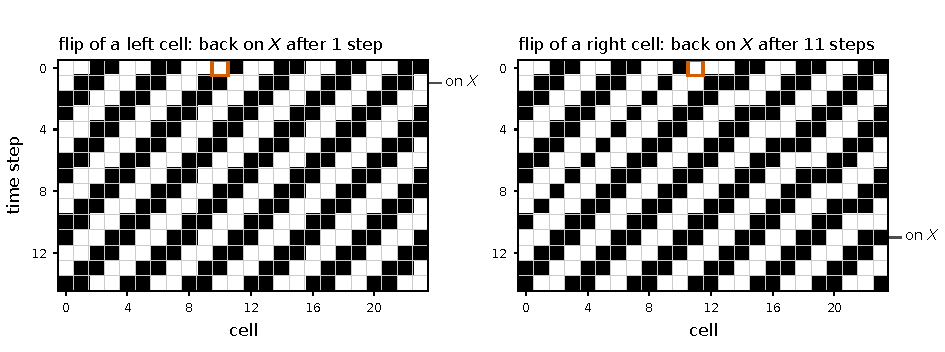
\includegraphics[width=0.84\textwidth]{figures/fig_crystal_43.pdf}
\caption{Rule 43 on $n=24$ cells: one flip (outlined cell) of the state $(\code{0011})^{n/4}$ of the cycle $X$; time
runs downwards, black cells carry $1$. Left: a left cell; the orbit is back on $X$ after one step. Right: a right
cell; the orbit is back on $X$ after $n/2-1$ steps (Proposition~\ref{43:prop:heal}). Simulated by
\texttt{make\_figures.py}.}
\label{fig:43}
\end{figure}

\begin{proposition}[healing time]\label{43:prop:heal}
Let $n\ge 4$, $4\mid n$, $x\in X$. Call cell $j$ a \emph{left cell} if $x_{j-1}\ne x_j=x_{j+1}$ and a
\emph{right cell} if $x_{j-1}=x_j\ne x_{j+1}$; every cell is one or the other. Let $\tau$ be the least $t\ge 1$
with $F^t(x+e_j)\in X$. For rule~43, $\tau=1$ for a left cell and $\tau=n/2-1$ for a right cell. For rule~142,
$\tau=n/2-1$ for a left cell and $\tau=1$ for a right cell.
\end{proposition}
\begin{proof}
Let $d=\delta(x)$, which alternates, $y=x+e_j$ and $h=\delta(y)$, which is $d$ with the positions $j-1$ and $j$
toggled by \eqref{43:eq:flip}. A state is in $X$ iff its wall word has empty $P$ and empty $Q$
(Lemma~\ref{43:lem:half}); all states of the orbit of $y$ have wall count $n/2$, so $|P|=|Q|$ along the orbit
(Lemma~\ref{43:lem:pairs}(c)); $y$ itself is not in $X$.
For a left cell, $(d_{j-2},d_{j-1},d_j,d_{j+1})=(0,1,0,1)$ becomes $(0,0,1,1)$ in $h$ and the rest of $h$
alternates, so $P(h)=\{j\}$ and $Q(h)=\{j-2\}$. For a right cell, $(1,0,1,0)$ becomes $(1,1,0,0)$, so
$P(h)=\{j-2\}$ and $Q(h)=\{j\}$.

\emph{Rule 43} ($G=G_{184}$, Lemma~\ref{43:lem:pairs}(a)). Left cell: $j-2\in N(h)$, so $|P(Gh)|=0$ and
$Fy\in X$: $\tau=1$. Right cell: as long as $N$ is empty, $P(G^th)=\{j-2-t\}$ and $Q(G^th)=\{j+t\}$. $N(G^th)$ is
not empty iff $(j+t)+2=j-2-t$ mod $n$, that is, $2t+4=0$ mod $n$, that is, $t=-2$ mod $n/2$. The least such
$t\ge 0$ is $t^*=n/2-2$. So $|P(G^th)|=1$ for $0\le t\le t^*$ and $|P(G^{t^*+1}h)|=0$: $\tau=t^*+1=n/2-1$ (for
$n=4$, $t^*=0$ and $\tau=1$).

\emph{Rule 142} ($G=G_{226}$, Lemma~\ref{43:lem:pairs}(b)). Right cell: $j-2\in P(h)$ and $j\in Q(h)$, so
$j-2\in N'(h)$: $\tau=1$. Left cell: as long as $N'$ is empty, $P(G^th)=\{j+t\}$ and $Q(G^th)=\{j-2-t\}$. $N'$ is
not empty iff $(j+t)+2=j-2-t$ mod $n$, the same equation: $\tau=n/2-1$.
\end{proof}

\paragraph{Rings with $4\ndiv n$.}
From here to Corollary~\ref{43:cor:ndiv}, $n\ge 5$ and $4\ndiv n$. Let $w_-$ be the largest even number below $n/2$ and $w_+$ the
smallest even number above $n/2$. Then $w_+-w_-=2$ and $2\le w_-<n/2<w_+\le n-1$, and $\eta=n-2w_-$ is $1,2,3$
for $n=1,2,3$ mod $4$ ($w_-=(n-1)/2$, $n/2-1$, $(n-3)/2$). The \emph{lower level} is the set of cycles with $w_-$
walls, the \emph{upper level} the set of cycles with $w_+$ walls, and $K$ is their union.

\begin{lemma}[the two levels]\label{43:lem:levels}
\begin{enumerate}[label=(\alph*),nosep,leftmargin=*]
\item Every periodic state with $w_-$ walls has an interior cell and no isolated cell; every periodic state with
$w_+$ walls has an isolated cell and no interior cell.
\item A single flip of a state of a cycle of $K$ leads to a cycle of $K$. So no edge of $\Gone$ leaves $K$.
\item Every cycle of the lower level has an edge of $\Gone$ to a cycle of the upper level, and conversely.
\item Every cycle has a directed path in $\Gone$ into $K$.
\end{enumerate}
\end{lemma}
\begin{proof}
(a) If $w(x)=w_-<n/2$, then $Q(\delta(x))\ne\emptyset$ by Lemma~\ref{43:lem:pairs}(c), so
$P(\delta(x))=\emptyset$ by Lemma~\ref{43:lem:per}(a). For $w_+$ exchange the roles.
(b) By (a) and Lemma~\ref{43:lem:flip} a flip of a periodic state with $w_-$ walls gives wall count $w_-$ or
$w_-+2=w_+$, and the wall count is conserved along the orbit (Lemma~\ref{43:lem:cons}); likewise for $w_+$.
(c) Flip an interior (isolated) cell, which exists by (a); the cycle reached has the other wall count, so it
differs from the one left.
(d) A periodic state with $w<w_-$ walls has an interior cell ($w<n/2$ and Lemma~\ref{43:lem:pairs}(c)); flipping
it gives $w+2$ walls (Lemma~\ref{43:lem:flip}), and the orbit ends on a cycle with $w+2$ walls
(Lemma~\ref{43:lem:cons}), which differs from the cycle left. Likewise with an isolated cell and $w-2$ for
$w>w_+$. The even numbers outside $\{w_-,w_+\}$ are $\le w_--2$ or $\ge w_++2$, so after finitely many edges the
wall count is $w_-$ or $w_+$.
\end{proof}

A \emph{slide} is a single flip that leads from a periodic state to a periodic state with the same wall count.

\begin{lemma}[slides]\label{43:lem:slides}
Let $n\ge 3$. If $y'=y+e_j$ is a slide, the cycles of $y$ and $y'$ are equal or joined by edges of $\Gone$ in
both directions. Moreover:
\begin{enumerate}[label=(\alph*),nosep,leftmargin=*]
\item if $x$ has no isolated cell and $w\ge 2$ walls, a sequence of slides leads from $x$ to a state $x^*$ whose
runs, read from some cell on, have the lengths $(n-2w+2,2,\dots,2)$;
\item if $x$ has no interior cell and $w$ walls, $n/2<w<n$, a sequence of slides leads from $x$ to a state $x^*$
whose runs, read from some cell on, have the lengths $(2,\dots,2,1,\dots,1)$, with $n-w$ runs of length $2$
followed by $2w-n$ runs of length $1$.
\end{enumerate}
\end{lemma}
\begin{proof}
The first statement is the last sentence of Lemma~\ref{lem:edge}.
(a) $x$ is not constant. Cut the ring at a run boundary; $x$ has $w$ runs $I_1,\dots,I_w$ of lengths
$\lambda_k\ge 2$ with sum $n$. If $\lambda_k\ge 3$ for some $k\ge 2$, flip the first cell of $I_k$. Before the
flip this cell differs from its left neighbour (the last cell of $I_{k-1}$) and equals its right neighbour;
after the flip it belongs to $I_{k-1}$. The new run lengths are $\lambda_{k-1}+1$ and $\lambda_k-1\ge 2$, all
others unchanged: again no isolated cell and $w$ walls, hence a periodic state (Lemma~\ref{43:lem:per}). Do this
for $k=w,w-1,\dots,2$ in this order, each time until $\lambda_k=2$. Then $\lambda_2=\dots=\lambda_w=2$ and
$\lambda_1=n-2(w-1)$.
(b) Number the runs as in (a), with a fixed cut: $I_1,\dots,I_w$, of lengths $1$ or $2$, $n-w\ge 1$ of them of
length $2$ and $2w-n\ge 1$ of length $1$. If $(\lambda_k,\lambda_{k+1})=(1,2)$ for some $1\le k<w$, flip the
first cell of $I_{k+1}$: it joins $I_k$, and the two lengths become $(2,1)$, all others unchanged: again no
interior cell and $w$ walls, a periodic state. Each such step lowers the number of pairs $k<k'$ with
$(\lambda_k,\lambda_{k'})=(1,2)$ by one, so after finitely many steps no adjacent pair $(1,2)$ is left; a
sequence of ones and twos without an adjacent pair $(1,2)$ is $(2,\dots,2,1,\dots,1)$.
\end{proof}

\begin{lemma}\label{43:lem:Z}
Let $w=w_-$ and
$z=\code{0}^{\eta+2}(\code{1100})^{(w-2)/2}\code{11}$ (the cells $0,\dots,\eta+1$ carry $0$; then follow $w-1$
runs of length $2$, carrying $1,0,\dots,1$). The state $z$ has no isolated cell and $w$ walls; let $Z$ be its
cycle. For both rules there is a directed path in $\Gone$ from $Z$ to the cycle $\cpl{Z}$ of $\cpl{z}$, or
$Z=\cpl{Z}$; and likewise from $\cpl{Z}$ to $Z$.
\end{lemma}
\begin{proof}
For $s=1,\dots,\eta$ let $y^{(s)}$ be $z$ with the cells $\eta+2-s,\dots,\eta+1$ set to $1$, and $y^{(0)}=z$. The
runs of $y^{(s)}$ have the lengths $(\eta+2-s,s+2,2,\dots,2)$, all at least $2$ because $s\le\eta$, so $y^{(s)}$
has no isolated cell and $w$ walls and is periodic (Lemma~\ref{43:lem:per}); and
$y^{(s)}=y^{(s-1)}+e_{\eta+2-s}$. So $z,y^{(1)},\dots,y^{(\eta)}$ is a sequence of slides. Further
$y^{(\eta)}=\code{00}\,\code{1}^{\eta+2}(\code{0011})^{(w-2)/2}=\sigma^2\cpl{z}$, because
$\cpl{z}=\code{1}^{\eta+2}(\code{0011})^{(w-2)/2}\code{00}$ and $\sigma^2$ moves the last two cells to the
front. Rule~142: on states without isolated cell $F=\sigma^{-1}$ (Lemma~\ref{43:lem:per}), so
$F^2y^{(\eta)}=\cpl{z}$. Rule~43: on states without isolated cell $F^2=\sigma^2$ (Lemma~\ref{43:lem:per}), so
$y^{(\eta)}=F^2\cpl{z}$. In both cases $y^{(\eta)}$ is on the cycle of $\cpl{z}$. By
Lemma~\ref{43:lem:slides} consecutive states of the sequence lie on equal cycles or on cycles joined by an
edge. Symmetry: $F$ commutes with the complement (Lemma~\ref{43:lem:cons}) and
$\cpl{x+e_j}=\cpl{x}+e_j$, so the complement maps cycles to cycles and edges of $\Gone$ to edges of $\Gone$.
\end{proof}

\begin{theorem}\label{43:thm:levels}
Let $n\ge 5$ and $4\ndiv n$. For both rules $K$ is a closed class of $\Gone$, every cycle
has a directed path into $K$, and $K$ is the only closed class.
\end{theorem}
\begin{proof}
Let $z^+$ be the state whose runs, starting at cell $0$ with a run of zeros, have the lengths
$(2,\dots,2,1,\dots,1)$, with $n-w_+$ runs of length $2$ followed by $2w_+-n$ runs of length $1$, and let $Z^+$
be its cycle ($z^+$ has no interior cell, so it is periodic).

\emph{Step 1 (lower level).} Let $D$ be a cycle of the lower level and $x$ a state of $D$. By
Lemma~\ref{43:lem:levels}(a) and Lemma~\ref{43:lem:slides}(a), which applies as $w_-\ge 2$, slides lead from $x$
to a state $x^*$ with run lengths $(\eta+2,2,\dots,2)$, that is, $x^*=\sigma^sz$ or $x^*=\cpl{\sigma^sz}$ for
some $s$. By Lemma~\ref{43:lem:per}(c), $x^*$ lies on $Z$ or on $\cpl{Z}$. Slides can be undone, so $D$ has a
path to $Z'$ and $Z'$ has a path to $D$ for some $Z'\in\{Z,\cpl{Z}\}$ (paths of length $0$ included). By
Lemma~\ref{43:lem:Z}, $Z$ and $\cpl{Z}$ have paths to each other. Hence all cycles of the lower level lie in one
strongly connected component $K_0$ of $\Gone$.

\emph{Step 2 (upper level).} In the same way (Lemma~\ref{43:lem:levels}(a), Lemma~\ref{43:lem:slides}(b),
Lemma~\ref{43:lem:per}(c)) every cycle $D^+$ of the upper level has paths to and from some
$Z''\in\{Z^+,\cpl{Z^+}\}$. By Lemma~\ref{43:lem:levels}(c), $Z$ has an edge to a cycle $D_1$ of the upper
level, and $D_1$ has a path to $Z^+$ or to $\cpl{Z^+}$. Applying the complement, $\cpl{Z}$ has a path to the
other one. Since $Z$ has a path to $\cpl{Z}$, the cycle $Z$ has paths to both $Z^+$ and $\cpl{Z^+}$, hence to
every cycle of the upper level. Conversely every cycle of the upper level has an edge to a cycle of the lower
level (Lemma~\ref{43:lem:levels}(c)), which is in $K_0$. So $K\subseteq K_0$.

\emph{Step 3.} No edge leaves $K$ (Lemma~\ref{43:lem:levels}(b)), so $K_0=K$ and $K$ is a closed class. Every
cycle has a path into $K$ (Lemma~\ref{43:lem:levels}(d)), so every closed class meets $K$ and therefore
equals~$K$.
\end{proof}

\begin{corollary}\label{43:cor:ndiv}
Let $n\ge 5$, $4\ndiv n$. For both rules $\Sel=K$ and $\gmin=m-1$; every code occurs in a state of a cycle of
$K$; $k_v=0$ for all $v$; and $\kst=0$.
\end{corollary}
\begin{proof}
Theorems~\ref{43:thm:levels} and~\ref{thm:A} give $\Sel=K$ and $\gmin=m-1$. The state $z$ of
Lemma~\ref{43:lem:Z} contains $\code{000}$ (it has $\eta+2\ge 3$ zeros in a row) and $\code{001}$,
$\code{011}$, $\code{110}$, $\code{100}$ (the run $\code{0}^{\eta+2}$ is followed by $\code{11}$ and preceded,
cyclically, by $\code{11}$); $\cpl{z}$ contains $\code{111}$; both lie on cycles of the lower level. A state of a cycle of the upper level has an
isolated cell (Lemma~\ref{43:lem:levels}(a)), that is, the code $\code{010}$ or $\code{101}$, and its
complement, which is also on a cycle of the upper level, has the other one. So every code occurs in a state of a
selected cycle, and $k_v=0$ for all $v$ by Lemma~\ref{lem:kzero}.
\end{proof}

\begin{theorem}\label{43:thm:main}
For rules 43 and 142 and every $n\ge 4$: $\kst=1$ if $4\mid n$, and $\kst=0$ otherwise. In particular
$\kst=1$ iff $4\mid n$.
\end{theorem}
\begin{proof}
Corollary~\ref{43:cor:div} for $4\mid n$ ($n\ge 4$) and Corollary~\ref{43:cor:ndiv} otherwise ($n\ge 5$).
\end{proof}

The ring $n=3$ is not covered by Theorem~\ref{43:thm:levels}: there $w_-=0$, the lower level consists of the
constant states, and Lemma~\ref{43:lem:slides}(a) does not apply to them.

\subsection{Rule 94}\label{sec:94}

Rule 94 has $f(\code{000})=f(\code{101})=f(\code{111})=0$ and $f=1$ on the other five codes: a cell in state $1$
becomes $0$ if and only if both neighbours are $1$, and a cell in state $0$ becomes $1$ if and only if its two
neighbours differ. Since $f(a,b,c)=f(c,b,a)$, $F$ commutes with the reflection $\rho$ as well as with $\sigma$.

\paragraph{Definitions.}
For a state $x$, $\Occ(x)$ is the set of cells $i$ with $x_{i-1}x_ix_{i+1}=\code{101}$ (an \emph{occurrence}
of $\code{101}$ \emph{centred} at $i$, with cells $i-1,i,i+1$), and the \emph{frozen set} $\Fz(x)$ is the union of
the sets $\{i-1,i,i+1\}$ over $i\in\Occ(x)$. The cells of $\Fz(x)$ are \emph{frozen}; $x$ is \emph{fully frozen} if
$\Fz(x)=\Zn$.
A \emph{block word} is a state that is a cyclic concatenation of blocks $\mathsf{s}=\code{01}$ (short) and
$\mathsf{l}=\code{011}$ (long), cut at some cell: every $0$ is isolated, every maximal run of ones has length $1$
or $2$, and there is at least one $0$. With $a$ short and $b$ long blocks, $2a+3b=n$.
For $3\mid n$ the \emph{crystal phases} $A_1,A_2,A_3$ are the three rotations of $(\code{011})^{n/3}$, that is, the
block words with $a=0$, and $A=\{A_1,A_2,A_3\}$ (as fixed points they are identified with their cycles).
By Lemma~3.7 of \cite{MartinOdlyzkoWolfram1984} these three states are the non-zero fixed points of rule 90 on
rings with $3\mid n$; rules 90 and 94 agree on the codes $\code{011}$, $\code{101}$, $\code{110}$.

If $\Fz(y)$ is neither empty nor $\Zn$, the \emph{windows} of $y$ are the maximal runs of cells outside $\Fz(y)$.
For $\ell\ge1$ the \emph{window map} $\varphi_\ell$ acts on words $u=u_1\cdots u_\ell$ by
$\varphi_\ell(u)_i=f(u_{i-1},u_i,u_{i+1})$ with $u_0=u_{\ell+1}=1$. The \emph{padded word} of $u$ is
$c=c_0c_1\cdots c_{\ell+1}$ with $c_0=c_{\ell+1}=1$ and $c_i=u_i$ otherwise; $u$ is \emph{unfrozen} if its padded
word has no $\code{101}$ centred at one of the cells $1,\dots,\ell$, and \emph{live} if it is
$\varphi_\ell$-periodic and every word of its $\varphi_\ell$-orbit is unfrozen.
Let $\alpha=(\code{111100})^{\infty}$ and $\beta=(\code{100111})^{\infty}$, indexed from $0$, with letters
$\alpha(i)$, $\beta(i)$; so $\beta(i)=\alpha(i+3)$ and $\alpha(i)=\beta(i+3)$. For $\ell\equiv2\pmod 3$,
$\alpha_\ell=\alpha(1)\cdots\alpha(\ell)$ and $\beta_\ell=\beta(1)\cdots\beta(\ell)$ (so $\alpha_2=\code{11}$, $\beta_2=\code{00}$).
For even $n$, $h=n/2$, $v\in\{0,1\}^h$ and $p\in\{0,1\}$, the \emph{doubled word} $\Delta_p(v)$ is the state whose
cells $2k+p$ and $2k+p+1$ both equal $v_k$ ($k$ mod $h$); $P_h$ is the set of periodic points of the linear map
$v\mapsto v+\tau v$ on $\{0,1\}^h$, where $(\tau v)_k=v_{k+1}$.

\paragraph{Idea.}
An occurrence of $\code{101}$ never changes, so the frozen set can only grow along an orbit and is constant on a
cycle; the fully frozen states are the block words, which are fixed points
(Lemmas~\ref{94:lem:freeze}, \ref{94:lem:block}). In a state that is not fully frozen, the flip of a suitable cell
creates a new occurrence (Lemma~\ref{94:lem:growth}), so every cycle has a path in $\Gone$ to a block word.
Between block words, flips exchange neighbouring blocks $\mathsf{s}\mathsf{l}$, replace $\mathsf{sss}$ by
$\mathsf{ll}$, and replace $\mathsf{sll}$ by $\mathsf{ssss}$
(Lemmas~\ref{94:lem:swap}, \ref{94:lem:merge}, \ref{94:lem:split}); the cells outside a window of at most five
cells stay frozen, so each step is a finite computation with the window map. Since $2a+3b=n$, the residue of $a$
modulo $3$ is fixed by $n$. If $3\mid n$, merging removes all short blocks, and no single flip leaves a crystal
phase (Lemma~\ref{94:lem:crystal}). If $3\ndiv n$, the block words lie in one strongly connected component of
$\Gone$ (Lemma~\ref{94:lem:component}), and the description of the periodic states by live windows
(Lemmas~\ref{94:lem:windows}, \ref{94:lem:live}) gives freezing flips between periodic states
(Lemma~\ref{94:lem:refreeze}), which are edges in both directions; so this component contains every cycle with a
$\code{101}$ and is the only closed class.

\begin{lemma}[freezing]\label{94:lem:freeze}
Let $n\ge3$.
\textup{(i)} If $i\in\Occ(x)$ then $i\in\Occ(Fx)$. Hence, for all $t\ge0$, $\Fz(x)\subseteq\Fz(F^tx)$ and $F^tx$
agrees with $x$ on $\Fz(x)$.
\textup{(ii)} $\Fz$ is constant along a cycle $C$; we write $\Fz(C)$.
\textup{(iii)} Let $y$ be a state and $I$ a set of cells such that every cell outside $I$ lies in $\Fz(y)$. Then
for all $t\ge0$, $F^ty$ agrees with $y$ outside $I$, and the cells of $I$ evolve under $f$ with the cells outside
$I$ held at their values in $y$. (Proof in Appendix~\ref{app:94}.)
\end{lemma}

\begin{lemma}[fully frozen states]\label{94:lem:block}
Let $n\ge3$. A state is fully frozen if and only if it is a block word. Every block word is a fixed point of $F$.
(Proof in Appendix~\ref{app:94}.)
\end{lemma}

\begin{lemma}[growth]\label{94:lem:growth}
Let $n\ge5$ and let $x$ be a state that is not fully frozen. Then there is a cell $j\notin\Fz(x)$ such that
$\Fz(F^t(x+e_j))$ contains $\Fz(x)$ properly for all $t\ge2$; if $x=\zero$, every cell $j$ has this property and
$F^2(e_j)$ has an occurrence centred at $j$. Consequently, for every cycle $C$ whose states are not fully frozen
there is an edge $C\to C'$ of $\Gone$ such that $\Fz(C')$ contains $\Fz(C)$ properly.
(Proof in Appendix~\ref{app:94}.)
\end{lemma}

\begin{lemma}[flips of the crystal]\label{94:lem:crystal}
Let $n\ge6$, $3\mid n$, and let $x$ be a crystal phase. For every cell $j$, $F^3(x+e_j)=x$. Moreover, if the
cells $p,p+1,p+2$ carry a block of $x$ and $y=x+e_{p+1}$, then $y$, $Fy$, $F^2y$ carry $\code{100}$, $\code{111}$,
$\code{000}$ on the cells $p-1,p,p+1$ and agree with $x$ on all other cells. (Proof in Appendix~\ref{app:94}.)
\end{lemma}

\begin{lemma}[windows]\label{94:lem:windows}
Let $n\ge3$ and let $y$ be a state with $\Fz(y)$ neither empty nor $\Zn$.
\textup{(a)} Both neighbours of every window are frozen cells with value $1$, and every window has at most $n-3$
cells.
\textup{(b)} For all $t\ge0$, $F^ty=y$ on $\Fz(y)$, and for every window $I$ the restriction of $F^ty$ to $I$ is
$\varphi_{|I|}^t(y|_I)$.
\textup{(c)} $y$ is periodic if and only if $y|_I$ is $\varphi_{|I|}$-periodic for every window $I$; in that case
every $y|_I$ is live and the period of $y$ is the least common multiple of the periods of the words $y|_I$.
(Proof in Appendix~\ref{app:94}.)
\end{lemma}

\begin{lemma}[windows cut out of a block word]\label{94:lem:cut}
Let $x$ be a block word and $I=\{p+1,\dots,p+\ell\}$ with $1\le\ell\le n-3$ such that $x_{p-1}x_p=\code{01}$ and
$x_{p+\ell+1}x_{p+\ell+2}=\code{10}$. Then for every state $y$ that agrees with $x$ outside $I$, every cell
outside $I$ lies in $\Fz(y)$, and for all $t\ge0$, $F^ty=y$ outside $I$ and the restriction of $F^ty$ to $I$ is
$\varphi_\ell^t(y|_I)$. (Proof in Appendix~\ref{app:94}.)
\end{lemma}

\begin{lemma}[live window orbits]\label{94:lem:live}
The live $\varphi_\ell$-orbits are exactly the following: for $\ell\equiv2\pmod3$ the $2$-cycle
$\{\alpha_\ell,\beta_\ell\}$; for $\ell=4$ the $3$-cycle
$\code{0000}\to\code{1001}\to\code{1111}\to\code{0000}$. For all other $\ell$ there is no live word.
(Proof in Appendix~\ref{app:94}.)
\end{lemma}

\begin{lemma}[periodic states with empty frozen set]\label{94:lem:empty}
Let $n\ge3$. A periodic state $x$ with $\Fz(x)=\emptyset$ is $\zero$, or $n$ is even and $x=\Delta_p(v)$ with
$p\in\{0,1\}$ and $v\in P_h$, $v\ne0$. Conversely these states are periodic and have empty frozen set. For
$n=2^{e+1}q$ with $q$ odd, $P_h$ has $2^{n/2-2^e}$ elements. (Proof in Appendix~\ref{app:94}.)
\end{lemma}

\begin{lemma}[freezing flips between periodic states]\label{94:lem:refreeze}
Let $n\ge3$ and let $C$ be a cycle with $\Fz(C)$ neither empty nor $\Zn$. Then there are a state $y$ of $C$ and a
cell $j$ such that $y+e_j$ is periodic and $\Fz(y+e_j)$ contains $\Fz(y)$ properly. Hence $C$ and the cycle $C'$
of $y+e_j$ are joined by edges of $\Gone$ in both directions, and $\Fz(C')$ contains $\Fz(C)$ properly.
(Proof in Appendix~\ref{app:94}.)
\end{lemma}

\begin{lemma}[swap]\label{94:lem:swap}
Let $n\ge5$ and let $x$ be a block word.
\textup{(a)} Let the cells $p,\dots,p+4$ carry the blocks $\mathsf{s}\mathsf{l}$, i.e.\
$x_p\cdots x_{p+4}=\code{01011}$, and let $x'$ be $x$ with these cells replaced by $\code{01101}$ (blocks
$\mathsf{l}\mathsf{s}$). Then $x+e_{p+2}$ and $x+e_{p+3}$ are the two states of a cycle $D$ of period $2$,
$x'=x+e_{p+2}+e_{p+3}$ is a block word, and $\{x\}\to D\to\{x'\}\to D\to\{x\}$ are edges of $\Gone$.
\textup{(b)} Let $x$ have $a$ short and $b$ long blocks, let a block of $x$ start at the cell $q$, and let $\tilde x$ be
the block word whose blocks, read from $q$, form the word $\mathsf{l}^b\mathsf{s}^a$. Then $\Gone$ contains a
directed path from $\{x\}$ to $\{\tilde x\}$ and one from $\{\tilde x\}$ to $\{x\}$. (Proof in Appendix~\ref{app:94}.)
\end{lemma}

\begin{lemma}[merge]\label{94:lem:merge}
Let $n\ge6$, let $x$ be a block word, and let the cells $p,\dots,p+5$ carry three consecutive short blocks (the
next block starts at $p+6$). Let $x''$ be $x$ with these six cells replaced by $\code{011011}$ (two long blocks).
Then $x''$ is a block word, $F(x+e_{p+3})=x''$, and $\{x\}\to\{x''\}$ is an edge of $\Gone$.
(Proof in Appendix~\ref{app:94}.)
\end{lemma}

\begin{lemma}[split]\label{94:lem:split}
Let $n\ge8$, let $x$ be a block word, and let the cells $p,\dots,p+7$ carry the blocks $\mathsf{sll}$, i.e.\
$x_p\cdots x_{p+7}=\code{01011011}$. Let $x''$ be $x$ with these eight cells replaced by $\code{01010101}$ (four
short blocks). Then $y=x+e_{p+2}$ lies on a cycle $D$ of period $2$, and $F^5(Fy+e_{p+6})=x''$; so
$\{x\}\to D\to\{x''\}$ are edges of $\Gone$. (Proof in Appendix~\ref{app:94}.)
\end{lemma}

\begin{lemma}[block words, $3\ndiv n$]\label{94:lem:component}
Let $n\ge5$ with $3\ndiv n$. All block words lie in one strongly connected component of $\Gone$.
(Proof in Appendix~\ref{app:94}.)
\end{lemma}

\begin{lemma}[the code $\code{000}$]\label{94:lem:000}
Let $n\ge5$ with $3\ndiv n$, and let $K$ be a closed class that contains every cycle with a non-empty frozen set.
Then some state of a cycle of $K$ contains $\code{000}$. (Proof in Appendix~\ref{app:94}.)
\end{lemma}

\begin{theorem}\label{94:thm:main}
Consider rule 94 on the ring of $n$ cells.
\begin{enumerate}[label=\textup{(\roman*)},leftmargin=*,nosep]
\item Let $n\ge6$ with $3\mid n$. The closed classes of $\Gone$ are exactly $\{A_1\}$, $\{A_2\}$, $\{A_3\}$, and
from every other cycle there is a directed path in $\Gone$ to a crystal phase. The set of noise-selected cycles is
$\Sel=\{A_1,A_2,A_3\}$; $k_v=0$ for $v\in\{\code{011},\code{101},\code{110}\}$ and $k_v=1$ for
$v\in\{\code{000},\code{001},\code{010},\code{100},\code{111}\}$; hence $\kst=1$.
\item Let $n\ge5$ with $3\ndiv n$. $\Gone$ has exactly one closed class $K$. It contains every cycle with a
non-empty frozen set, in particular all block words, and it is the set of cycles that can be reached in $\Gone$
from a block word; a cycle outside $K$ is $\{\zero\}$ or, for even $n$, a cycle of doubled words. The states of
the cycles of $K$ contain all eight codes. Moreover $\Sel=K$, $\gmin=m-1$, $k_v=0$ for every code $v$, and
$\kst=0$.
\end{enumerate}
The theorem does not cover $n=3$ and $n=4$.
\end{theorem}

\begin{proof}
\emph{Part} (i). Let $n\ge6$, $3\mid n$.

\emph{Step 1: no edge leaves a crystal phase.} By Lemma~\ref{94:lem:crystal}, for the fixed point $x=A_i$ and
every cell $j$ the orbit of $x+e_j$ returns to $x$. By Lemma~\ref{lem:edge} no edge of $\Gone$ leaves $\{A_i\}$,
so $\{A_i\}$ is a strongly connected component without leaving edge.

\emph{Step 2: a path to a block word.} Let $C$ be a cycle not in $A$. As long as the states of the current cycle
are not fully frozen, Lemma~\ref{94:lem:growth} gives an edge of $\Gone$ to a cycle with a strictly larger frozen
set. The frozen set has at most $n$ cells, so after at most $n$ edges a cycle of fully frozen states is reached;
by Lemma~\ref{94:lem:block} it is a fixed point $\{x\}$, $x$ a block word.

\emph{Step 3: a path to a crystal phase.} Let $x$ have $a$ short and $b$ long blocks; $2a+3b=n$ and $3\mid n$ give
$3\mid a$. If $a=0$, $x$ is a crystal phase. Otherwise $a\ge3$, and by Lemma~\ref{94:lem:swap}(b) there is a path
in $\Gone$ from $\{x\}$ to a block word whose blocks form the word $\mathsf{l}^b\mathsf{s}^a$. This word contains
three consecutive $\mathsf{s}$, and Lemma~\ref{94:lem:merge} gives an edge of $\Gone$ to a block word with $a-3$
short and $b+2$ long blocks. Induction on $a$ ends at $a=0$, a crystal phase. All steps are edges of $\Gone$
between distinct cycles, so their concatenation is a directed path from $C$ into $A$.

\emph{Step 4: the closed classes.} Let $K'$ be a closed class. If $K'$ contains a cycle $C\notin A$, the path from
$C$ into $A$ stays in $K'$ (no edge leaves $K'$), so some $A_i$ is in $K'$; $K'$ is strongly connected and $A_i$
has no outgoing edge, so $K'=\{A_i\}$, contradicting $C\in K'$. Hence every closed class is one of the
$\{A_i\}$, and these are closed classes by Step~1.

\emph{Step 5: the selected set.} By Theorem~\ref{thm:A}, $\Sel$ is a union of closed classes of $\Gone$, so $\Sel$
is a non-empty subset of $A$. By Lemma~\ref{lem:sym} applied to the rotation $\sigma$, $\Sel$ is invariant under
rotation; $A$ is one rotation orbit; so $\Sel=A$.

\emph{Step 6: the indices.} By Lemma~\ref{lem:kzero}, $k_v=0$ if and only if a state of a cycle of $\Sel$
contains the code $v$. The crystal contains exactly the codes $\code{011}$, $\code{101}$, $\code{110}$, so $k_v=0$
for these and $k_v\ge1$ for the other five codes. For the upper bound let $x$ be the state of $A_i$, let the cells
$p,p+1,p+2$ carry a block of $x$, and let $y=x+e_{p+1}$. The step from $x$ to $y$ has resistance $1$, and $y$,
$Fy$, $F^2y$ are reached from it at no further cost. By Lemma~\ref{94:lem:crystal}, on the cells
$p-2,\dots,p+3$ the state $y$ is $\code{110010}$, with the code $\code{100}$ at $p$, $\code{001}$ at $p+1$ and
$\code{010}$ at $p+2$; $Fy$ is $\code{111110}$ there, with the code $\code{111}$ at $p$; $F^2y$ is
$\code{100010}$ there, with the code $\code{000}$ at $p$. So $R(A_i\to\Dc{v})\le1$ for
$v\in\{\code{000},\code{001},\code{010},\code{100},\code{111}\}$, and
$k_v\le\gamma(A_i)+1-\gmin=1$. Hence $\kst=1$.

\emph{Part} (ii). Let $n\ge5$, $3\ndiv n$, and let $K$ be the strongly connected component of $\Gone$ that
contains all block words (Lemma~\ref{94:lem:component}).

\emph{Step 1: cycles with a non-empty frozen set.} Let $C$ be a cycle with $\Fz(C)\ne\emptyset$. Applying
Lemma~\ref{94:lem:refreeze} repeatedly gives cycles $C=C_0,C_1,\dots,C_r$ with strictly increasing frozen sets,
consecutive ones joined by edges of $\Gone$ in both directions, until the frozen set is $\Zn$; then $C_r$ is a
block word (Lemma~\ref{94:lem:block}). So $C$ lies in $K$.

\emph{Step 2: the closed class.} Every cycle has a path in $\Gone$ into $K$: a cycle with empty frozen set has an
edge to a cycle with a non-empty frozen set (Lemma~\ref{94:lem:growth}, which needs $n\ge5$), and that cycle lies
in $K$ by Step~1. If $C$ is in $K$ and $C\to C'$ is an edge, then $C'$ has a path back into $K$, so $C'$ is in
the strongly connected component $K$. Hence no edge leaves $K$: it is a closed class. Any closed class contains,
with one of its cycles, the cycles reachable from it, hence a cycle of $K$, hence equals $K$. So $K$ is the only
closed class, it contains every cycle with a non-empty frozen set, and it is the set of cycles reachable from the
block words (reachable cycles are in $K$ because $K$ is closed; cycles of $K$ are reachable because $K$ is
strongly connected). The cycles outside $K$ have empty frozen set; by Lemma~\ref{94:lem:empty} they are
$\{\zero\}$ or, for even $n$, cycles of doubled words.

\emph{Step 3: the codes.} Take a block word $x$ with $a\ge1$ short and $b\ge1$ long blocks in which a short
block is followed by a long one (the block words with the least number $a_0\in\{1,2\}$ of short blocks, see the proof of
Lemma~\ref{94:lem:component}, have $b_0\ge1$ long blocks for $n\ge5$). A short block followed by any block,
$\code{1}|\code{01}|\code{0}$, gives the codes $\code{101}$ (at the $0$) and $\code{010}$ (at the $1$); a long
block, $\code{011}|\code{0}$, gives $\code{011}$ and $\code{110}$. The cycle $D$ of Lemma~\ref{94:lem:swap}(a)
for these two blocks lies in $K$; its state $x+e_{p+2}$ has $\code{1111}$ on the cells $p+1,\dots,p+4$ (code $\code{111}$), and its
state $x+e_{p+3}$ has $\code{1001}$ there (codes $\code{100}$ and $\code{001}$). The code $\code{000}$ is
Lemma~\ref{94:lem:000}.

\emph{Step 4: the selected set and the indices.} By Theorem~\ref{thm:A}, since $\Gone$ has a unique closed class
$K$, $\Sel=K$ and $\gmin=m-1$. By Lemma~\ref{lem:kzero}, $k_v=0$ if and only if a state of a selected cycle
contains $v$; by Step~3 this holds for all eight codes, so $\kst=0$.
\end{proof}

\begin{remark}\label{94:rem:small}
For $n=3$ and $n=4$ nothing is proved (Lemma~\ref{94:lem:growth} needs $n\ge5$, Lemma~\ref{94:lem:crystal} needs
$n\ge6$). Computed (files \texttt{proofs\_94\_26/out/g1\_classes\_94.jsonl}, \texttt{data/fw\_sweep.csv} and
\texttt{data/ring\_size/crystal\_radius.csv}): at $n=4$ the number of closed classes of $\Gone$ is
\NinetyFourFourClosed; the closed class consists of the \NinetyFourFourClassSize{} block words, which are the two
checkerboards, its states contain the codes \NinetyFourFourCodes{} only, and $\kst=\KstarNinetyFourAtFour$. At $n=3$
a single flip can leave the crystal phase.
\end{remark}

\section{The common mechanism}\label{sec:mechanism}

The proofs of Sections~\ref{sec:main} and~\ref{sec:26} have the same three ingredients:
\begin{enumerate}[label=\textup{(\arabic*)},nosep,leftmargin=2.2em]
\item a quantity that is conserved or cannot increase along orbits, hence is constant on every cycle;
\item a description of all periodic states, or of all periodic states that the argument meets, in terms of that
quantity;
\item one-flip moves, from a periodic state to a periodic state or to a state whose orbit ends on a cycle with
another value of the quantity, that change the quantity by a fixed amount.
\end{enumerate}
By Lemma~\ref{lem:edge} the moves of (3) are edges of $\Gone$, in both directions when both states are periodic. They
lead every cycle to an extreme or distinguished value of the quantity, and the arithmetic of $n$ enters through the
set of cycles with that value: whether it is a set that no single flip leaves, so that it is selected by
Theorem~\ref{thm:A}, or is joined in both directions to cycles that carry the missing codes. Table~\ref{tab:mech}
lists the three ingredients for each rule and says where the scheme is met only in part.

The arithmetic enters as follows. For rules 43 and 142 the value $n/2$ of the number of walls is taken by a
periodic state iff $4\mid n$, and then by the four states of one cycle only (Lemma~\ref{43:lem:half}); otherwise
the two even numbers next to $n/2$ are joined by flips in both directions (Lemma~\ref{43:lem:levels}). For rules 154
and 26 the states without ones on both parity classes evolve under rule 90, which is nilpotent iff $n$ is a power of
two (Lemmas~\ref{154:lem:nilpotent}, \ref{26:lem:parity}). For rule 94 the number $a$ of short blocks of a block
word satisfies $2a+3b=n$, so $a=0$ is possible iff $3\mid n$, and merging reaches it.

\begin{table}[!htb]
\centering\small
\begin{tabular}{@{}>{\raggedright\arraybackslash}p{0.085\textwidth}>{\raggedright\arraybackslash}p{0.20\textwidth}>{\raggedright\arraybackslash}p{0.29\textwidth}>{\raggedright\arraybackslash}p{0.32\textwidth}@{}}
\hline
rule & (1) quantity & (2) periodic states & (3) one-flip moves \\
\hline
43, 142 & number of walls $w(x)$; conserved (Lemma~\ref{43:lem:cons}) &
all: the states without isolated cell or without interior cell (Lemma~\ref{43:lem:per}) &
flip of an interior cell: $w+2$; of an isolated cell: $w-2$; slides: $w$ unchanged
(Lemmas~\ref{43:lem:flip}, \ref{43:lem:slides}) \\
154, $n$ even & having ones on both parity classes: $F(M)\subseteq M$ and $F(E\cup O)\subseteq E\cup O$
(Lemmas~\ref{154:lem:rule90}, \ref{154:lem:invariant}) &
all: the states of $M$, and the periodic states of rule 90 in $E\cup O$ (Lemma~\ref{154:lem:periodic}) &
deleting a one of the parity class with fewer ones: that number drops by $1$; inside $M$ every flip joins two
cycles in both directions (Lemma~\ref{154:lem:moves}) \\
26, $n$ even & number of parity changes $\chi(x)$; cannot increase (Lemma~\ref{26:lem:chi}) &
the states with $\chi=0$ that are periodic under rule 90, and the domain states (Lemmas~\ref{26:lem:parity},
\ref{26:lem:domain}); the periodic states that contain $\code{111}$ are not described &
deleting a singleton group: $\chi-2$; flips of free cells of domain states: $\chi$ unchanged
(Lemmas~\ref{26:lem:singleton}, \ref{26:lem:domain}) \\
94 & the set of cells that are not frozen, $\Zn\setminus\Fz(x)$; cannot increase (Lemma~\ref{94:lem:freeze}) &
all (Proposition~\ref{94:prop:periodic}); for $3\mid n$ only the block words are needed &
growth and freezing flips: the frozen set grows; on block words with $a$ short blocks: swap, $a$ unchanged; merge,
$a-3$; split, $a+3$ (Lemmas~\ref{94:lem:growth}, \ref{94:lem:refreeze}, \ref{94:lem:swap}--\ref{94:lem:split}) \\
\hline
\end{tabular}
\caption{The three ingredients of Section~\ref{sec:mechanism} in the four proofs. For rule 94 the quantity is a set
and ``cannot increase'' refers to inclusion; the flips that enlarge the frozen set add at least one cell, not a fixed
number.}
\label{tab:mech}
\end{table}


\section{Rule 26}\label{sec:26}

In this section $n\ge 4$ is even and $F$ is the global map of rule 26: $f(a,b,c)=1$ exactly for
$abc\in\{\code{001},\code{011},\code{100}\}$. Rule 90, with local rule $a+c$, differs from rule 26 on the code
$\code{110}$ only. $E$, $O$, $M$ are the parity classes of Section~\ref{sec:154}. A cycle is \emph{contained in
$E\cup O$} if each of its states lies in $E$ or in $O$; a cycle \emph{contains} a code if one of its states does.

\begin{definition}\label{26:def}
\emph{Moving frame.} $U=\sigma F$. $U$ commutes with $F$ and $\sigma^n=1$, so a state is periodic under $F$ iff it is
periodic under $U$. Statements about codes, about $\chi$ and about the existence of flips are invariant under rotation,
so they can be read in either frame.
\emph{The quantity $\chi$.} List the ones of $x$ in cyclic order. $\chi(x)$ is the number of cyclically consecutive
pairs of ones whose cells have different parity ($\chi(x)=0$ if $x$ has fewer than two ones). $\chi(x)$ is even, and
$\chi(x)=0$ iff $x\in E\cup O$.
\emph{Groups, sources.} For $x\in M$ the cyclic sequence of ones splits into $\chi(x)$ maximal runs of ones of equal
parity, the \emph{groups}; consecutive groups have different parity. The first one of a group (in cyclic order) is its
\emph{source}. A group with a single one is a \emph{singleton group}.
\emph{Domain states.} $x\in M$ is a \emph{domain state} if any two cyclically consecutive sources $s,s'$ are at
distance $d=s'-s\ge 3$ (the distance is odd). The cells $s,\dots,s'-1$ form a \emph{domain}: the source $s$ carries
$1$, the cells $s+1,s+3,\dots,s+d-2$ carry $0$, and the cells $s+2,s+4,\dots,s+d-1$ (the \emph{free cells}) carry the
other ones of the group, in any combination. Conversely, any choice of an even number of sources of alternating parity
at distances at least $3$ and of the values of the free cells is a domain state. A cycle that consists of domain states
is a \emph{domain cycle}.
\emph{Carrier words.} Cyclic words over the blocks $\code{11100}$ and $\code{100}$ with at least one block
$\code{11100}$.
\end{definition}

\begin{lemma}[moving frame]\label{26:lem:frame}
For every state $u$ and every cell $j$,
$(Uu)_j=f(u_{j-2},u_{j-1},u_j)=u_j+u_{j-2}\,[1+u_{j-1}(1+u_j)]$.
In words: the cell $j$ changes only if $u_{j-2}=1$ (the cell $j$ is \emph{attacked}, and $j-2$ is its
\emph{attacker}); an attack toggles $u_j$, except that it has no effect when $u_{j-1}=1$ and $u_j=0$. In particular a
$0$ at $j$ becomes $1$ iff $u_{j-2}=1$ and $u_{j-1}=0$, and a $1$ at $j$ becomes $0$ iff $u_{j-2}=1$.
\end{lemma}
\begin{proof}
$(Uu)_j=(Fu)_{j-1}=f(u_{j-2},u_{j-1},u_j)$. $f(0,b,c)=c$ (codes $\code{000},\code{001},\code{010},\code{011}$) and
$f(1,b,c)=1$ iff $b=c=0$ (codes $\code{100},\code{101},\code{110},\code{111}$); the formula takes these eight values.
\end{proof}

\begin{lemma}[$\chi$ does not increase]\label{26:lem:chi}
$\chi(Fx)\le\chi(x)$ for every state $x$; hence $\chi$ is constant on every cycle. A single flip changes $\chi$ by
$-2$, $0$ or $2$, and deleting a one does not increase $\chi$.
\end{lemma}
\begin{proof}
$\chi$ is invariant under rotation, so $\chi(Fx)=\chi(Ux)$; write $u=x$ and $u'=Uu$. For a one $p$ of $u$ let $N(p)$
be the set consisting of $p$ if $u'_p=1$, and of $p+2$ if $u_{p+1}=u_{p+2}=0$ (then $u'_{p+2}=1$ by
Lemma~\ref{26:lem:frame}). Every one of $u'$ lies in some $N(p)$: if $u'_j=1$ and $u_j=1$, then $j\in N(j)$; if
$u'_j=1$ and $u_j=0$, then $u_{j-2}=1$ and $u_{j-1}=0$ by Lemma~\ref{26:lem:frame}, so $j\in N(j-2)$. If
$p+2\in N(p)$, the cells $p+1$ and $p+2$ carry no one of $u$, and $u'_{p+1}=0$ (a $0$ at $p+1$ would need $u_p=0$ to
become $1$). So the ones of $u'$, in cyclic order, are obtained by listing the ones $p$ of $u$ in cyclic order and
replacing each $p$ by the elements of $N(p)$, which are $0$, $1$ or $2$ cells of the parity of $p$. The cyclic
sequence of parities of $u'$ is therefore obtained from that of $u$ by deleting letters and doubling letters. Doubling
a letter does not change the number of cyclic changes, and deleting a letter does not increase it. Since $\chi$ does
not increase along an orbit, it is constant on a cycle. The same two facts give the statement on flips: deleting a one
deletes a letter; adding a one inserts a letter, which changes the number of cyclic changes by $0$ or $2$.
\end{proof}

\begin{lemma}[domain states]\label{26:lem:domain}
\begin{enumerate}[label=\textup{(\alph*)},nosep,leftmargin=*]
\item A state $x\in M$ is a domain state iff it contains no pair of adjacent ones at $(j,j+1)$ such that the one
preceding $j$ in cyclic order (possibly the cell $j+1$ itself, if $x$ has only these two ones) is at odd distance
from $j$.
\item Let $u$ be a domain state. Then $Uu$ is a domain state with the same sources, and in each domain with source
$s$, length $d$ and free cells $z_k=u_{s+2k}$, $k=1,\dots,(d-1)/2$, with $z_0=1$: $(Uu)_{s+2k}=z_k+z_{k-1}$.
\item $U$ permutes the set of domain states with a given set of sources; hence $F=\sigma^{-1}U$ permutes the set of
all domain states (it moves every source one cell to the left); every domain state is periodic. A domain state does
not contain $\code{111}$. The flip of a free cell of a domain state gives a domain state with the same sources.
\end{enumerate}
\end{lemma}
\begin{proof}
(a) Consecutive sources $s,s'$ have different parity. Their distance is $1$ iff the group of $s$ is $\{s\}$ and
$s'=s+1$, i.e.\ iff $s$ and $s+1$ carry ones and the one preceding $s$ has the other parity than $s$. Conversely, if
$j$ and $j+1$ carry ones and the one preceding $j$ is at odd distance, then $j$ is a source, $j+1$ is the next source,
and their distance is $1$.

(b) Let $s,s'$ be consecutive sources, $d=s'-s$. \emph{Cells $s+2k$, $k\ge1$}: the attacker is $s+2k-2$, with value
$z_{k-1}$, and the cell in between, $s+2k-1$, carries $0$; by Lemma~\ref{26:lem:frame} the cell is toggled iff
$z_{k-1}=1$. \emph{Cells $s+2k+1$, $k\ge1$}: the attacker $s+2k-1$ carries $0$, so the cell keeps its $0$.
\emph{The cell $s+1$}: its attacker is $s-1$ and the cell in between is the source $s$, which carries $1$; the target
carries $0$, so the attack has no effect. \emph{The source $s'$}: its attacker $s'-2$ is the cell $s+d-2$ of the
domain of $s$, which carries $0$ (here $d\ge3$ is used); so $s'$ keeps its $1$. Hence $Uu$ has the same ones at the
sources, zeros at the odd offsets, and the stated values at the free cells; its sources are the same.

(c) By (b), $U$ acts on the free cells of each domain by $z\mapsto z+(\text{shift of }z)+(\text{constant})$, an
invertible affine map of $\{0,1\}^{(d-1)/2}$ over the field with two elements (the shift is nilpotent). So $U$ is a
bijection of the finite set of domain states with given sources, and every such state is periodic under $U$, hence
under $F$. In a domain state two adjacent ones occur only as a free cell followed by the next source, and then the
cell after the source carries $0$. The last statement is the definition.
\end{proof}

\begin{lemma}[singleton groups]\label{26:lem:singleton}
\textup{(a)} Every state of $M$ that is not a domain state has a singleton group.
\textup{(b)} If $\{j\}$ is a singleton group of $x$, then $\chi(x+e_j)=\chi(x)-2$.
\end{lemma}
\begin{proof}
(a) By Lemma~\ref{26:lem:domain}(a) there are adjacent ones at $(j,j+1)$ with the one preceding $j$ at odd distance;
both neighbours of $j$ in the cyclic sequence of ones have the other parity. (b) The two neighbours of $j$ in the
sequence have the same parity, so deleting $j$ removes two changes (if $x$ has only two ones, $\chi$ drops from $2$
to $0$).
\end{proof}

\begin{lemma}[one parity class]\label{26:lem:parity}
For $x\in E\cup O$, $Fx$ is the image of $x$ under rule 90, $(Fx)_i=x_{i-1}+x_{i+1}$, and $F$ maps $E$ into $O$ and
$O$ into $E$. If $n=2^k$, then $F^{n/2}x=\zero$ for every $x\in E\cup O$; in particular $\zero$ is the only periodic
state in $E\cup O$, every cycle other than $\{\zero\}$ lies in $M$, and the orbit of a single flip of $\zero$ returns
to $\zero$.
\end{lemma}
\begin{proof}
A state on one parity class has no two adjacent ones, so the code $\code{110}$ does not occur and $Fx=Lx$ with the
linear map $L=\sigma+\sigma^{-1}$. For $x\in E$ and even $i$, $x_{i-1}=x_{i+1}=0$, so $(Fx)_i=0$ and $Fx\in O$; the
same holds with the parities exchanged. Hence $F^tx=L^tx$ for all $t\ge0$. The powers of $\sigma$ commute and sums are
mod $2$, so $L^{2^j}=\sigma^{2^j}+\sigma^{-2^j}$, and for $2^j=n/2$: $L^{n/2}=\sigma^{-n/2}(\sigma^n+1)=0$. A periodic
state other than $\zero$ cannot lie in $E\cup O$, because its orbit would reach $\zero$.
\end{proof}
\noindent That rule 90 sends every state of a ring of $2^j$ cells to $\zero$ is Lemma~3.5 of
\cite{MartinOdlyzkoWolfram1984}; Section~5 there makes the same reduction to rule 90 for rule 18.

\begin{theorem}\label{26:thm:main}
Let $n=2^k\ge4$ and let $m$ be the number of cycles of rule 26.
\begin{enumerate}[label=\textup{(\alph*)},nosep,leftmargin=*]
\item Every cycle other than $\{\zero\}$ has a directed path to $\{\zero\}$ in $\Gone$.
\item No single flip leaves $\{\zero\}$: $V(\{\zero\},C)\ge2$ for every other cycle $C$.
\item $\{\zero\}$ is the only closed class of $\Gone$.
\item $\gamma(\{\zero\})=m-1$. For $C\ne\{\zero\}$: $\gamma(C)\ge m$, and $\gamma(C)=m$ iff $C$ is reachable in
$\Gone$ from a cycle $C_1$ with $V(\{\zero\},C_1)=2$ ($C=C_1$ allowed). The noise-selected set is
$\Sel=\{\{\zero\}\}$.
\end{enumerate}
\end{theorem}
\begin{proof}
(a) Let $n\ge4$ be even and $C$ a cycle not contained in $E\cup O$, i.e.\ $\chi(C)\ge2$ ($\chi$ is constant on $C$ by
Lemma~\ref{26:lem:chi}). We show by induction on $\chi(C)$ that $C$ has a directed path in $\Gone$ to a cycle
contained in $E\cup O$.
\emph{Case 1: some state $x$ of $C$ has a singleton group $\{j\}$.} Then $\chi(x+e_j)=\chi(C)-2$
(Lemma~\ref{26:lem:singleton}), and the cycle $C'$ on which the orbit of $x+e_j$ ends has $\chi(C')\le\chi(C)-2$
(Lemma~\ref{26:lem:chi}). So $C'\ne C$, and $C\to C'$ is an edge (Lemma~\ref{lem:edge}).
\emph{Case 2: no state of $C$ has a singleton group.} By Lemma~\ref{26:lem:singleton}(a) all states of $C$ are domain
states. Take $x\in C$ and a group with source $s$ and further ones $j_1<\dots<j_r$ ($r\ge1$) in cyclic order. The
states $x$, $x+e_{j_r}$, $x+e_{j_r}+e_{j_{r-1}}$, \dots\ are domain states with the same sources
(Lemma~\ref{26:lem:domain}(c)), hence periodic; consecutive ones lie on the same cycle or on cycles joined by an edge
(Lemma~\ref{lem:edge}). The last one has the singleton group $\{s\}$, and Case~1 applies to its cycle.
In both cases $C$ has a path in $\Gone$ to a cycle with a smaller $\chi$, or ($\chi=2$) to a cycle on which $\chi=0$,
which is contained in $E\cup O$. By induction every cycle has a path to a cycle contained in $E\cup O$. For $n=2^k$
that cycle is $\{\zero\}$ (Lemma~\ref{26:lem:parity}).

(b) By Lemma~\ref{lem:edge}, a path of resistance $1$ from $\{\zero\}$ is $\zero,\dots,\zero,e_j,Fe_j,\dots$; by
Lemma~\ref{26:lem:parity} it returns to $\zero$, so it ends on no other cycle.

(c) By (a) every cycle other than $\{\zero\}$ has a path to $\{\zero\}$; by (b) $\{\zero\}$ has no leaving edge.

(d) Every spanning in-tree has $m-1$ edges of weight at least $1$ (Lemma~\ref{lem:edge}). The edges of (a) towards
$\{\zero\}$ contain an in-tree of weight $m-1$ rooted at $\{\zero\}$ (give every cycle other than $\{\zero\}$ its
first edge on a shortest path to $\{\zero\}$ in $\Gone$). An in-tree rooted at $C\ne\{\zero\}$ contains an edge leaving
$\{\zero\}$, of weight at least $2$ by (b); so $\gamma(C)\ge m>\gamma(\{\zero\})$, and $\Sel=\{\{\zero\}\}$. If
$\gamma(C)=m$, the tree has the edge $\{\zero\}\to C_1$ of weight $2$ and all other edges of weight $1$; the tree path
from $C_1$ to $C$ is a path in $\Gone$. Conversely, let $C_1=D_0,D_1,\dots,D_l=C$ be a path in $\Gone$ without
repeated cycles with $V(\{\zero\},C_1)=2$ ($\{\zero\}$ is none of the $D_i$, because $\{\zero\}$ has no leaving edge
and $C\ne\{\zero\}$). Give $\{\zero\}$ the edge to $C_1$, each $D_i$ ($i<l$) the edge to $D_{i+1}$, and every other
cycle its first edge on a shortest path to $\{\zero\}$ in $\Gone$. Following these edges from any cycle leads to
$\{\zero\}$ or to some $D_i$ and then to $C$; so this is an in-tree rooted at $C$, of weight $m$.
\end{proof}

\begin{proposition}[the indices $k_v$, $n=2^k\ge8$]\label{26:prop:indices}
Let $n=2^k\ge8$.
\begin{enumerate}[label=\textup{(\alph*)},nosep,leftmargin=*]
\item $k_{\code{000}}=0$, and $k_v=1$ for
$v\in\{\code{001},\code{010},\code{011},\code{100},\code{101},\code{110}\}$.
\item $k_{\code{111}}$ is $1$ or $2$; $k_{\code{111}}=1$ iff some cycle that contains $\code{111}$ has $\gamma=m$.
Hence $\kst=k_{\code{111}}$.
\item If $k$ is odd ($n\equiv2 \bmod 3$), the carrier word $\code{11100}\,(\code{100})^{(n-5)/3}$ lies on a cycle
with $\gamma=m$; so $k_{\code{111}}=1$ and $\kst=1$.
\end{enumerate}
(Proof in Appendix~\ref{app:26}.)
\end{proposition}

\paragraph{Computed values and the open case.}
For $k$ even nothing beyond (a) and (b) is proved. Two ring sizes are covered by computation only (file \texttt{proofs\_94\_26/out/g1\_26.jsonl}; the same values are
in the data files of Table~\ref{tab:kstar}). At $n=4$ the number of cycles is \TwentySixFourCycles{} (the zero
state), and the indices $k_v$, for the codes in the order $\code{000},\code{001},\dots,\code{111}$, are
\TwentySixFourKv; so $\kst=\KstarTwentySixAtFour$. At $n=16$, $k_{\code{111}}=\KsevenTwentySixAtSixteen$ and
$\kst=\KstarTwentySixAtSixteen$: of the \TwentySixSixteenWith{} cycles that contain $\code{111}$,
\TwentySixSixteenReach{} are reachable in $\Gone$ from a cycle $C_1$ with $V(\{\zero\},C_1)=2$.
For even $k\ge6$ ($n=64,256,\dots$) the value of $\kst$ ($1$ or $2$) is not determined: by (b) and
Theorem~\ref{26:thm:main}(d), $\kst=2$ iff no cycle that contains $\code{111}$ is reachable in $\Gone$ from a cycle
$C_1$ with $V(\{\zero\},C_1)=2$, and this is open. The gap is that the cycles that contain $\code{111}$ are not
described. What is proved about such a cycle at $n=2^k$: $\chi$ is constant on it; each of its states lies in $M$ and
is not a domain state (Lemmas~\ref{26:lem:parity}, \ref{26:lem:domain}(c)), so it contains adjacent ones as in
Lemma~\ref{26:lem:domain}(a) and has a singleton group (Lemma~\ref{26:lem:singleton}); in one step $\code{111}$ arises
only from $\code{10011}$ ($f=1$ only on $\code{001},\code{011},\code{100}$, and three consecutive overlapping codes
from this set must be $\code{100},\code{001},\code{011}$). It is not shown how an occurrence of $\code{111}$ is related
to patterns at earlier times. An edge of $\Gone$ raises $\chi$ by at most $2$ (Lemma~\ref{26:lem:chi}); the source
document notes that with this $\kst=2$ would follow for every even $k$ if every cycle that contains $\code{111}$ on a
ring of $n=4^j$ cells had $\chi\ge(n+8)/3$, that carrier words satisfy this bound but are not the only cycles that
contain $\code{111}$
(at $n=16$, \TwentySixSixteenCarrier{} of the \TwentySixSixteenWith{} cycles that contain $\code{111}$ pass through
a carrier word),
and that at another even ring size a cycle that contains $\code{111}$ has $\chi<n/3$
(at $n=22$ the values of $\chi$ on the cycles that contain $\code{111}$ are \TwentySixTwentyTwoChi). So a lower bound on $\chi$ for the cycles that contain
$\code{111}$ at $n=2^k$ is not available.

\begin{proposition}[even $n$ that is not a power of two]\label{26:prop:even}
Let $n\ge6$ be even and not a power of two. Then $\Gone$ has exactly one closed class $K$. $K$ contains $\{\zero\}$,
every cycle contained in $E\cup O$, and every domain cycle. Every cycle outside $K$ contains $\code{111}$. Every code
other than $\code{111}$ occurs in a state of a cycle of $K$. Consequently $\Sel=K$, $\gmin=m-1$, $k_v=0$ for every
code $v\ne\code{111}$, and $\kst=0$ iff some cycle that contains $\code{111}$ lies in $K$.
(Proof in Appendix~\ref{app:26}.)
\end{proposition}
\noindent Odd $n$ is not treated: on an odd ring the parity of a cell is not defined and $\chi$
has no meaning.

\section{Related work and open cases}\label{sec:relopen}

\subsection{Related work}\label{sec:related}

\emph{Stochastic stability.}
The potential $\gamma$ is the stochastic potential of Young~\cite{Young1993}; that the stochastically stable states
are those of least stochastic potential is stated, with reference to Young, in the survey~\cite{Newton2018}, and
Ellison \cite[Section~6.3]{Ellison2000} refers their description by minimum-cost trees to Freidlin and
Wentzell~\cite{FreidlinWentzell1984}. The
note~\cite{PeterleinNote} takes the Markov chain tree theorem from~\cite[Theorem~1.1]{PitmanTang2018} and proves
the reduction to cycles (Proposition~\ref{prop:order}) itself; that formula was not found in the sources read for
the note. By Theorem~2 of~\cite[p.~30]{Ellison2000}, a union $\Omega$ of limit sets whose radius exceeds its
modified coradius $c$ contains the stochastically stable set, and the expected waiting time to reach $\Omega$ is
$O(\eps^{-c})$. In Section~6.2 (pp.~37--38) Ellison attributes to Samuelson~\cite{Samuelson1994} and to N\"oldeke
and Samuelson~\cite{NoldekeSamuelson1993} (and a later paper of theirs) a lemma which, in his words, gives
probability one in the limit to a component of limit sets that satisfies a radius condition and can be reached from
every other limit set by a chain of single mutations. Theorem~\ref{thm:A} restates these results for this model:
its first sentence and the two steps of its proof correspond to the results of these authors on mutation-connected
and locally stable components, and its use for a set of cycles that no single flip leaves and that every other cycle
reaches along edges of $\Gone$ is in substance the chain lemma. The primary texts were not read; the correspondence
rests on Ellison's text, the abstract of~\cite{Samuelson1994} and secondary descriptions.

\emph{Noisy elementary cellular automata.}
Bagnoli, Baia and Matteuzzi~\cite{BagnoliBaiaMatteuzzi2025} treat all classes of elementary rules on a ring of one
size under a noise of at most one flip, applied to attractor states: they count, over the states of a cycle and all
single flips, how often the orbit ends in the basin of each attractor, normalise, and iterate this matrix. Costs
above one and potentials are not considered, and the ring size is not varied. By~\cite{PeterleinNote} this chain has
the correct leading-order law on the cycles whenever $\Gone$ has a single closed class, which is then $\Sel$.

\emph{The rules on rings.}
For rule 90 on $2^j$ cells every configuration evolves to the null
configuration~\cite[Lemma~3.5]{MartinOdlyzkoWolfram1984}, and for $3\mid n$ its non-null fixed points are the three
rotations of $\code{011011}\ldots$ \cite[Lemma~3.7]{MartinOdlyzkoWolfram1984}; rules 94 and 90 agree on the codes
$\code{011}$, $\code{101}$, $\code{110}$. That rule 154 is reversible on rings of odd size is stated
in~\cite{BhattacharjeeDas2019}, in~\cite{Fedoriaka2025} (from a computation for small rings, with explicit
constructions) and, by its abstract and a search excerpt, in~\cite{NobeYura2004}; by its abstract,
\cite{NobeYura2007} linearises a class of reversible rules. Zhu and Richard~\cite{ZhuRichard2026} study the
spectrum of the Koopman matrix of the elementary rules on rings. Their zero eigenvalue ratio is the number of
eigenvalues $0$ of that matrix divided by $2^n$, which is the fraction of states that lie on no cycle. For rule 154
they state that the operator is unitary for every odd $n$, which they cite from~\cite{NobeYura2004}, and that the
ratio is below \ZRBound{} in their range $n=\ZRNmin,\dots,\ZRNmax$; the two values that they print for even $n$ are
\ZRValues. They give no explanation. Lemma~\ref{154:lem:periodic} gives one: for even $n$ the states that lie on no cycle lie in $E\cup O$,
which has $2^{n/2+1}-1$ of the $2^n$ states, and they are the states of $E\cup O$ that are not periodic under rule
90. The counts are in the table of Section~A1 of \texttt{literature\_addendum.md}, which also records what was read
of~\cite{ZhuRichard2026} and by whom. That rules 26 and 154 produce the pattern of rule 90
from a single cell on the line is a comment in entry A070886 of~\cite{OEIS};
\cite[Section~5]{MartinOdlyzkoWolfram1984} uses this reduction for rule 18, and~\cite{Nordahl1989} lists rules 26,
94 and 154 among those ``known to be capable of simulating rule 90''. Rule 26 or rule 154 on finite rings also
occurs in entry A334504 of~\cite{OEIS} and in~\cite{Stricker2023}. That the wall map $\delta$, which is rule 60,
transforms rule 142 into rule 226 is in~\cite{Fuks2005}, credited there to Boccara~\cite{Boccara1993}; the
identities for both pairs, 43 with 184 and 142 with 226, are equations (28) and (29) of~\cite{Fuks2005b}, with the
same credit. The conserved number of blocks $\code{10}$, half the number of walls, is in~\cite{Fuks2005} for rule
142 and in~\cite{Fuks2005b} for both rules, taken there from a paper of Hattori and
Takesue~\cite{HattoriTakesue1991}. On a ring of $n$ cells
rule 184 has no block $\code{00}$ or no block $\code{11}$ after $\lfloor (n-2)/2\rfloor$ steps~\cite{Fuks1997};
this is the healing time of Proposition~\ref{43:prop:heal}.

\emph{What was not found.}
No claim of novelty is made. Not found in the sources reached:
(i)~the value $\gmin=m-1$ in Theorem~\ref{thm:A};
(ii)~for rule 154, a statement on rings of $2^k$ cells, a conjugacy or factor map onto rule 90, or the permutation
of the states with ones on both parity classes (Lemma~\ref{154:lem:periodic}); none of these is in
\cite{ZhuRichard2026} either;
(iii)~for rule 94, that no single flip leaves a crystal phase, the frozen occurrences of $\code{101}$, the
classification of the periodic states, and the closed classes of $\Gone$;
(iv)~for rules 43 and 142, the periodic states on a ring by run lengths (Lemma~\ref{43:lem:per}), the uniqueness of
the cycle with $n/2$ walls, any role of $4\mid n$, and the periodic states of rules 184 and 226 in the form of
Lemma~\ref{43:lem:pww};
(v)~for rule 26, the quantity $\chi$, the domain states and the paths to the zero state;
(vi)~for any of the five rules, which cycles small noise selects as a function of $n$.
These negatives are provisional. The searches were short; they are listed in the files
\texttt{literature\_ring\_size.md} and \texttt{literature\_addendum.md} of the repository. For rule 26 and for rule
94 with $3\ndiv n$ the searches were not checked by the verification of those proofs, and for rule 154 and for rule
94 with $3\mid n$ no session searched after the statements were proved, except to look up sources named by a search
outside the sessions; that search, reported to have found no prior statement, was not repeated.

\emph{What was read.}
Not read, and cited after the read source that attributes the result to them, which the list of references names in
each entry:
\cite{Boccara1993,NoldekeSamuelson1993,Young1993,FreidlinWentzell1984,HattoriTakesue1991}.
Abstract or search excerpts only: \cite{Samuelson1994,NobeYura2004,NobeYura2007}. Read in part:
\cite{Ellison2000,BhattacharjeeDas2019,Nordahl1989,Stricker2023,Wolfram2002}. Read in full by no session, but by Claude, the
reader outside the sessions named in the statement on the use of AI: \cite{ZhuRichard2026} (on 20 November 2026) and
\cite{Fuks2005b}; what this subsection says about them is taken from that reader's record in
\texttt{literature\_addendum.md}. The other references were read in full by a session, some as preprints, as the
list of references says. Two versions are named in this subsection, were not read and are not in the list of
references: the conference version of \cite{BagnoliBaiaMatteuzzi2025} and the journal version of \cite{Fuks2005b}.
A further text that concerns rule 154 or rule 26 on finite rings was seen as a search excerpt only and is not used:
a paper of Aguiar and Severino in Complex Systems 24.

\subsection{Open cases}\label{sec:open}

\emph{Other classes that change with $n$.}
In the computed range $n=\OpenNmin,\dots,\OpenNmax$ the index $\kst$ changes with $n$ for \NumOtherSwitching{}
further classes of rules, named here by their smallest rule number. The following values are computed (file
\texttt{data/ring\_size/mechanisms.csv}), and the descriptions of the selected cycles are those of the
study~\cite{PeterleinStudy} (\texttt{report\_ring\_size.md}, Section~5); nothing in this paragraph is proved for all
$n$ unless a proof is named.
Class 35: $\kst\ge1$ at $n=\KposThirtyFive$, the multiples of $3$ in the range; there the selected cycles do not
contain the code $\code{101}$. Class 37: $\kst=0$ at $n=\KzeroThirtySeven$ and $\kst\ge1$ at the other $n$ of the
range. Class 45: $\kst\ge1$ at $n=\KposFortyFive$ only; for odd $n$ rule 45 is a bijection, being the complement of
the mirror image of rule 154 (compare Lemma~\ref{154:lem:collisions}), and for a bijection $\kst=0$
\cite{PeterleinNote}. Class 73: $\kst\ge1$ at $n=\KposSeventyThree$ only. Class 122: $\kst=0$ at
$n=\KzeroOneTwentyTwo$ and $\kst\ge1$ at the other $n$ of the range; according to the study the outcome depends
on whether the zero state and the checkerboard cycle are selected, and partial results on these two cycles are
proved in
\texttt{verify\_ring\_size/part2\_154/PROOF\_154.md}, Section~7. Class 22: $\kst\ge1$ at $n=\KposTwentyTwo$, where
the zero state is selected alone; for $4\mid n$ it is proved in the report (Proposition R22) that no single flip
leaves the zero state iff $n$ is a power of two. Class 60: $\kst\ge1$ at $n=\KposSixty$ only, with
$\kst=\KstarSixtyPos$. Class 90: $\kst\ge1$ at $n=\KposNinety$ only, with $\kst=\KstarNinetyPos$. These are the
powers of two of the range, and there the number of cycles of either class is \CyclesSixtyNinetyPos: the zero state
is the only cycle. For rule 90 on $2^j$ cells this is Lemma~3.5 of~\cite{MartinOdlyzkoWolfram1984}. For rule 60 the
only text that the repository records as read is a note in~\cite[p.~963]{Wolfram2002}, which gives the fraction of
states on cycles of rules 60 and 90 as a function of the largest power of two that divides $n$; that only the zero
state is left for $n=2^j$ is an inference recorded in the study, not a statement read in that note. A proof
that $\kst\ge1$ iff $n$ is a power of two, for both classes and every $n\ge4$, is Proposition~1
of~\cite{PeterleinNote}; it is not reproduced here.

\emph{Rule 26.}
The periodic states that contain $\code{111}$ are not described (Section~\ref{sec:26}). Three things depend on
them: the value of $\kst$ for $n=2^k$ with even $k\ge6$; for even $n$ that is not a power of two, whether a cycle
that contains $\code{111}$ lies in the closed class, that is, whether $\kst=0$
(Proposition~\ref{26:prop:even}; computed: $\kst=0$ at $n=\TwentySixEvenZero$ and $\kst\ge1$ at
$n=\TwentySixEvenPos$ among the even $n$ of the range $\OpenNmin,\dots,\OpenNmax$ that are not powers of two); and all odd $n$, which the proofs
do not treat.

\emph{Rule 94.}
All periodic states are described (Proposition~\ref{94:prop:periodic}), and $\kst$ is determined for every $n\ge5$.
Not determined is the closed class $K$ of Theorem~\ref{94:thm:main}(ii) on its cycles without $\code{101}$. For
even $n$ with $3\ndiv n$ it is not known which cycles of doubled words lie in $K$; computed: \NinetyFourDoubledInK{}
(the last of these values was not recomputed by the independent verification). For the cycle $\{\zero\}$ it is
proved in \texttt{proofs\_94\_26/PROOF\_94\_converse.md} (Proposition~3; not reproduced here) that it lies in $K$
for $n=5,7,8$ and not for $n\ge10$ with $8\ndiv n$ and $3\ndiv n$; when $8\mid n$ and $n\ge16$ this is not determined
by a proof (computed: not in $K$ at $n=16$). The ring sizes $n=3$ and $n=4$ are not covered
(Remark~\ref{94:rem:small}).

\begin{sloppypar}
\section*{Statement on the use of AI}
This statement follows the form of the statement in \cite{PeterleinNote}. The proofs, the computations, the
figures and the text of this paper were produced by Claude (Anthropic) in sessions directed by the author. The
study that computed the dependence of $\kst$ on $n$~\cite{PeterleinStudy} was produced on 13 and 14 November 2026.
The proofs for rule 154 and for rule 94 with $3\mid n$ were found on 14 November 2026 by a separate session whose
task was to verify that study; they were checked inside that session, with separate code. These two proofs have not
been verified by a separate session. The proofs for rules 43 and 142 (17 November 2026) and for rule 94 with $3\ndiv n$ and
rule 26 (18 November 2026) were each written in one session and then verified by a separate session that had not
seen the work; it read the proofs line by line and tested every lemma exhaustively on small rings with its own code.
For rules 43 and 142 it found no false statement and no gap in a proof. For rule 94 with $3\ndiv n$ and rule 26 it
found no false statement in a theorem and no gap that affects a result; one false sentence without consequence in a
lemma and one step that lacked a citation were corrected. The reports of the verifications
(\texttt{VERIFICATION\_ring\_size.md}, \texttt{VERIFICATION\_43\_142.md}, \texttt{VERIFICATION\_94\_26.md}) are in
the repository, and their headers say how each finding was handled. Claude, in the conversation outside the
sessions in which the sessions were planned, read the proof documents and this paper and recomputed the statements
on small rings with separate code. That code and its output are in the folder \texttt{reader\_checks/}; by its
README the ranges are: rules 43 and 142, $n=4,\dots,16$; rule 94, $n=4,\dots,17$ with $3\ndiv n$ and
$n=3,4,6,9,12$; rule 26, even $n=4,\dots,18$; rule 154, $n=3,\dots,14$; the healing time of
Proposition~\ref{43:prop:heal}, $n=4,8,12,16,20$; the potentials were computed from their definition on the smaller
rings of each range, named there. This reader is not independent of the planning of the
sessions, and these checks are not a verification of the kind reported in the three files above. The text of this
paper was assembled from the proof documents on 20 November 2026 by a further session, which was instructed to add
no mathematical step. On the same day, after that reader had read the paper and the author had decided the open
points of \texttt{paper/REFEREE\_NOTES.md}, another session under the same instruction added
Appendix~\ref{app:26} from the proof document for rule 26, the classes 60 and 90 in Section~\ref{sec:open}, the
report on \cite{ZhuRichard2026} and the entries of the list of references for texts that were not read. The file
\texttt{paper/TRACE.md} maps every statement of the paper to its source and lists every change of wording and
notation. Nothing in this paper has been through peer review. The author selected the question, set the scope, and
is responsible for the content.

\section*{Code and data}
\raggedright
Repository: \url{https://github.com/frnkptrln/eca-noise-identifiability}; archived versions under
\href{https://doi.org/10.5281/zenodo.23399100}{doi:10.5281/zenodo.23399100}. The ring-size study, its report
\texttt{report\_ring\_size.md}, the data files of Table~\ref{tab:kstar} and the proof documents for rule 154 and
for rule 94 with $3\mid n$ are in version 0.3 of the repository~\cite{PeterleinStudy},
\href{https://doi.org/10.5281/zenodo.24275024}{doi:10.5281/zenodo.24275024}; the other proof documents, their
output files and the folder \texttt{paper/} were added to the repository after that version. The folder \texttt{paper/} contains
this text, the script that takes every number and Table~\ref{tab:kstar} from the data files
(\texttt{make\_numbers.py}), the script that simulates the figures (\texttt{make\_figures.py}), a build script and
a test that checks the numbers against the data files. The proof documents are
\texttt{verify\_ring\_size/part2\_154/PROOF\_154.md}, \texttt{verify\_ring\_size/part2\_94/PROOF\_94.md},
\texttt{proofs\_43\_142/PROOF\_43\_142.md}, \texttt{proofs\_94\_26/PROOF\_94\_converse.md} and
\texttt{proofs\_94\_26/PROOF\_26.md}; each comes with scripts that test its lemmas exhaustively on small rings.
\end{sloppypar}

\bibliographystyle{plain}
\bibliography{refs}

\appendix

\section{Proofs of the lemmas for rule 94}\label{app:94}

Notation as in Section~\ref{sec:94}. Two facts are used throughout.
\begin{itemize}[leftmargin=*,nosep]
\item[(O1)] A cell $q$ with $x_q=0$ lies in $\Fz(x)$ if and only if $q\in\Occ(x)$. A cell $q$ with $x_q=1$ lies in
$\Fz(x)$ if and only if $q-1$ or $q+1$ is in $\Occ(x)$. (In an occurrence the centre is the only $0$.)
\item[(O2)] Flipping a cell $j$ can remove from $\Occ$ only centres in $\{j-1,j,j+1\}$; if $j\notin\Fz(x)$, then no
occurrence of $x$ contains $j$ and $\Occ(x+e_j)\supseteq\Occ(x)$.
\end{itemize}
A \emph{flip between periodic states} is a pair $x$, $x+e_j$ of periodic states on different cycles $C$, $C'$; by
Lemma~\ref{lem:edge}, $C\to C'$ and $C'\to C$ are then edges of $\Gone$.

\begin{proof}[Proof of Lemma~\ref{94:lem:freeze}]
(i) Let $x_{i-1}x_ix_{i+1}=\code{101}$. Then $(Fx)_i=f(1,0,1)=0$; $(Fx)_{i-1}=f(x_{i-2},1,0)=1$ because a $1$
becomes $0$ only if both neighbours are $1$; $(Fx)_{i+1}=f(0,1,x_{i+2})=1$ for the same reason. So the three cells
keep their values, $i\in\Occ(Fx)$, $\Fz(x)\subseteq\Fz(Fx)$ and $Fx$ agrees with $x$ on $\Fz(x)$; the statement for
$F^t$ follows by induction.
(ii) If $F^Tx=x$ then $\Fz(x)\subseteq\Fz(Fx)\subseteq\dots\subseteq\Fz(F^Tx)=\Fz(x)$.
(iii) is immediate from (i).
\end{proof}

\begin{proof}[Proof of Lemma~\ref{94:lem:block}]
Let $x$ be fully frozen. By (O1) every $0$ of $x$ is a centre, so both its neighbours are $1$: the zeros are
isolated. Every $1$ of $x$ is adjacent to a centre, i.e.\ to a $0$: there is no run $\code{111}$, and $x\ne\one$.
Hence $x$ contains a $0$, the zeros are isolated and the runs of ones have length $1$ or $2$; cutting before every
$0$ gives blocks $\code{01}$ and $\code{011}$. Conversely, in a block word every $0$ has two neighbours $1$, so it
is a centre, and every $1$ is adjacent to a $0$, so it lies in an occurrence; all cells are frozen. A fully frozen
state is fixed by Lemma~\ref{94:lem:freeze}(i).
\end{proof}

\begin{proof}[Proof of Lemma~\ref{94:lem:growth}]
Let $j\notin\Fz(x)$ and $y=x+e_j$. By (O2), $\Occ(y)\supseteq\Occ(x)$, so $\Fz(y)\supseteq\Fz(x)$, and by
Lemma~\ref{94:lem:freeze}(i) $\Fz(F^ty)\supseteq\Fz(x)$. It remains to find $j$ with a new frozen cell.

(a) $x=\zero$. Then $y=e_j$, and $Fy$ is $1$ exactly on $j-1,j,j+1$ (codes $\code{001}$, $\code{010}$,
$\code{100}$ there, code $\code{000}$ elsewhere). In $Fy$ the cells $j-2$ and $j+2$ are $0$ and differ from
$j-1,j,j+1$ ($n\ge5$), so $(F^2y)_j=f(1,1,1)=0$, $(F^2y)_{j-1}=f(0,1,1)=1$, $(F^2y)_{j+1}=f(1,1,0)=1$: an
occurrence centred at $j$, frozen from then on by Lemma~\ref{94:lem:freeze}(i).

(b) $x\ne\zero$. Let $i$ be a cell not in $\Fz(x)$. In each of the following cases there is a cell
$j\notin\Fz(x)$ such that $y=x+e_j$ has an occurrence containing $j$; then $\Fz(y)$ contains $\Fz(x)$ and $j$, and
so does $\Fz(F^ty)$ for all $t\ge0$.
\begin{enumerate}[label=\arabic*.,leftmargin=*,nosep]
\item $x_i=1$ and $x_{i-1}=x_{i+1}=1$: take $j=i$; then $y_{i-1}y_iy_{i+1}=\code{101}$.
\item $x_i=1$ and $x_{i-1}=0$: since $i$ is not frozen, $i-1$ is not a centre, so $x_{i-2}=0$. Take $j=i-2$. The
cell $j$ is a $0$ whose right neighbour is $0$, so it is not a centre and by (O1) not in $\Fz(x)$;
$y_jy_{j+1}y_{j+2}=1\,0\,x_i=\code{101}$.
\item $x_i=1$ and $x_{i+1}=0$: the mirror image of case 2, $j=i+2$.
\item $x_i=0$, $x_{i-1}=0$, $x_{i+1}=1$: take $j=i-1$, a $0$ with right neighbour $0$, so not in $\Fz(x)$;
$y_{i-1}y_iy_{i+1}=\code{101}$.
\item $x_i=0$, $x_{i-1}=1$, $x_{i+1}=0$: the mirror image of case 4, $j=i+1$.
\item $x_i=0$ and $x_{i-1}=x_{i+1}=0$: as $x\ne\zero$, let $k\ge2$ be least with $x_{i+k}=1$. Then
$x_{i+k-2}=x_{i+k-1}=0$; take $j=i+k-2$, a $0$ with right neighbour $0$, so not in $\Fz(x)$;
$y_jy_{j+1}y_{j+2}=\code{101}$.
\end{enumerate}
The cases are exhaustive: if $x_i=0$, not both neighbours of $i$ are $1$, because $i$ is not a centre. In every
case the three cells involved are distinct because $n\ge3$.

\emph{The edge of $\Gone$.} Let $C$ be a cycle whose states are not fully frozen. Take $x\in C$, $j$ and $y$ as
above, and let $C'$ be the cycle on which the orbit of $y$ ends. $C'$ contains $F^ty$ for all large $t$, so
$\Fz(C')$ contains $\Fz(x)=\Fz(C)$ properly (Lemma~\ref{94:lem:freeze}(ii)). In particular $C'\ne C$, and
$C\to C'$ is an edge by Lemma~\ref{lem:edge}.
\end{proof}

\begin{proof}[Proof of Lemma~\ref{94:lem:crystal}]
$x$ is a block word of long blocks $\code{011}$, hence a fixed point (Lemma~\ref{94:lem:block}).

(a) $j$ carries a $0$. Then $x_{j-2}\cdots x_{j+2}=\code{11011}$ and $x_{j-3}=x_{j+3}=0$. The only occurrence
containing $j$ is centred at $j$; its other cells $j-1$, $j+1$ lie in no other occurrence (their other neighbours
are ones). The cells $j-2$ and $j+2$ lie in the occurrences centred at $j-3$ and $j+3$, which do not contain $j$
(for $n=6$ these two occurrences coincide). So in $y=x+e_j$ every cell outside $I=\{j-1,j,j+1\}$ is frozen, with
$y_{j-2}=y_{j+2}=1$, and $y=\code{111}$ on $I$. By Lemma~\ref{94:lem:freeze}(iii),
$\code{111}\to\code{000}\to\code{101}$ on $I$, which is $x$; so $F^2y=x$ and $F^3y=x$.

(b) $j$ carries the first $1$ of a block: the block is on the cells $p,p+1,p+2$ and $j=p+1$. Then
$x_{p-2}\cdots x_{p+3}=\code{110110}$. The only occurrence containing $p+1$ is centred at $p$ (cells $p-1,p,p+1$);
the cell $p-1$ lies in no other occurrence ($x_{p-2}=1$). The cell $p-2$ lies in the occurrence centred at $p-3$,
the cell $p+2$ in the occurrence centred at $p+3$; neither contains $p+1$. So in $y=x+e_{p+1}$ every cell outside
$I=\{p-1,p,p+1\}$ is frozen, with $y_{p-2}=y_{p+2}=1$, and $y=\code{100}$ on $I$. By
Lemma~\ref{94:lem:freeze}(iii),
$\code{100}\to f(1,1,0)f(1,0,0)f(0,0,1)=\code{111}\to\code{000}\to\code{101}$ on $I$, which is $x$. This also
gives the second statement of the lemma.

(c) $j$ carries the second $1$ of a block: the reflection of the ring maps $x$ to a crystal phase and $j$ to the
first $1$ of a block; apply (b) and the reflection symmetry of $F$.
\end{proof}

\begin{proof}[Proof of Lemma~\ref{94:lem:windows}]
(a) A cell next to a window is frozen. If it carried $0$ it would be a centre (O1), and both its neighbours would
belong to its occurrence, hence be frozen; but one of them is a window cell. $\Fz(y)$ contains an occurrence,
i.e.\ three cells.
(b) The first statement is Lemma~\ref{94:lem:freeze}(i). For a window cell $i$, $(F^{t+1}y)_i$ is $f$ of the cells
$i-1,i,i+1$ of $F^ty$; these are cells of the same window or neighbours of the window, which are frozen with value
$1$ by (a). Induction on $t$.
(c) By (b), $F^Ty=y$ if and only if $\varphi_{|I|}^T(y|_I)=y|_I$ for every window $I$. If $y$ is periodic,
$\Fz(F^ty)=\Fz(y)$ for all $t$ (Lemma~\ref{94:lem:freeze}(ii)), so no cell of $I$ lies in an occurrence of
$F^ty$. An occurrence of $\code{101}$ in the padded word of $\varphi_{|I|}^t(y|_I)$ centred at a window cell would
be an occurrence of $F^ty$ containing that cell. So every word of the $\varphi_{|I|}$-orbit is unfrozen.
\end{proof}

\begin{proof}[Proof of Lemma~\ref{94:lem:cut}]
The cells $p-1$, $p$, $p+\ell+1$, $p+\ell+2$ are outside $I$ ($\ell\le n-3$; for $\ell=n-3$ the cells $p-1$ and
$p+\ell+2$ coincide). In the block word $x$ every $0$ is a centre and every $1$ is next to a $0$. Let $q$ be
outside $I$. If $x_q=0$, its neighbours are ones of $x$; a neighbour inside $I$ would force $q=p$ or
$q=p+\ell+1$, which carry $1$; so the occurrence centred at $q$ lies outside $I$ and is an occurrence of $y$. If
$x_q=1$ and $q$ is not $p$ or $p+\ell+1$, both neighbours of $q$ are outside $I$, one of them is a $0$ of $x$, and
by the previous case it is a centre in $y$. The cells $p$ and $p+\ell+1$ are next to the zeros $p-1$ and
$p+\ell+2$, which are centres in $y$. So every cell outside $I$ is frozen in $y$;
Lemma~\ref{94:lem:freeze}(iii) gives the rest, the two neighbours of $I$ being held at $1$.
\end{proof}

\begin{proof}[Proof of Lemma~\ref{94:lem:live}]
Let $u$ be live, with orbit $u(t)$, $t\in\mathbf{Z}$ (the orbit is periodic, so it extends to all $t$), and let
$c=c(t)$ be the padded words. A \emph{run} of $c$ is a maximal interval of $[0,\ell+1]$ on which $c$ is constant;
the first run contains the cell $0$, the last run the cell $\ell+1$, the other runs are \emph{interior}. All
statements below are about an arbitrary padded word of the orbit, and the image of a word of the orbit is again
one.
\begin{enumerate}[label=(\arabic*),leftmargin=*,nosep]
\item \emph{Image rule.} For $1\le i\le\ell$: $\varphi_\ell(c)_i=1$ if and only if $c_{i-1}\ne c_i$ or
$c_i\ne c_{i+1}$. Indeed $f=0$ exactly on $\code{000}$, $\code{101}$, $\code{111}$, and $\code{101}$ centred at
$i$ is excluded.
\item \emph{No isolated window cell.} There is no $i\in[1,\ell]$ with $c_{i-1}\ne c_i\ne c_{i+1}$. If $c_i=0$
this is a $\code{101}$ centred at $i$. If $c_i=1$ then $c_{i-1}=c_{i+1}=0$, so $i-1$ and $i+1$ are window cells
(the cells $0$ and $\ell+1$ carry $1$). Let $c'$ be the predecessor of $c$ in the orbit. By (1), $c_{i-1}=0$
gives $c'_{i-2}=c'_{i-1}=c'_i$ and $c_{i+1}=0$ gives $c'_i=c'_{i+1}=c'_{i+2}$; then $c'_{i-1}=c'_i=c'_{i+1}$ and
$c_i=0$ by (1), a contradiction.
\item \emph{Runs.} By (1): an interior run $[a,b]$ is mapped to $1$ at $a$ and $b$ and to $0$ strictly between
them; the first run $[0,b]$ with $b\le\ell$ is mapped to $1$ at $0$ and $b$ and to $0$ on $[1,b-1]$; the last run
$[a,\ell+1]$ with $a\ge1$ is mapped to $1$ at $a$ and $\ell+1$ and to $0$ on $[a+1,\ell]$; if $c$ is constant
(all ones), the image is $1\,0^\ell\,1$.
\item \emph{Lengths.} (i) Every run of zeros is interior and has even length. Its length $L$ is at least $2$ by
(2). If $L=3$ the image contains $\code{101}$ centred at a window cell. If $L\ge4$ the image has the run of zeros
$[a+1,b-1]$ of length $L-2$ (the cells $a$ and $b$ carry $1$ in the image). By induction on $L$ an odd length
would lead to a run of length $3$. (ii) Every interior run of ones has even length: length $1$ is excluded by (2),
length $3$ gives $\code{101}$ in the image, and length $L\ge4$ gives a run of zeros of length $L-2$ in the image,
which is even by (i). (iii) The first run has length $1$ or an even length: for $[0,b]$ with $b\le\ell$, $b=2$
gives $\code{101}$ centred at $1$ in the image, and $b\ge3$ gives the run of zeros $[1,b-1]$ in the image, so
$b-1$ is even. The same holds for the last run. (iv) If $c$ is all ones, the image has a run of zeros of length
$\ell$, so $\ell$ is even ($\ell=1$ gives $\code{101}$).
\item \emph{A first run of length $2$.} Suppose the first run of $c$ is $[0,1]$. Let $J_1=[0,1],J_2,\dots,J_r$ be
the runs and let $q$ be the largest index with $|J_2|=\dots=|J_q|=2$ ($q=1$ if $|J_2|\ne2$). The runs
$J_1,\dots,J_q$ cover $[0,2q-1]$, and every window cell of this interval is the first or last cell of its run, so
the image is $1$ on $[0,2q-1]$. If $q<r$, the run $J_{q+1}$ starts at $2q$ and has length $1$ (then it is the last
run, $2q=\ell+1$, the image is all ones and $\ell$ is odd, against (4)(iv)) or length at least $4$ by (4) (then
the image is $1$ at $2q$ and $0$ at $2q+1$, so the first run of the image is $[0,2q]$, of odd length at least
$3$, against (4)(iii)). Hence $q=r$: every run of $c$ has length $2$ and the image of $c$ is all ones.
\item \emph{The orbit of the all-ones word.} Suppose some padded word of the orbit is all ones. Its image is
$1\,0^\ell\,1$ with $\ell$ even, $\ell\ge2$. For $\ell=2$ the image of that is all ones again: the orbit is
$\{\code{11},\code{00}\}=\{\alpha_2,\beta_2\}$. For $\ell\ge4$ the next image is $1\,1\,0^{\ell-2}\,1\,1$, whose
first run has length $2$; by (5) all its runs have length $2$, so $\ell=4$, and its image is all ones: the orbit
is $\code{1111}\to\code{0000}\to\code{1001}\to\code{1111}$. Both orbits are indeed periodic and unfrozen.
\item \emph{Orbits without the all-ones word.} Suppose no padded word of the orbit is all ones. By (5) none has a
first run of length $2$, and by the mirror image none has a last run of length $2$. By (4)(iii) the first run of
every padded word of the orbit has length $1$ or an even length at least $4$.

If the first run of $c$ has length $1$, then $c_1=0$, the run of zeros is $[1,b]$, and the image is $1$ at the
cell $1$; so the first run of the image has length at least $2$, hence at least $4$, i.e.\ the image is $1$ at the
cells $2$ and $3$. By (3) the image is $1$ at the cell $2$ only if $2$ is the last cell of $[1,b]$: $b=2$. So $c$
starts with $\code{1001}$ (\emph{type} $\beta$).
If the first run of $c$ is $[0,b]$ with $b\ge3$, the image is $0$ at the cell $1$, so it is of type $\beta$ and is
$1$ at the cell $3$; by (3) this forces $b=3$. So $c$ starts with $\code{11110}$ (\emph{type} $\alpha$; in
particular $\ell\ge4$), and its image is of type $\beta$. Thus the padded words of the orbit are alternately of
type $\alpha$ and of type $\beta$.

We show by induction on $d$, $3\le d\le\ell+1$: every word of type $\alpha$ agrees with $\alpha$ on $[0,d]$ and
every word of type $\beta$ agrees with $\beta$ on $[0,d]$. For $d=3$ this was just shown. Let $3\le d\le\ell$ and
let $c$ be of type $\alpha$, $c^{+}$ its image (of type $\beta$). The cell $d$ is a window cell. If
$c_{d-1}=c_d$, then by (1) $c_{d+1}=c_d$ if and only if $c^{+}_d=0$; if $c_{d-1}\ne c_d$, then $c_{d+1}=c_d$ by
(2). In both cases $c_{d+1}$ is determined by $c$ on $[0,d]$ and $c^{+}$ on $[0,d]$. The infinite words $\alpha$
and $\beta$ satisfy the same two rules ($\beta$ is the image of $\alpha$ under the rule (1), and $\alpha$ has no
isolated cell), so $c_{d+1}=\alpha(d+1)$. The same argument with a word of type $\beta$ and its image, of type
$\alpha$, gives $c_{d+1}=\beta(d+1)$, because $\alpha$ is the image of $\beta$ under (1) and $\beta$ has no
isolated cell.

So the orbit is $\{\alpha(1)\cdots\alpha(\ell),\ \beta(1)\cdots\beta(\ell)\}$ and
$\alpha(\ell+1)=\beta(\ell+1)=1$. Now $\alpha(i)=1$ if and only if $i$ mod $6$ is in $\{0,1,2,3\}$, and
$\beta(i)=1$ if and only if $i$ mod $6$ is in $\{0,3,4,5\}$; both hold if and only if $3\mid\ell+1$. Hence
$\ell\equiv2\pmod3$ and the orbit is $\{\alpha_\ell,\beta_\ell\}$.

Conversely, for $\ell\equiv2\pmod3$, $\ell\ge5$, the padded words of $\alpha_\ell$ and $\beta_\ell$ are $\alpha$
and $\beta$ on $[0,\ell+1]$; they contain no $\code{101}$, and the rule (1) maps each to the other (at the cell
$\ell$ the right neighbour is $\alpha(\ell+1)=\beta(\ell+1)=1$, as in the infinite words). So
$\{\alpha_\ell,\beta_\ell\}$ is a live $2$-cycle.
\end{enumerate}
\end{proof}

\begin{proof}[Proof of Lemma~\ref{94:lem:empty}]
Let $x$ be periodic with empty frozen set, $x\ne\zero$. $x$ is not $\one$ ($F\one=\zero$ and $F\zero=\zero$), so
$x$ is not constant. No state of the cycle contains $\code{101}$ (Lemma~\ref{94:lem:freeze}(ii)), so
$(Fy)_i=1$ if and only if $y_{i-1}\ne y_i$ or $y_i\ne y_{i+1}$, for every state $y$ of the cycle. As in step (2)
of the proof of Lemma~\ref{94:lem:live}, no state of the cycle has an isolated $1$ (an isolated $0$ is a
$\code{101}$). As in step (4): a run of zeros of length $L\ge4$ is mapped to a run of zeros of length $L-2$, and
length $3$ gives $\code{101}$, so runs of zeros have even length; a run of ones of length $3$ gives $\code{101}$
and one of length $L\ge4$ gives a run of zeros of length $L-2$, so runs of ones have even length. All runs being
even, $n$ is even, all run boundaries have the same parity, and $x=\Delta_p(v)$ for some $p$ and a non-constant
$v$.

For every $v$, using $f(a,b,b)=a+b$ and $f(a,a,b)=a+b$ (mod $2$), $F(\Delta_0(v))=\Delta_1(v')$ with
$v'_k=v_k+v_{k+1}$, and $F(\Delta_1(v))=\Delta_0(v'')$ with $v''_{k+1}=v_k+v_{k+1}$. So on doubled words $F^2$ is
conjugate to an invertible shift composed with $(1+\tau)^2$, and $\Delta_p(v)$ is periodic if and only if $v$ is a
periodic point of $1+\tau$, i.e.\ $v\in P_h$. Doubled words contain no $\code{101}$.

In $\mathrm{GF}(2)[\tau]/(\tau^h-1)$, $h=2^eq$, we have $\tau^h-1=(\tau^q-1)^{2^e}$, and $1+\tau$ divides
$\tau^q-1$ exactly once; so the kernel of $(1+\tau)^j$ has dimension $\min(j,2^e)$, and $P_h$, the image of
$(1+\tau)^{2^e}$, has dimension $h-2^e$. The only constant vectors are $0$ and the all-ones vector, which lies in
the kernel of $1+\tau$; so a non-zero $v\in P_h$ is not constant, and $\Delta_0(v)$, $\Delta_1(v')$ are different
states for non-zero $v,v'\in P_h$.
\end{proof}

\begin{proof}[Proof of Lemma~\ref{94:lem:refreeze}]
Let $y\in C$ and let $I=\{p+1,\dots,p+\ell\}$ be a window of $y$; write $c$ for the padded word ($c_0=y_p$,
$c_i=y_{p+i}$). By Lemmas~\ref{94:lem:windows} and~\ref{94:lem:live}, $y|_I$ is $\alpha_\ell$ or $\beta_\ell$ with
$\ell\equiv2\pmod3$, or $\ell=4$ and $y|_I$ is one of $\code{0000}$, $\code{1001}$, $\code{1111}$; in the last
case replace $y$ by a state of $C$ in which this window is $\code{0000}$ or $\code{1111}$ ($C$ contains one, by
Lemma~\ref{94:lem:windows}(b)).
\begin{itemize}[leftmargin=*,nosep]
\item $y|_I=\alpha_\ell$: flip the window cell $2$ ($j=p+2$). Now $c_1c_2c_3=\code{101}$ ($c_3=\alpha(3)=1$, the
neighbour of the window if $\ell=2$). The cells $1,2,3$ are frozen. If $\ell\ge5$, the cells $4,\dots,\ell$ form a
run between the frozen ones $c_3$ and $c_{\ell+1}$, with content
$\alpha(4)\cdots\alpha(\ell)=\beta(1)\cdots\beta(\ell-3)$, i.e.\ the word $\beta_{\ell-3}$, a live word.
\item $y|_I=\beta_\ell$: flip the window cell $1$. Now $c_1c_2c_3=\code{101}$ ($c_2=\beta(2)=0$,
$c_3=\beta(3)=1$). If $\ell\ge5$, the cells $4,\dots,\ell$ have content
$\beta(4)\cdots\beta(\ell)=\alpha(1)\cdots\alpha(\ell-3)$, i.e.\ the word $\alpha_{\ell-3}$, a live word.
\item $y|_I=\code{1111}$: flip the window cell $1$. Now $c_0c_1c_2=\code{101}$; the cells $3,4$ have content
$\code{11}=\alpha_2$ between the frozen ones $c_2$ and $c_5$.
\item $y|_I=\code{0000}$: flip the window cell $2$. Now $c_1c_2c_3=\code{010}$ and $c_0c_1c_2=\code{101}$; the
cells $3,4$ have content $\code{00}=\beta_2$ between the frozen ones $c_2$ and $c_5$.
\end{itemize}
In every case $j\notin\Fz(y)$, so $\Occ(y+e_j)\supseteq\Occ(y)$ by (O2). The flip changes the codes of the cells
$j-1,j,j+1$ only, and among these exactly one becomes a centre, the one named above (the other two carry $1$ after
the flip, or, in the case $\code{0000}$, the cell $3$ has the code $\code{100}$). So $\Fz(y+e_j)$ is $\Fz(y)$
together with the cells of the new occurrence: two or three new cells. The remaining part of $I$ named above (the
cells $4,\dots,\ell$, respectively $3,4$; empty for $\ell=2$) lies between frozen ones, contains no centre and is
next to no centre, so it is a window of $y+e_j$, and its content is live (Lemma~\ref{94:lem:live}). The other
windows of $y+e_j$ are the windows of $y$ other than $I$, with unchanged contents, which are $\varphi$-periodic by
Lemma~\ref{94:lem:windows}(c) for $y$. By Lemma~\ref{94:lem:windows}(c), $y+e_j$ is periodic; if the flip leaves
no window ($I$ was the only window and $\ell=2$), $y+e_j$ is fully frozen, hence a block word and a fixed point by
Lemma~\ref{94:lem:block}. It lies on another cycle because the frozen set is constant on a cycle; so $y$,
$y+e_j$ is a flip between periodic states.
\end{proof}

\begin{proof}[Proof of Lemma~\ref{94:lem:swap}]
(a) Lemma~\ref{94:lem:cut} applies to $I=\{p+2,p+3\}$ ($\ell=2\le n-3$): $x_px_{p+1}=\code{01}$, $x_{p+4}=1$, and $x_{p+5}=0$ is
the first cell of the next block (for $n=5$ it is the cell $p$). The map $\varphi_2$ fixes $\code{01}$ and
$\code{10}$ and exchanges $\code{11}$ and $\code{00}$. The window content of $x$ is $\code{01}$; one flip gives
$\code{11}$ or $\code{00}$, a second flip gives $\code{10}$. All four states are periodic: $x$ and $x'$ are fixed
($x'$ is a block word, with the blocks $\mathsf{l}\mathsf{s}$ on these cells and all other blocks unchanged), and
$x+e_{p+2}$, $x+e_{p+3}$ form a cycle of period $2$. The four flips are flips between periodic states.

(b) Cut the cyclic sequence of blocks of $x$ at $q$ to obtain a linear word $w$ over
$\{\mathsf{s},\mathsf{l}\}$ of length $a+b$. While $w$ contains an adjacent pair $\mathsf{s}\mathsf{l}$, apply (a)
to these two blocks (they are consecutive on the ring): edges of $\Gone$, in both directions, lead through a
$2$-cycle to the block word whose word, cut at the same cell, is $w$ with this pair replaced by
$\mathsf{l}\mathsf{s}$. Each swap lowers the number of inversions of $w$ (pairs of positions $i<i'$ with
$w_i=\mathsf{s}$, $w_{i'}=\mathsf{l}$) by one, so after at most $ab$ swaps $w=\mathsf{l}^b\mathsf{s}^a$.
\end{proof}

\begin{proof}[Proof of Lemma~\ref{94:lem:merge}]
Lemma~\ref{94:lem:cut} applies to $I=\{p+2,p+3,p+4\}$ ($\ell=3\le n-3$): $x_px_{p+1}=\code{01}$, $x_{p+5}=1$, and $x_{p+6}=0$ is the
first cell of the following block (for $n=6$ it is the cell $p$). The window content of $x$ is $\code{010}$, after
the flip of the cell $p+3$ it is $\code{000}$, and $\varphi_3(\code{000})=\code{101}$. So $F(x+e_{p+3})=x''$.
$x''$ is a block word, hence fixed, and $x''\ne x$; the edge is given by Lemma~\ref{lem:edge}.
\end{proof}

\begin{proof}[Proof of Lemma~\ref{94:lem:split}]
Lemma~\ref{94:lem:cut} applies to $I=\{p+2,\dots,p+6\}$ ($\ell=5\le n-3$): $x_px_{p+1}=\code{01}$, $x_{p+7}=1$ and $x_{p+8}=0$
(first cell of the next block; for $n=8$ it is the cell $p$). The window content of $x$ is $\code{01101}$, that
of $y$ is $\code{11101}$. With both neighbours $1$: $\varphi_5(\code{11101})=\code{00101}$ and
$\varphi_5(\code{00101})=\code{11101}$ (a $2$-cycle), and
$\code{00100}\to\code{11111}\to\code{00000}\to\code{10001}\to\code{11011}\to\code{01010}$, which is fixed. The
content $\code{01010}$ gives $\code{01010101}$ on $p,\dots,p+7$. So $y$ has period $2$, the state
$Fy+e_{p+6}$ has the window content $\code{00100}$, and $F^5(Fy+e_{p+6})=x''$, a block word and hence a fixed
point; the two edges are given by Lemma~\ref{lem:edge}.
\end{proof}

\begin{proof}[Proof of Lemma~\ref{94:lem:component}]
Every block word has $a\ge1$ short blocks, because $2a+3b=n$ and $3\ndiv n$. We call the set of block words with
$a$ short and $b$ long blocks the class $(a,b)$.

(i) \emph{Same $(a,b)$, $b\ge1$.} For a cell $q$ let $\tilde x_q$ be the block word whose blocks, read from $q$, form the
word $\mathsf{l}^b\mathsf{s}^a$. By Lemma~\ref{94:lem:swap}(b), whose paths exist in both directions, every block
word of the class is in the strongly connected component of some $\tilde x_q$. Read $\tilde x_q$ from its block start $q+3$
(after the first long block): the linear word is $\mathsf{l}^{b-1}\mathsf{s}^a\mathsf{l}$, and sorting gives
$\tilde x_{q+3}$. So $\tilde x_q$ and $\tilde x_{q+3}$ are in the same strongly connected component; since $3$ and $n$ are coprime, all
$\tilde x_q$ are.

(ii) \emph{Changing $(a,b)$.} If $a\ge3$, some block word of the class has three consecutive short blocks (for
$b\ge1$ by (i); for $b=0$ every block word has), and Lemma~\ref{94:lem:merge} gives a path to the class
$(a-3,b+2)$. If $b\ge2$, some block word of the class has consecutive blocks $\mathsf{sll}$, and
Lemma~\ref{94:lem:split} gives a path to the class $(a+3,b-2)$. The classes are $(a_0+3i,b_0-2i)$, $i\ge0$, with
$a_0\in\{1,2\}$, so consecutive classes are joined in both directions.

(iii) \emph{$b=0$} ($n$ even). The class consists of the two checkerboards. Each is reached by
Lemma~\ref{94:lem:split} from a block word of the class $(a-3,2)$ in which $\mathsf{sll}$ starts at a cell of the
suitable parity (by (i) all rotations of a block word of that class are available), and
Lemma~\ref{94:lem:merge} leads back.
\end{proof}

\begin{proof}[Proof of Lemma~\ref{94:lem:000}]
\emph{$n=7$ or $n\ge10$.} Let $z$ be the word $\code{0100001}$ followed by a block word of length $n-7$ written
from a block start (nothing for $n=7$; for $n\ge10$, $n-7\ge3$, so such a word exists: $n-7=2a+3b$ has a solution
for every $n-7\ge2$). The cell $0$ is a centre (its neighbours are the cell $1$ and the last cell of the ring,
both $1$), the cell $6$ is next to a centre, and the cells of the appended block word are frozen as in a block
word. So $\Fz(z)$ is the complement of the window $\{2,3,4,5\}$, whose content $\code{0000}$ is live
(Lemma~\ref{94:lem:live}). By Lemma~\ref{94:lem:windows}(c) $z$ is periodic; its cycle has a non-empty frozen set,
and $z$ contains $\code{000}$ at the cells $3$ and $4$.

\emph{$n=5$.} $y=\code{01111}$ has the occurrence centred at $0$ and the window $\{2,3\}$ with content
$\code{11}=\alpha_2$, so $y$ is periodic with non-empty frozen set, and its cycle is in $K$. $y+e_0=\one$ and
$F\one=\zero$. So $K$ has an edge to $\{\zero\}$; $K$ is closed, so $\{\zero\}$ is in $K$, and $\zero$ contains
$\code{000}$.

\emph{$n=8$.} $y=\code{01111010}$ has the occurrence centred at $5$ only, and the window $\{7,0,1,2,3\}$ with
content $\code{00111}=\beta_5$; so $y$ is periodic with non-empty frozen set. By the rule table the orbit of
$y+e_5$ is $\code{01111110}\to\code{11000011}\to\code{01100110}\to\code{11111111}\to\zero$. As before
$\{\zero\}$ is in $K$.
\end{proof}

\paragraph{All periodic states.}
The lemmas above give a description of all periodic states of rule 94, which Theorem~\ref{94:thm:main} does not
need.

\begin{proposition}[periodic states]\label{94:prop:periodic}
Let $n\ge3$. A state $x$ is periodic under rule 94 if and only if one of the following holds.
\begin{enumerate}[label=\arabic*.,leftmargin=*,nosep]
\item $x=\zero$.
\item $n$ is even and $x=\Delta_p(v)$ for some $p\in\{0,1\}$ and some $v\in P_h$, $v\ne0$. (These are the periodic
states with empty frozen set other than $\zero$; for $n=2^{e+1}q$, $q$ odd, there are $2\,(2^{n/2-2^e}-1)$ of
them; none if $n$ is odd or a power of two.)
\item $\Fz(x)\ne\emptyset$, and every window of $x$ has either width $\ell\equiv2\pmod3$ and content $\alpha_\ell$
or $\beta_\ell$, or width $4$ and content $\code{0000}$, $\code{1001}$ or $\code{1111}$. (No window at all: $x$ is
a block word.) The period of such a state divides $6$.
\end{enumerate}
\end{proposition}

\begin{proof}
Let $x$ be periodic. If $\Fz(x)$ is empty, Lemma~\ref{94:lem:empty} gives case 1 or 2. If $\Fz(x)=\Zn$, $x$ is a
block word (Lemma~\ref{94:lem:block}), which is case 3 without windows. Otherwise
Lemmas~\ref{94:lem:windows}(c) and~\ref{94:lem:live} give case 3. Conversely the states of cases 1 and 2 are
periodic (Lemma~\ref{94:lem:empty}), block words are fixed, and a state as in case 3 with windows is periodic by
Lemma~\ref{94:lem:windows}(c), because $\alpha_\ell$, $\beta_\ell$, $\code{0000}$, $\code{1001}$, $\code{1111}$
are $\varphi$-periodic (Lemma~\ref{94:lem:live}). The periods of the window contents are $2$ and $3$. The count
in case 2 is that of Lemma~\ref{94:lem:empty}.
\end{proof}

\section{Proofs for rule 26}\label{app:26}

Notation and standing assumptions as in Section~\ref{sec:26}: $n\ge4$ is even and $F$ is the global map of rule 26.
This appendix proves Propositions~\ref{26:prop:indices} and~\ref{26:prop:even}. Its statements and proofs are those
of the document \texttt{proofs\_94\_26/PROOF\_26.md}, in the notation of Section~\ref{sec:26}.

\begin{lemma}[ancestors of $\code{111}$]\label{26:lem:ancestors}
Let $r\ge0$ and let $u$ be a state with $u_j=u_{j+1}=1$ whose one preceding $j$ in cyclic order is at distance
$2r+1$ from $j$. Then $U^ru$ carries $\code{111}$ on the cells $j-1,j,j+1$. Hence, for every state of $M$ that is
not a domain state, a state of its orbit under $F$ contains $\code{111}$, after at most $n/2-1$ steps.
\end{lemma}
\begin{proof}
Induction on $r$; $r=0$ is the hypothesis. Let $r\ge1$ and $p=j-2r-1$, so $u_p=1$, the cells $p+1,\dots,j-1$ carry
$0$, and $u_j=u_{j+1}=1$ (the cells $p$ and $j+1$ may coincide). By Lemma~\ref{26:lem:frame}: the cell $p+2$ is
attacked by $p$ with a $0$ in between and becomes $1$ (if $r=1$ this is the cell $j-1$); the cell $p+1$ carries $0$
and has the one at $p$ between it and its attacker, so it stays $0$; the cells $p+3,\dots,j-1$ have attackers that
carry $0$ and stay $0$; the cells $j$ and $j+1$ have the attackers $j-2$ and $j-1$, which carry $0$, and stay $1$.
So $Uu$ has ones at $j$ and $j+1$, and the one preceding $j$ is $p+2$, at distance $2(r-1)+1$. The last statement
follows from Lemma~\ref{26:lem:domain}(a), from $2r+1\le n-1$, and from the invariance of the code $\code{111}$
under rotation.
\end{proof}

\begin{lemma}[periodic states, even $n$]\label{26:lem:kinds}
Every state of $E\cup O$ that is periodic under rule 90 is periodic, and every domain state is periodic. Every
other periodic state lies in $M$, is not a domain state, and its cycle contains $\code{111}$. Hence every cycle is
contained in $E\cup O$, or is a domain cycle, or contains $\code{111}$; for $n=2^k$ the only cycle contained in
$E\cup O$ is $\{\zero\}$.
\end{lemma}
\begin{proof}
$\chi$ does not increase along an orbit, so it is constant on a cycle (Lemma~\ref{26:lem:chi}). Let $x$ be periodic.
If $\chi(x)=0$, then $x$ lies in $E\cup O$, where $F$ is rule 90 (Lemma~\ref{26:lem:parity}); for $n=2^k$ then
$x=\zero$. Otherwise the whole cycle lies in $M$, because $\chi$ is constant on it. If every state of the cycle is a
domain state, the cycle is a domain cycle. If not, some state of the cycle is not a domain state, and by
Lemma~\ref{26:lem:ancestors} the cycle contains $\code{111}$. The remaining statements are
Lemma~\ref{26:lem:domain}(c) and Lemma~\ref{26:lem:parity}.
\end{proof}

\begin{lemma}[carrier words]\label{26:lem:carrier}
For every cyclic word $w$ over the blocks $\code{11100}$ and $\code{100}$, $F^2w=\sigma w$. Hence $w$ is periodic
with a period that divides $2n$, and if $w$ is a carrier word, every second state of its cycle contains
$\code{111}$.
\end{lemma}
\begin{proof}
The cell before a block is the last cell of a block, a $0$; the cell after a block is the first cell of a block, a
$1$. So $Fw$ is obtained block by block: the block $\code{11100}$ becomes
$f(\code{011})f(\code{111})f(\code{110})f(\code{100})f(\code{001})=\code{10011}$, and the block $\code{100}$ becomes
$f(\code{010})f(\code{100})f(\code{001})=\code{011}$. In $Fw$ the cell before an image block is a $1$ (both image
blocks end in $1$) and the cell after it carries some value $a$. The image block $\code{10011}$ becomes
$f(1,1,0)f(1,0,0)f(0,0,1)f(0,1,1)f(1,1,a)=\code{01110}$, and the image block $\code{011}$ becomes
$f(1,0,1)f(0,1,1)f(1,1,a)=\code{010}$. These are the blocks $\code{11100}$ and $\code{100}$ shifted by one cell,
the cell before each block of $w$ being $0$.
\end{proof}

\begin{lemma}[codes on the cycles]\label{26:lem:codes}
Every domain cycle contains the codes $\code{001}$, $\code{010}$, $\code{011}$, $\code{100}$, $\code{101}$,
$\code{110}$. For $n=2^k$ every cycle other than $\{\zero\}$ contains the codes $\code{011}$ and $\code{110}$.
\end{lemma}
\begin{proof}
Work in the moving frame; codes are invariant under rotation (Definition~\ref{26:def}). In a domain with source
$s$, length $d$ and free cells $z_1,\dots,z_r$ ($r=(d-1)/2\ge1$), $z_1$ is toggled at every step
(Lemma~\ref{26:lem:domain}(b), $z_0=1$), and if $z_{k-1}=1$ at some time, then $z_k$ changes at that time; so every
$z_k$ takes both values along the cycle. When $z_1=1$, the cells $s,s+1,s+2$ carry $\code{101}$ (the code
$\code{101}$ at $s+1$). When $z_1=0$, they carry $\code{100}$ (the code $\code{100}$ at $s+1$). When $z_r=1$, the
cells $s+d-2,\dots,s+d+1$ carry $\code{0110}$ (an odd offset, the last free cell, the next source, an odd offset):
the codes $\code{011}$ and $\code{110}$. When $z_r=0$, the cells $s+d-2,\dots,s+d+1$ carry $\code{0010}$: the code
$\code{001}$ at the last free cell and the code $\code{010}$ at the next source.
For $n=2^k$ a cycle other than $\{\zero\}$ lies in $M$ (Lemma~\ref{26:lem:parity}) and is a domain cycle or contains
$\code{111}$ (Lemma~\ref{26:lem:kinds}); in the second case a maximal run of at least two ones, which is not the
whole ring ($\one$ is not periodic: $F\one=\zero$), starts with $\code{011}$ and ends with $\code{110}$.
\end{proof}

\begin{lemma}[domain cycles, $n=2^k$]\label{26:lem:domaingamma}
Let $n=2^k\ge8$ and let $m$ be the number of cycles. Every domain cycle has $\gamma=m$.
\end{lemma}
\begin{proof}
Let $x$ be a domain state with sources $s_1<\dots<s_{2g}$ (cyclic order). The state $x_0=e_{s_1}+e_{s_2}$ is a
domain state (its two sources are at the distances $s_2-s_1\ge3$ and $n-(s_2-s_1)\ge3$), and the step from $\zero$
to $x_0$ has resistance $2$; so its cycle $C_1$ has $V(\{\zero\},C_1)=2$ by Theorem~\ref{26:thm:main}(b). Add the
ones $s_3,\dots,s_{2g}$ in this order, then the remaining ones of $x$ in any order. After adding $s_i$ the ones are
$s_1,\dots,s_i$. For even $i$ these are $i$ singleton groups, with source distances
$s_2-s_1,\dots,s_i-s_{i-1}$ and $n-(s_i-s_1)$, which is a sum of domain lengths of $x$; all are at least $3$. For
odd $i$ the ones $s_i$ and $s_1$ form one group, the sources are $s_2,\dots,s_i$, and their distances are again
sums of domain lengths of $x$. So every intermediate state is a domain state, hence periodic
(Lemma~\ref{26:lem:domain}(c)), and the later additions change free cells only. Consecutive states lie on equal
cycles or on cycles joined by an edge of $\Gone$ (Lemma~\ref{lem:edge}): the cycle of $x$ is reachable in $\Gone$
from $C_1$, and $\gamma=m$ by Theorem~\ref{26:thm:main}(d).
\end{proof}

\begin{proof}[Proof of Proposition~\ref{26:prop:indices}]
By Theorem~\ref{26:thm:main}(d), $\gmin=m-1$ is attained at $\{\zero\}$ only, and $\gamma(C)\ge m$ otherwise. Hence
for every code $v$
\[
k_v=\min\Bigl(R(\{\zero\}\to\Dc{v}),\ \min_{C\ne\{\zero\}}\bigl[\gamma(C)-(m-1)+R(C\to\Dc{v})\bigr]\Bigr),
\]
and the second term is at least $1$.

(a) $k_{\code{000}}=0$, since $\zero$ contains $\code{000}$. For $v\ne\code{000}$, $R(\{\zero\}\to\Dc{v})\ge1$, so
$k_v\ge1$. The state $e_0$ contains $\code{001}$, $\code{010}$, $\code{100}$, and $Fe_0=e_{-1}+e_1$ contains
$\code{101}$; both are reached from $\{\zero\}$ with resistance $1$: $k_v=1$ for
$v\in\{\code{001},\code{010},\code{100},\code{101}\}$. For $v\in\{\code{011},\code{110}\}$ take the cycle $C_1$ of
$e_0+e_3$, a domain state ($n\ge8$) at resistance $2$ from $\zero$: $\gamma(C_1)=m$ by
Theorem~\ref{26:thm:main}(d), and $C_1$ contains $\code{011}$ and $\code{110}$ (Lemma~\ref{26:lem:codes}), so
$k_v\le m-(m-1)+0=1$.

(b) $R(\{\zero\}\to\Dc{\code{111}})=2$. A path of resistance at most $1$ from $\{\zero\}$ stays in $E\cup O$
(Lemma~\ref{26:lem:parity}), where no two ones are adjacent. A path of resistance $2$: $\zero$, $e_0$ (one flip),
$Fe_0=e_{-1}+e_1$, then $F^2e_0+e_1=e_{-2}+e_1+e_2$ (one flip; $n\ge8$), whose image contains $\code{111}$ on the
cells $-1,0,1$ (Lemma~\ref{26:lem:ancestors} with $r=1$). So $k_{\code{111}}\le2$. For $C\ne\{\zero\}$ the term
$\gamma(C)-(m-1)+R(C\to\Dc{\code{111}})$ equals $1$ iff $\gamma(C)=m$ and $C$ contains $\code{111}$, and is at
least $2$ otherwise. So $k_{\code{111}}=1$ iff such a cycle exists, and $k_{\code{111}}=2$ otherwise. With (a),
$\kst=k_{\code{111}}$.

(c) Let $k$ be odd, $k\ge3$. Then $n\equiv2\pmod 3$, $q=(n-5)/3$ is an odd integer, $q\ge1$, and
$y=\code{11100}\,(\code{100})^{q}$ is a carrier word: periodic and containing $\code{111}$
(Lemma~\ref{26:lem:carrier}). The state $x=y+e_1=\code{10100}\,(\code{100})^{q}$ is a domain state: its sources are
the cells $0,5,8,\dots,n-3$ ($q+1$ of them, alternating in parity, at the distances $5,3,\dots,3$), the free cells
of the first domain carry $1,0$ and the free cell of every other domain carries $0$. So $x$ is periodic, on a
domain cycle $C_x$ with $\gamma(C_x)=m$ (Lemma~\ref{26:lem:domaingamma}), and the flip of the cell $1$ leads from
$x$ to $y$; $C_x\ne C_y$ because the cycle $C_y$ of $y$ contains $\code{111}$. So $C_y$ is reachable in $\Gone$
from $C_x$, $\gamma(C_y)=m$ by Theorem~\ref{26:thm:main}(d), and $k_{\code{111}}=1$ by (b).
\end{proof}

\begin{lemma}[paths to one parity class]\label{26:lem:topar}
Every cycle that is not contained in $E\cup O$ has a directed path in $\Gone$ to a cycle contained in $E\cup O$.
\end{lemma}
\begin{proof}
This is what the proof of Theorem~\ref{26:thm:main}(a) shows before its last sentence; that part of the proof is
written for every even $n\ge4$.
\end{proof}

\begin{lemma}[cycles on one parity class]\label{26:lem:oneparity}
The cycles contained in $E\cup O$ (including $\{\zero\}$) lie in one strongly connected component of $\Gone$.
\end{lemma}
\begin{proof}
$F^2$ maps $E$ into $E$ and is linear there (Lemma~\ref{26:lem:parity}). Let $P_E$ be the set of periodic states in
$E$, a linear subspace, and let $T$ be an even number that is a multiple of the period of every state of $P_E$ and
at least the length of every transient in $E$. Then $\theta=F^T$ restricted to $E$ is a linear map of $E$ onto
$P_E$ that is the identity on $P_E$. For $x\in P_E$ and an even cell $j$, the orbit of $x+e_j$ contains
$F^T(x+e_j)=x+\theta(e_j)$, a state of $P_E$; so the cycle of $x+\theta(e_j)$ is equal to the cycle of $x$, or
$\Gone$ has an edge from the cycle of $x$ to it (Lemma~\ref{lem:edge}). The $e_j$ with $j$ even span $E$, so the
$\theta(e_j)$ span $P_E$, and any two states of $P_E$ are joined by such steps. Every cycle contained in $E\cup O$
contains a state of $P_E$ ($F$ maps $O$ into $E$).
\end{proof}

\begin{proof}[Proof of Proposition~\ref{26:prop:even}]
Let $\mathcal{R}$ be the set of cycles contained in $E\cup O$. By Lemma~\ref{26:lem:oneparity}, $\mathcal{R}$ lies
in one strongly connected component of $\Gone$, and by Lemma~\ref{26:lem:topar} every cycle has a path into
$\mathcal{R}$. Let $K$ be the strongly connected component of $\Gone$ that contains $\mathcal{R}$. $K$ has no
leaving edge: if $C$ is in $K$ and $C\to C'$ is an edge, then $C'$ has a path into $\mathcal{R}$, hence into $K$,
so $C'$ is in the strongly connected component $K$. A closed class contains, with each of its cycles, every cycle
reachable from it, hence a cycle of $\mathcal{R}$, hence it meets $K$ and equals $K$. So $K$ is the only closed
class.

\emph{Domain cycles.} Write $n=2^{e+1}q$ with $q\ge3$ odd. Let $x$ be a domain state. If $x$ has more than two
domains, take a group, delete its ones other than the source one by one and then the source: all intermediate
states are domain states (the deletion of the source merges three domains into one of odd length at least $9$),
hence periodic. So we may assume that $x$ has two domains, of lengths $d_1+d_2=n$. The longer one has length
$d\ge2^{e+1}+1$ (if $e=0$, $d\ge n/2=q\ge3$; if $e\ge1$, $n/2$ is even, so $d\ge n/2+1\ge3\cdot2^e+1$). Let $a$ be
its source and $b$ the other source. By flips of free cells (domain states throughout) reach the state
$e_a+e_{a+2^{e+1}}+e_b$. Then $y=e_a+e_{a+2^{e+1}}$ lies on one parity class and is periodic: on that class, with
$\Sigma=\sigma^2$ the shift by two cells, $F^2=\Sigma^{-1}(1+\Sigma)^2$, and
$y=(1+\Sigma^{2^e})e_a=(1+\Sigma)^{2^e}e_a$ lies in the image of $(1+\Sigma)^{2^e}$, which is the set of periodic
points of $1+\Sigma$ on a ring of $h=2^eq$ cells: in $\mathrm{GF}(2)[\Sigma]/(\Sigma^h-1)$,
$\Sigma^h-1=(\Sigma^q-1)^{2^e}$ and $1+\Sigma$ divides $\Sigma^q-1$ exactly once, so the kernels of
$(1+\Sigma)^j$ stop growing at $j=2^e$, the space is the direct sum of the kernel and the image of
$(1+\Sigma)^{2^e}$, and $1+\Sigma$ is invertible on the image. So $y$ and $y+e_b$ are periodic: the cycle of $x$ is
joined, by flips between periodic states, to the cycle of $y$, which is in $\mathcal{R}$. Hence every domain cycle
lies in $K$.

\emph{Outside $K$.} A cycle outside $K$ is not in $\mathcal{R}$ and is not a domain cycle; by
Lemma~\ref{26:lem:kinds} it contains $\code{111}$.

\emph{Codes.} $\{\zero\}$ gives $\code{000}$; a domain cycle ($n\ge6$: $e_0+e_3$ is a domain state) gives
$\code{001}$, $\code{010}$, $\code{011}$, $\code{100}$, $\code{101}$, $\code{110}$ (Lemma~\ref{26:lem:codes}).

\emph{The last sentence of the proposition.} Theorem~\ref{thm:A} gives $\Sel=K$ and $\gmin=m-1$ for a unique closed
class; $k_v=0$ iff a state of a selected cycle contains $v$ (Lemma~\ref{lem:kzero}).
\end{proof}

\end{document}
